% !TeX document-id = {723df889-94be-4f46-8071-e9646e2f9bdd}
%			FORMAT
% format pracy: a4
% wielkosc czcionki 12 pkt, times new roman
% odstep miedzy wierszami 1,25 wiersza
% marginesy:
%	na nieparzystych: lewy 3cm, pozostałe 2cm
%	na parzystych: prawy 3cm, pozostałe 2cm
% druk dwustronny
% główne rozdziały drukowane od nowej nieparzystej strony

%			STRUKTURA
% strona tytułowa
% spis treści
% wstęp
% rozdziały i podrozdziały
% podsumowanie i wnioski
% wykaz literatury
% załączniki

% 			OGRANICZENIA
% 30-80 stron
% plik pracy max: 15Mb

% !BIB TS-program = biber

\documentclass[pl,12pt]{aghdpl}
% \documentclass[en,11pt]{aghdpl}  % praca w języku angielskim

% Lista wszystkich języków stanowiących języki pozycji bibliograficznych użytych w pracy.
% (Zgodnie z zasadami tworzenia bibliografii każda pozycja powinna zostać utworzona zgodnie z zasadami języka, w którym dana publikacja została napisana.)
\usepackage[english,polish]{babel}
% Użyj polskiego łamania wyrazów (zamiast domyślnego angielskiego).
\usepackage{polski}

\usepackage[utf8]{inputenc}

% Załączniki

\usepackage[toc, page]{appendix}
\renewcommand\appendixpagename{Załączniki}
\renewcommand\appendixtocname{Załączniki}

% dodatkowe pakiety

\usepackage{mathtools}
\usepackage{amsfonts}
\usepackage{amsmath}
\usepackage{amsthm}
\usepackage{float}% do umieszczenia floatów [H]
\usepackage{enumitem}
\setlist{nosep} % or \setlist{noitemsep} to leave space around whole list
\usepackage[bookmarks,hidelinks]{hyperref}

% Środowisko float do kodu źródłowego \begin{program}

\floatstyle{plaintop}
\ifcsname{chapter}\endcsname%
\newfloat{program}{!tbh}{lop}[chapter]
\else%
\newfloat{program}{!tbh}{lop}
\fi
\floatname{program}{Kod źródłowy}

% Kod poniżej powoduje, że floaty nie wylatują poza granice sekcji

\usepackage{placeins}

\ifcsname{chapter}\endcsname%
\let\Oldchapter\chapter%
\renewcommand{\chapter}{\FloatBarrier\Oldchapter}
\fi

\let\Oldsection\section%
\renewcommand{\section}{\FloatBarrier\Oldsection}

\let\Oldsubsection\subsection%
\renewcommand{\subsection}{\FloatBarrier\Oldsubsection}

\let\Oldsubsubsection\subsubsection%
\renewcommand{\subsubsection}{\FloatBarrier\Oldsubsubsection}

% --- < bibliografia > ---


\usepackage[
style=numeric,
sorting=none,
%
% Zastosuj styl wpisu bibliograficznego właściwy językowi publikacji.
language=autobib,
autolang=other,
% Zapisuj datę dostępu do strony WWW w formacie RRRR-MM-DD.
urldate=iso,
seconds=true,
% Nie dodawaj numerów stron, na których występuje cytowanie.
backref=false,
% Podawaj ISBN.
isbn=true,
% Nie podawaj URL-i, o ile nie jest to konieczne.
url=false,
%
% Ustawienia związane z polskimi normami dla bibliografii.
maxbibnames=3,
% Jeżeli używamy Bibera:
backend=biber
]{biblatex}

\usepackage{csquotes}
% Ponieważ `csquotes` nie posiada polskiego stylu, można skorzystać z mocno zbliżonego stylu chorwackiego.
\DeclareQuoteAlias{croatian}{polish}

\addbibresource{bibliografia.bib}

% Przecinki zamiast kropek do oddzielenia pól wpisu bibliograficznego
% i dwukropek po nazwisku autora, bez kropki na końcu
\AtBeginBibliography{
	\renewcommand\labelnamepunct{:\space}
	\renewcommand\newunitpunct{\addcomma\space}
	\renewcommand{\finentrypunct}{}
	
	\renewcommand{\bibopenparen}{\addcomma\addspace}
	\renewcommand{\bibcloseparen}{\addspace}
}

% Nie wyświetlaj wybranych pól.
%\AtEveryBibitem{\clearfield{note}}


% ------------------------
% --- < listingi > ---

% Użyj czcionki kroju Times.
\usepackage{newtxtext}
\usepackage{newtxmath}

\usepackage{listings}
\lstset{language=TeX}

\lstset{%
	literate={ą}{{\k{a}}}1
	{ć}{{\'c}}1
	{ę}{{\k{e}}}1
	{ó}{{\'o}}1
	{ń}{{\'n}}1
	{ł}{{\l{}}}1
	{ś}{{\'s}}1
	{ź}{{\'z}}1
	{ż}{{\.z}}1
	{Ą}{{\k{A}}}1
	{Ć}{{\'C}}1
	{Ę}{{\k{E}}}1
	{Ó}{{\'O}}1
	{Ń}{{\'N}}1
	{Ł}{{\L{}}}1
	{Ś}{{\'S}}1
	{Ź}{{\'Z}}1
	{Ż}{{\.Z}}1
}

% Ustawienia pakietu lstlisting do umieszczania kodu

\usepackage{color}

\definecolor{mygreen}{rgb}{0,0.6,0}
\definecolor{mygray}{rgb}{0.5,0.5,0.5}
\definecolor{mymauve}{rgb}{0.58,0,0.82}
\lstset{%
	backgroundcolor=\color{white},     % choose the background color
	basicstyle=\ttfamily\footnotesize, % size of fonts used for the code
	breaklines, breakatwhitespace,     % automatic line breaking only at whitespace
	commentstyle=\color{mygreen},      % comment style
	numbers=left,
	showstringspaces=false,
	numberstyle=\tiny,
	frame=l,
	escapeinside={*@}{@*},           % if you want to add LaTeX within your code
	keywordstyle=\color{blue},         % keyword style
	stringstyle=\color{mymauve}        % string literal style
}

% ------------------------

\AtBeginDocument{%
	\renewcommand{\tablename}{Tablica}
	\renewcommand{\figurename}{Rysunek}
}

% ------------------------
% --- < tabele > ---

\usepackage{array}
\usepackage{tabularx}
\usepackage{multirow}
\usepackage{booktabs}
\usepackage{makecell}
\usepackage[flushleft]{threeparttable}

% defines the X column to use m (\parbox[c]) instead of p (`parbox[t]`)
\newcolumntype{C}[1]{>{\hsize=#1\hsize\centering\arraybackslash}X}


%---------------------------------------------------------------------------

\author{{Jacek Krzysztof Oleś}}
\UniName{{Akademia Górniczo-Hutnicza}}
\UniNamedAfter{{Im. Stanisława Staszica w Krakowie}}
\FacultyDesc{{Kierunek studiów:}}
\TitleDesc{{(tytuł pracy)}}
\SpecializationDesc{{Specjalność: }}
\TitleDescTwo{{Tytuł pracy dyplomowej: }}
\makeatletter% Poniższe makra są wyłącznie zdefiniowane w klasie aghdpl-imir
\@ifclassloaded{aghdpl}{%
	
	\sex{m} % Rodzaj osobowych form czasowników: m - męski, ż - żeński
	\shortauthor{{Jacek Oleś}}
	\albumnum{{248548}}
	\address{{ul. Głowackiego 10B/45, Kraków 30-085, Polska}}
	
	\titlePL{{Implementacja drzew klasy trie}}
	\titleEN{{Implementation of trie trees}}
	
	\shorttitlePL{{Implementacja drzew trie}} % skrócona wersja tytułu
	\shorttitleEN{{Trie Tree Implementation}}
	
	% rodzaj pracy bez końcówki fleksyjnej np. inżyniersk, magistersk
	\thesistypePL{inżyniersk}
	\thesistypeEN{engineer}
	
	\supervisor{{dr inż. Radosław Klimek}}
	
	\reviewer{{[Tytuł, imię i nazwisko recenzenta]}}
	
	\degreeprogrammePL{{Informatyka}}
	\degreeprogrammeEN{{Computer Science}}
	
	\specialisationPL{{[Nazwa specjalności]}}
	\specialisationEN{{[Specialisation]}}
	
	\graduationyear{{[2020]}}
	\years{2016/2017}
	\yearofstudy{IV}
	\formPL{stacjonarne}
	\formEN{full-time}
	
	% zgoda na publikację pracy w internecie: t-zgoda, cokolwiek 
	% innego-brak zgody
	\agree{t}
	
	% praktyka (dyplomowa)
	\apprenticeship{{[...Praktyka dyplomowa...]}}
	
	\department{[...Katedra...]}
	
	\facultyPL{Wydział Eletrotechniki, Automatyki, Informatyki i Inżynierii Biomedycznej}
	\facultyEN{Faculty of Electrical Engineering, Automatics, Computer Science and Biomedical Engineering}
	
	\thesisplan{% Przykładowy plan pracy, należy omówić z promotorem
		\begin{enumerate}
			\item Omówienie tematu pracy i sposobu realizacji z promotorem.
			\item Zebranie i opracowanie literatury dotyczącej tematu pracy.
			\item Zebranie i opracowanie wyników badań.
			\item Analiza wyników badań, ich omówienie i zatwierdzenie przez promotora.
			\item Opracowanie redakcyjne.
		\end{enumerate}
	}
	
	\summaryPL{\indent\indent%
		{[Treść streszczenia]}
	}
	\summaryEN{\indent\indent%
		{[Summary text]}
	}
	
	\acknowledgements{%
		Serdecznie dziękuję \dots tu ciąg dalszych podziękowań np.\ dla promotora,
		żony, sąsiada itp. 
		Podziękowania dla Szymona Mikulicza i Marcela Piszaka za stworzenie wzoru dokumentu \LaTeX AghDPl-Imir\cite{LatexTemplateAghDPlImir} pozwalającego na szybkie i łatwe tworzenie prac inżynierskich i magisterskich.
	}
	
	\setlength{\cftsecnumwidth}{10mm}
}{}%
\makeatother%

\date{\today}

%---------------------------------------------------------------------------
\setcounter{secnumdepth}{4}
\brokenpenalty=10000\relax

%-----------------------
%-----------------------
%-----------------------

% Moje komendy

%-----------------------
%-----------------------
%-----------------------

\definecolor{ao(english)}{rgb}{0.0, 0.5, 0.0}
\definecolor{graphcolorblue}{RGB}{66, 135, 245}
\newcommand*\elide{\textup{[\,\dots]} }
\newcommand*\rotatedColumnCapt[2]{%
	\parbox[t]{2mm}{\multirow{#1}{*}{\rotatebox[origin=c]{90}{#2}}}%
}
\newcommand*\rotatedColumnText[1]{%
	\parbox[t]{2mm}{\multirow{3}{*}{\rotatebox[origin=c]{90}{\texttt{#1}}}}%
}

\newcommand*\rotatedBox[1]{%
	\rotatebox[origin=c]{270}{\texttt{#1}}
}

\usepackage{tikz}
\usetikzlibrary{positioning}
\usetikzlibrary{arrows.meta}
\usetikzlibrary{shapes}

\usepackage[outline]{contour}
\contourlength{2.5pt}

\usepackage{blindtext}

\newif\ifsourcematerial
%\sourcematerialtrue
% or
\sourcematerialfalse

\usepackage[final]{pdfpages}
\usepackage{rotating}
%-----------------------
%-----------------------
%-----------------------


\begin{document}
	
	\titlepages{}
	
	% Ponowne zdefiniowanie stylu `plain`, aby usunąć numer strony z pierwszej strony spisu treści i poszczególnych rozdziałów.
	\fancypagestyle{plain}
	{%
		% Usuń nagłówek i stopkę
		\fancyhf{}
		% Usuń linie.
		\renewcommand{\headrulewidth}{0pt}
		\renewcommand{\footrulewidth}{0pt}
	}
	
	\setcounter{tocdepth}{3}
	{\singlespacing\tableofcontents}
	\clearpage

	\setstretch{1.25}

\chapter{Cele i założenia pracy}\label{cha:celeIZalozeniaPracy}
	\section{Wprowadzenie}\label{sec:celeIZalozeniaPracyWprowadzenie}
    Jedną z najbardziej znanych struktur danych są drzewa. Pełnią one kluczową funkcję w informatyce, od drzew decyzyjnych w algorytmach sztucznej inteligencji, po najprostsze drzewa binarne i pojawiają się w prawie każdej tematyce informatyki. Jeżeli w danej tematyce nie występuje wykorzystanie struktury drzewa, to pojawia się rozwiązane inspirowane hasłem ,,drzewo''. Wydaje się, iż mimo tego, że do stereotypu informatyka nie pasuje określenie miłośnika natury, to obraz drzewa jest głęboko zakorzeniony w naszych myślach.
	
	Celem niniejszej pracy jest analiza algorytmów tworzących i przeszukujących drzewa \emph{Trie} oraz implementacja tych dotyczących wybranego rodzaju drzewa w języku \emph{Java}. Część teoretyczna pracy oparta jest o wiele źródeł, ale w większości budowana jest na informacjach, które można znaleźć w książce Donalda Knuth'a ,,Sztuka programowania``~\cite{KnuthsTheArtOfComputerProgramming3}. Wykorzystanie tej książki wynika nie tylko ze względu na uznanie, jakim jej autor cieszy się w środowisku informatycznym, ale także z uwagi na to, iż ściśle naukowa literatura dokładniej opisująca strukturę drzew \emph{Trie} jest dość uboga.

	Motywacją dla niniejszej pracy jest rozjaśnienie i uściślenie pojęć związanych ze strukturą nazywaną drzewem \emph{Trie} oraz jednym z jego wariantów -- drzewa \emph{Patricia}. W~literaturze oraz innych źródłach -- jak na przykład artykułach znajdujących się na mniej lub bardziej technicznych stronach i serwisach internetowych -- pojęcie \emph{Trie} pojawia się często. Mimo iż żadne z nich technicznie rzecz biorąc, nie wprowadza czytelnika w błąd, to rzadko przedstawia pełny obraz wymagań postawionych przed tą strukturą. Przykładami takich internetowych źródeł są~\cite{GFGTrieInserAndSearch,GFGAdvantagesOfTrieDataStructure,BaeldungComTrieJava,MediumComHowToBuildATrieTree,MediumComTryingToUnderstandTries}.
	
    Hipotezą, którą chcemy udowodnić w niniejszej pracy, jest stwierdzenie, mówiące o tym, że można zmodyfikować algorytmy Knuth'a dotyczące drzewa \emph{Patricia} tak, aby klucze mogły przyjmować postać pojedynczego słowa nie wpływając w sposób znaczący na przetwarzanie danych wewnątrz algorytmów oraz na samą strukturę drzewa. Mamy tu na myśli założenie, które mówi o tym, że klucz może rozpoczynać się w pozycji startowej przechowywanej w węźle drzewa -- tak jak opisuje to Knuth -- ale nie musi się kończyć znakiem końca pliku.
	
    Wstępnie obranie takiej hipotezy wynikało z wyróżniającego się sposobu określenia przez Knuth'a czym jest klucz. Klucze we wszystkich pozostałych algorytmach w tym rozdziale przyjmowały postać pojedynczego, rozłącznego słowa. W związku z tym chcieliśmy ujednolicić pojęcie klucza, tak aby czytelnik nie czuł się zagubiony, gdyż Knuth -- naszym zdaniem -- pozostawia w większości powód takiej reprezentacji klucza w domyśle. Myśl -- ,,Dlaczego definicja tego, czym jest klucz w tym algorytmie, tak bardzo różni się od innych opisanych w tym rozdziale?~'' -- nie opuszczała naszych głów przez cały proces próby zrozumienia algorytmu. Podejrzewaliśmy nawet, że jest to integralną częścią algorytmów opisanych przez Knuth'a i zmiana formy klucza, wiązałaby się z całkowitą modyfikacją przynajmniej części algorytmów.
		
	\section{Plan projektu}\label{sec:celePracyPlanProjektu}
	
	Celami teoretyczno-edukacyjnymi jakie przyjęliśmy w tej pracy są:
	\begin{enumerate}
	    \item Przedstawienie w przystępny sposób terminów drzewa \emph{Trie} i jego wariacji -- w tym drzewa \emph{Patricia},
	    \item Omówienie operacji możliwych do przeprowadzenia na takich drzewach,
	    \item Zaprezentowanie algorytmów definiujących poszczególne wariacje drzewa \emph{Trie} oraz,
	    \item Rozważenie zalet i wad każdego z nich.
	\end{enumerate} 
	
	W tym projekcie inżynierskim podejmujemy nie tylko próbę implementacji algorytmu opisanego przez Donalda Knuth'a, ale dodatkowo rozszerzenia wybranego algorytmu, zmieniając tym samym zastosowanie z bardzo specyficznego na bardziej uniwersalne. 
	
    Co więcej, aby zaprezentować trafność naszej implementacji i jej modyfikacji, implementujemy klasy symulujące reprezentację binarną znaków maszyny \emph{MIX}, wykorzystywaną przez Knuth'a w opisach algorytmów. Nasza symulowana maszyna \emph{MIX} ma możliwość zmiany długości pojedynczego bajta oraz gwarantuje istnienie dwóch specjalnych, sparametryzowanych znaków w jej tablicy kodowania znaków.
	
	Kolejnym autorskim wkładem jest próba zastosowania implementacji do rozwiązania problemu praktycznego, zadanego przez promotora tego projektu inżynierskiego -- dr inż. Radosława Klimka. W niniejszej pracy podejmujemy się rozwiązania problemu koniunkcyjnej postaci normalnej, zadanej w postaci plików formatu \emph{DIMACS CNF}. 
	
	W celu ułatwienia zrozumienia algorytmu, prostszej analizy danych oraz dla walorów edukacyjnych stworzona została również reprezentacja graficzna struktury powstałej w efekcie implementacji drzewa \emph{Patricia}.
	
	\section{Spodziewane rezultaty}\label{sec:celePracySpodziewaneRezultaty}
	
	W efekcie wykonania opisanych w poprzednim rozdziale działań spodziewamy się otrzymać rezultaty pozwalające nam na poniższe wnioski.
	
   Istnieje podział na różne rodzaje drzew \emph{Trie}, gdzie każdy z nich jest pewną modyfikacją rodzaju, na którym bazował. Mimo to istnieje jedna, prawdziwa struktura \emph{Trie}, a jego inne wariacje muszą przyjąć jasno rozróżniające je nazwy.

    Jest możliwe zaimplementowanie algorytmów przedstawionych przez Knuth'a w~jednym z popularniejszych dzisiejszych języków, jakim jest \emph{Java}, mimo wielu założeń uproszczających przyjętych przez niego -- bardzo często związanych z reprezentacją binarną znaków fikcyjnej, niskopoziomowej maszyny \emph{MIX}.
    
    Można zmodyfikować algorytmy Knuth'a dotyczące drzewa \emph{Patricia} tak, aby klucze mogły przyjmować postać pojedynczego słowa, nie wpływając w sposób znaczący na przetwarzanie danych wewnątrz algorytmów oraz na samą strukturę drzewa.
    
    Implementacja wybranego rodzaju drzewa jest w stanie odpowiadać przynajmniej na część pytań dotyczącej charakterystyki zawartej w niej koniunkcyjnej postaci normalnej, przyjmując pewne założenia uproszczające.
    
    Wizualizacja wybranego rodzaju drzewa -- mimo iż nie może zobrazować dużych, złożonych problemów zawartych w strukturze drzewa -- przedstawia sobą walory edukacyjne oraz może pomóc w obrazowaniu uproszczonych problemów i w ten sposób wspierać proces rozumowania, oraz wnioskowania użytkownika.
		
	\section{Metodologia}\label{sec:celePracyMetodologia}
	
    Rozdział pierwszy jest rozdziałem wprowadzającym i przedstawiającym aspiracje wobec projektu inżynierskiego.
    
    Rozdział drugi poświęcony jest przedstawieniem wiedzy teoretycznej mającej na celu wyrównanie poziomu wiedzy w zakresie tematu projektu między autorem a czytelnikiem.
    
    Rozdział trzeci jest przeznaczony omówieniu w sposób szczegółowy zastosowanych podczas implementacji rozwiązań, których wyjaśnienie nie pojawiło się w poprzednich rozdziałach.
    
    Celem rozdziału czwartego jest podsumowanie pracy i osiągnięć w odniesieniu do spodziewanych rezultatów oraz hipotezy, które zawarte są w rozdziale pierwszym.
		
	\chapter{Wprowadzenie teoretyczne}\label{cha:czescTeoretyczna}

	\section{Przegląd drzew \emph{Trie}}\label{sec:czescTeoretycznaPrzegladDrzewTrie}
	
		Oprócz artykułów na różnych stronach internetowych, w literaturze naukowej można znaleźć wiele terminów czy opisów zawierających hasło \emph{Trie}. Przykładem takiego źródła jest znana wszystkich książka Cormen'a (i innych) ``Wprowadzenie do algorytmów``~\cite{CormensIntroductionToAlgorithms}, posiadająca pod-rozdział o tytule ``y-fast tries`` nawiązujący do drzew van Emde Boas'a. Zdecydowanie trudniej znaleźć publikacje, które rozlegle i dogłębnie omawiają termin ,,zwykłego`` drzewa \emph{Trie} i \emph{Patricia}. Na szczęście istnieje dzieło Donalda Knuth'a o nazwie ``Sztuka programowania``, a w szczególności tom 3~\cite{KnuthsTheArtOfComputerProgramming3}, w którym można znaleźć cały rozdział poświęcony terminowi \emph{Trie} i \emph{Patricia}.
	
		\subsection{Historia terminu \emph{Trie}}\label{sec:czescTeoretycznaPrzegladDrzewTrieHistoriaTerminuTrie}
    	Po raz pierwszy drzewo \emph{Trie} zostało przedstawione przez Axel Thue jako abstrakcyjne pojęcie użyte do reprezentacji zbioru ciągów znaków. W pracy o ``Ciągach znaków niezawierających przyległych powtarzających się podciągów znaków``~\cite{ThuesSelectedMathematicalPapers} z 1912 roku Axel zaprezentował implementację przy użyciu tablicy o rozmiarze rozważanego alfabetu.
		
		Pamięć typu \emph{Trie} w kontekście przeszukiwania komputerowego została szerzej opisana przez René de la Briandais w artykule ``Przeszukiwanie pliku używając kluczy o~zmiennej długości`` z roku 1959~\cite{BriandaisWesternJointComputerConf,MediumComTryingToUnderstandTries}. René zauważył, że korzystając z listy zamiast tablic, oszczędzimy pamięć kosztem czasu wykonywania.
				
		Termin \emph{Trie} został użyty dopiero w 1960 roku przez Edwarda Fredkina w artykule ``Trie Memory``~\cite{FredkinsTrieMemory}. Nazewnictwo to zostało zaczerpnięte z wyrażenia angielskiego \emph{information retrieval}, które oznacza wyszukiwanie informacji. Wymowę terminu \emph{Trie} zmodyfikowano na odpowiadającą słowu \emph{try} na potrzeby odróżnienia go od wymowy \emph{tree}.
	
		\subsection{Struktura i definicja}\label{sec:czescTeoretycznaPrzegladDrzewTrieStruktura}	
		Donald E. Knuth w swoim trzecim tomie książki pod tytułem ``Sztuka Programowania``~\cite{KnuthsTheArtOfComputerProgramming3} wymienia wspomniane oraz inne abstrakcyjne konstrukcje kryjące się pod terminem \emph{Trie}.
		
		Zgodnie z jego definicją \emph{Trie} to drzewo posiadające węzły o co najwyżej $M$ dzieciach. To tak zwane drzewo \emph{M-ary} \cite{wikiMAry} lub \emph{M-way} tłumaczone jako drzewo stopnia $M$. Oczywiście zamiast litery $M$ w nazwie takiego drzewa mogą zostać użyte inne litery, na przykład $N$ lub $K$. 
		
		Oprócz tego, węzły drzewa \emph{Trie} mają postać $M$-elementowych wektorów. Komórki tych wektorów są przyporządkowane znakom, na przykład pojedynczym literom bądź cyfrom. 
		
		Każdy znak pozwala na przejście gałęzią z jednego węzła znajdującego się na poziomie $L$ do następnego węzła znajdującego się na poziomie $L+1$, gdzie korzeń drzewa odpowiada pustej sekwencji znaków i jest na poziomie $0$. Węzeł na poziomie $L$ reprezentuje ostatni element sekwencji znaków o długości $L$, która jest nazywana prefiksem omawianego węzła. Prefiks niekoniecznie musi być całym słowem znajdującym się w drzewie \emph{Trie}, a jedynie jego fragmentem. Węzeł na każdym poziomie posiada M rozgałęzień - wychodzących krawędzi - prowadzących na poziom $L+1$. Elementem decydującym, którą gałąź należy wybrać, jest znak w sekwencji o numerze $L+1$. 
	
        Należy zwrócić uwagę na to, że Knuth definiuje poziom węzła~\cite{KnuthsTheArtOfComputerProgramming1} w sposób rekursywny, gdzie korzeń drzewa znajduje się na poziomie $L = 0$, a poziom innych węzłów jest równy odległości liczonej w krawędziach od korzenia do danego, omawianego węzła. Taki mały szczegół może przyprawić czytelnika o poważny ból głowy.
		
    	Do każdego z tych dzieci można się dostać poprzez jeden z zestawu kluczy reprezentowanych przez węzeł rodzica. Inaczej mówiąc, węzeł rodzic jest rozgałęzieniem drzewa na $M$ węzłów dzieci -- stąd nazwa \emph{M-way}, bo posiada $M$ dróg wychodzących. Efektem tego założenia jest zależność położenia każdego z węzłów dzieci od sekwencji znaków o~długości $L+1$. Prawdziwe jest też stwierdzenie, że położenie węzła dziecka względem węzła rodzica jest określane przez element ciągu znaków o numerze $L+1$.
    	
    	Szczególnie popularną wariacją drzewa \emph{Trie} ze względu na mylącą prostotę rozwinięcia jego koncepcji jest drzewo \emph{Patricia}. Na pytanie na czym polega ta koncepcja oraz o tym czy jest ona rzeczywiście prosta do zastosowania w praktyce odpowiadam w~sekcji dotyczącej drzewa \emph{Patricia}~\ref{sec:DrzewoPatricia}.
		
	\ifsourcematerial
		\begin{displayquote}
			\color{ao(english)}
			\underline{\textbf{FRAGMENT TŁUMACZONY:}} \newline
			A trie \elide is essentially an \emph{M-ary} tree, whose nodes are \emph{M-place} vectors with components corresponding to digits or characters. Each node on level \emph{l} represents the set of all keys that begin with a certain sequence of \emph{l} characters called \textbf{its prefix;} the node specifies an \emph{M-way} branch, depending on the \emph{(l + 1)st} character.
		\end{displayquote}
	\fi
	
        \subsection{Zastosowania praktyczne}\label{sec:ZastosowaniaPraktyczne}
        
        Hasło \emph{Trie} przewija się często w pracach naukowych oraz rozwiązaniach komercyjnych. Przykładami takich zastosowań są:
        \begin{enumerate}
            \item Zastosowania naukowe:
            \begin{enumerate}
                \item Operacje na zbiorach oparte o \emph{Trie} i selektywna komputacja prostych implikantów (ang. ,,\emph{Tri-Based Set Operations and Selective Computation of Prime Implicates}``)~\cite{TriBasedSetOperationsAndSelectiveComputationsOfPrimeImplicates},
                    \subitem Wykorzystanie implikantów prostych do uproszczenia formuł logicznych w formach \emph{CNF} i \emph{DNF};
                \item Rozwiązania dużych problemów wyłuskiwania informacji (ang. ,,\emph{large information-retrieval problems}``)~\cite{PatriciaDonaldRMorrison};
                \item Trie wykorzystujące pliki dla urządzeń wbudowanych (ang. ,,\emph{File Based Trie for Embedded Devices}``)~\cite{FileBasedTrieForEmbeddedDevices};
                \item Samo-stabilizujące się \emph{hash}owe drzewo \emph{Patricia Trie} (ang. \emph{A Self-Stabilizing Hashed Patricia Trie})~\cite{knollmann2018selfstabilizing}.
            \end{enumerate}
            \item Zastosowania komercyjne:
            \begin{enumerate}
                \item Programy w języku Fortran dla komputerów CDC-3600 i UNIVAC 1108~\cite{PatriciaDonaldRMorrison};
                \item Funkcja \emph{Speed Dial} w przeglądarce \emph{Opera};
                \item Słownik T9 na wielu urządzeniach mobilnych.
            \end{enumerate}
            \item Możliwe inne zastosowania:
            \begin{enumerate}
                \item Tablica routingu IPv4;
                \item Sprawdzanie poprawności pisowni;
                \item System podpowiedzi pełnego hasła na podstawie już wpisanego tekstu (ang. \emph{autocomplete}).
            \end{enumerate}
        \end{enumerate}

		\subsection{Przegląd operacji}\label{sec:czescTeoretycznaPrzegladDrzewTrieOperacje}
		
		Keith Schwarz z uniwersytetu Stanford w swoich wykładach~\cite{stanfordKeithSchwarz} przeznaczonych dla kursu dotyczącego struktur danych porusza temat operacji wykonywanych na drzewach, które pełnią funkcję słowników.
		
		Każdy rodzaj drzewa \emph{Trie} lub \emph{Patricia} można postrzegać jako słownik z określoną kolejnością (ang. \emph{ordered dictionary}), który zawiera zbiór $S$ składający się z elementów na płaszczyźnie $U$, która również ma swoją, określoną kolejność (ang. \emph{ordered universe}).
		
        Aby drzewo mogło zostać użyte do przedstawienia takiego słownika, powinno wspierać operacje przedstawione w tym podrozdziale.
        
		\ifsourcematerial
		\begin{displayquote}
			\color{ao(english)}
			\underline{\textbf{FRAGMENT TŁUMACZONY:}} \newline
			
		An ordered dictionary is a data structure that
		maintains a set S of elements drawn from an ordered
		universe U and supports these operations:
		
		\end{displayquote}
		\fi
		
		\subsubsection{Wstaw}\label{sec:czescTeoretycznaPrzegladDrzewTrieOperacjeInsertWstaw}
		
		Operacja wstaw (ang. \emph{insert}) dodaje element $x$, który jest argumentem metody do zbioru $S$. W kontekście drzew \emph{Trie} oraz \emph{Patricia} należy interpretować tę metodę jako dodanie do nich nowego klucza.
		
		\subsubsection{Jest-pusty}\label{sec:czescTeoretycznaPrzegladDrzewTrieOperacjeIsEmptyJestPusty}
		
		Operacja jest-pusty (ang. \emph{is-empty}) odpowiada na pytanie, które może być interpretowane jako:
		
		\begin{itemize}
			\item Czy zbiór $S$ jest pusty ($S=\varnothing$)?
			\item Czy drzewo jest puste? 
			\item Czy struktura posiada dowiązanie (np. wskaźnik) na zainicjowany węzeł, reprezentującym jakiś klucz? W kontekście niektórych algorytmów opisanych w~tym rozdziale dotyczących drzew \emph{Trie} węzeł ten musi być oddzielnym węzłem od korzenia drzewa, a w kontekście pozostałych już sam korzeń drzewa może zawierać informacje na temat klucza.
		\end{itemize} 
		
		Wnioskiem płynącym z tego stwierdzenia jest fakt, że nie każda operacja może być zdefiniowana tylko ze względu na budowę danego rodzaju drzewa \emph{Trie}, czy tylko na charakterystykę kluczy. Jest to spowodowane tym, iż pewne operacje dostarczają cenne informacje dopiero po dobraniu odpowiedniej implementacji do danej budowy drzewa.
		
		\subsubsection{Prefiks}\label{sec:czescTeoretycznaPrzegladDrzewTrieOperacjePrefix}
		
		Operacje dotyczące prefiksów (ang. \emph{prefix}) są metodami odpowiadającymi na pytania dotyczące początkowych fragmentów kluczy zawartych w drzewie, względem słowa będącego argumentem operacji. Prefiksem może być pełen klucz lub początkowa część klucza pasująca do argumentu -- który jest słowem lub częścią słowa. Inaczej mówiąc operacje dotyczące prefiksu mówią o dopasowaniu - najdłuższym na jaki pozwala długość argumentu operacji.
		
        Na wysokim poziomie abstrakcji reprezentacji drzewa \emph{Trie} o prefiksie można mówić w następujący sposób. Węzeł na poziomie $L$ (gdzie korzeń drzewa znajduje się na poziomie 0) reprezentuje ostatni element sekwencji znaków o długości $L$, która jest nazywana prefiksem omawianego węzła. Prefiks niekoniecznie musi być całym słowem znajdującym się w drzewie \emph{Trie}, a jedynie jego fragmentem.
		
		Algorytmy opisane przez Knuth'a oraz wyjaśnione szerzej w tej pracy w rozdziale dotyczącym drzewa \emph{Patricia}~\ref{sec:DrzewoPatricia}, a dokładniej Algorytm P~\ref{sec:AlgorytmP} oraz Rozszerzenie Algorytmu P (Wyszukiwanie zbioru węzłów)~\ref{sec:AlgorytmPRozszerzenieWyszukiwanie} -- które są wspomniane w sekcji~\ref{sec:czescTeoretycznaPrzegladDrzewTrieOperacjeSearchSzukaj} -- odpowiednio: opowiadają na pytanie czy argument jest prefiksem, któregoś z kluczy oraz które dokładnie klucze pozwalają argumentowi być prefiksem - a nie koniecznie całym kluczem.
		
		\subsubsection{Czy-należy}\label{sec:czescTeoretycznaPrzegladDrzewTrieOperacjeLookUpCzyZawiera}
		
        Operacja czy-należy (ang. \emph{look-up}) -- w kontekście klucza -- odpowiada na pytanie, czy element $x$ zawiera się w zbiorze $S$ ($x \in S$). W kontekście drzew \emph{Trie} i \emph{Patricia} należy interpretować tę operację jako odpowiedź na pytanie -- czy wewnątrz drzewa istnieje klucz, którego ciąg znaków jest równy argumentowi metody?
        
        Operacja \emph{look-up} ma swoje zastosowanie również w kontekście prefiksu. Wtedy odpowiada na pytanie czy argument wyszukiwania jest równy początkowemu fragmentowi klucza. Mówiąc tutaj o początku mamy na myśli fragment klucza zaczynający się pierwszym znakiem klucza, o długości takiej samej jak argument operacji \emph{look-up}. Pozytywny wynik tej operacji w takiej sytuacji może być spowodowany jednym lub większą ilością elementów zawartych w zbiorze $S$.
		
		\subsubsection{Szukaj}\label{sec:czescTeoretycznaPrzegladDrzewTrieOperacjeSearchSzukaj}
		
		Operacja szukaj (ang. \emph{search}) jest operacją, która ma w szczególności zastosowanie wewnątrz drzew \emph{Patricia}. Ten rodzaj drzew przedstawiony jest w podrozdziale~\ref{sec:DrzewoPatricia}, w~którym szerzej opisuję rozróżnienie pomiędzy operacją \emph{look-up} oraz \emph{search}. 
		
		Należy zauważyć, że obie operacje mają swoje zastosowanie w kontekście kluczy jak i prefiksów.
		
		Różnica w obu wyszukiwaniach wynika ze sposobu reprezentacji kluczy, prefiksów oraz ponownego wykorzystania algorytmu operacji \emph{look-up} w algorytmach innych operacji. Używając operacji \emph{look-up} w kontekście prefiksu uzyskuje się odpowiedź na pytanie, czy argument metody jest taki sam jak początek, któregokolwiek z kluczy. Wiele kluczy w tym rodzaju drzewa \emph{Patricia} może rozpoczynać się w taki sam sposób, ale każdy z nich jest unikalny. 
		
		Z kolei w kontekście klucza operacja \emph{look-up} odpowiada na pytanie czy cały klucz jest taki sam jak cały argument przeszukiwania.
		
		Konsekwencją tego, że operacja \emph{look-up} dla kryterium prefiksu może dawać wynik pozytywny ze względu na wiele kluczy jest potrzeba oddzielnej operacji szukającej kluczy spełniających wcześniej opisany warunek wobec argumentu. Operacja \emph{search} odpowiada na pytanie -- jeśli element $x$ spełnia warunek prefiksu dla jednego z elementów zbioru $S$, to to dla których konkretnie kluczy (jednego lub większej ilości) argument przeszukiwania spełnia wymagania prefiksu. 
		
		Oczywiście operacja \emph{look-up} dla kryterium klucza daje wynik pozytywny tylko wtedy, gdy istnieje dokładnie jeden klucz identyczny do argumentu wyszukiwania, a więc wynikiem operacji \emph{search} jest węzeł odwzorowujący klucz pozwalający operacji \emph{look-up} na zwrócenie pozytywnego wyniku.
		
		W sekcji~\ref{sec:AlgorytmP} został opisany algorytm dla operacji \emph{look-up} w kontekście prefiksu, a w sekcji~\ref{sec:AlgorytmPRozszerzenieWyszukiwanie} algorytm dla operacji \emph{search} - również w kontekście prefiksu. 
		
		\subsubsection{Usuń}\label{sec:czescTeoretycznaPrzegladDrzewTrieOperacjeDeleteUsun}
		
		Operacja usuń (ang. \emph{delete}) jest operacją usuwającą element $x$ ze zbioru $S$. W~kontekście drzew \emph{Trie} oraz \emph{Patricia} należy interpretować tę operację jako usunięcie z~nich klucza. Efektem tej metody jest eliminacja z drzewa wszystkich węzłów, które były potrzebne do reprezentacji tylko danego klucza.
		
		\subsubsection{Poprzednik i Następca}\label{sec:czescTeoretycznaPrzegladDrzewTrieOperacjePredecessorPoprzednikSuccessorNastepca}
		
		Operacje poprzednik (ang. \emph{predecessor}) oraz następca (ang. \emph{successor}) są parą przeciwnych do siebie operacji. 
		
		Operacja poprzednik jest metodą znajdującą największy element $y$ zbioru $S$, który jest mniejszy niż $x$ element będący argumentem metody. Następca znajduje najmniejszy element $z$, większy niż $x$. ,,Wielkość`` elementów zbioru $S$ w tym kontekście jest poziomem na jakim znajdują się w drzewie węzły reprezentujące dany element.
		
		W kontekście drzew \emph{Trie} oraz \emph{Patricia} należy interpretować operację poprzednika jako znalezienie najbliższego przodka (rodzica) węzła, którego prefiksem jest argument metody. Następcą węzła, którego prefiksem jest argument metody jest najbliższy węzeł potomek (dziecko).
		
		Dla uproszczenia mówimy tutaj o węzłach, ale chodzi oczywiście o prefiksy (lub klucze) zawarte w tych węzłach.
		
		Innymi słowy poprzednik i następca są odpowiednio prefiksami węzłów na poziomach $L-1$ i $L+1$, gdy $x$ jest węzłem na poziomie $L$ akceptującym jako prefiks argument tych operacji.
		
		Ze względu na różnicę w budowie drzewa \emph{Patricia} względem innych struktur \emph{Trie}, operacja poprzednik i następnik wyróżnia się. Podczas, gdy w pozostałych strukturach poprzednik i następnik mogą być prefiksami, w drzewie \emph{Patricia} węzły zawsze reprezentują klucze. Dlatego poprzednik i następnik mogą być tylko kluczami w tym przypadku. 
		
		Oczywiście możliwa byłaby implementacja tych działań, tak aby dawały wynik podobny do spodziewanych wyników użycia tych operacji na innych rodzajach drzewa \emph{Trie}, ale nie miałby to wiele wspólnego z budową drzewa \emph{Patricia}. Na przykład operacja poprzednika mogłaby zwracać argument wyszukiwania krótszy o 1, o ile został on dopasowany jako prefiks, któregoś z kluczy w węzłach. Należy się zastanowić jednak czy daje nam to nowe informacje lub możliwości - czy robimy to tylko ze względu na zgodność z~wysoko abstrakcyjnym wyobrażeniem tego działania.
		
		\subsubsection{Minimum i Maksimum}\label{sec:czescTeoretycznaPrzegladDrzewTrieOperacjeMinimumIMaximum}
		
		Operacje minimum i maksimum (ang. \emph{maximum}) podobnie jak poprzednik i następca są metodami przeciwnymi do siebie. 
		
        Obie operacje są operacjami bezargumentowymi oraz odpowiadają na pytanie, jaki jest najmniejszy lub największy element zbioru $S$. Wielkość elementów zbioru $S$ w tym kontekście jest określona długością kluczy zawartych w węzłach drzewa. 
		
        W kontekście drzew \emph{Trie} i \emph{Patricia} minimum znajduje najkrótszy klucz, a maksimum znajduje najdalszy klucz od korzenia. Różnicą w tych dwóch rodzajach drzewa jest fakt, że w drzewie \emph{Patricia} węzły najbliżej korzenia nie zawierają najkrótszych kluczy, a węzły najdalej od korzenia nie zawierają najdłuższych.
        
        Ze względu na różnicę w budowie drzewa \emph{Patricia} te dwie operacje można dwojako interpretować. Minimum może być -- tak jak w przypadku pozostałych omawianych struktur \emph{Trie} -- najkrótszym kluczem, albo kluczem wymagającym najmniejszej ilości przejść, aby go znaleźć. Podobnie maksimum, może być albo najdłuższym kluczem, albo kluczem wymagającym największej ilości czasu, aby go dopasować do argumentu przeszukiwania. Dla ścisłości nazewnictwa operacji należy jednak przyjąć, że minimum to zawsze najkrótszy klucz, a maksimum -- najdłuższy -- a dla innych interpretacji tych operacji należy znaleźć nowe nazwy.
		
		\ifsourcematerial
		\begin{displayquote}
			\color{ao(english)}
			\underline{\textbf{FRAGMENT TŁUMACZONY:}} \newline
			
			insert(x), which adds x to S. \newline
			is-empty(), which returns whether S = Ø. \newline
			lookup(x), which returns whether x e S. \newline
			delete(x), which removes x from S. \newline
			max() / min(), which returns the maximum or minimum element of S. \newline
			successor(x), which returns the smallest element of S greater than x, and predecessor(x), which returns the largest element of S smaller than x. 
		\end{displayquote}
		\fi
		
		\section{Wariacje drzew \emph{Trie}}\label{sec:czescTeoretycznaPrzegladDrzewTrieWariacjeDrzewTrie}
		
		Zgodnie z wcześniejszymi stwierdzeniami w sekcji~\ref{sec:czescTeoretycznaPrzegladDrzewTrie} termin \emph{Trie} pojawia się w~literaturze w wielu miejscach przynajmniej jako fragment hasła lub odwołanie. Można odnieść wrażenie, że jest to termin tak trywialny, że nie wymaga on przytoczenia dokładniejszej definicji, gdyż tak rzadko autor pracy się podejmuje tego przedsięwzięcia. Dzięki dogłębnej analizie problemu, opisanego przez Donalda Knuth'a~\cite{KnuthsTheArtOfComputerProgramming3}, byliśmy w~stanie ułożyć w zorganizowany sposób wiedzę dotyczącą drzew \emph{Trie} i przedstawić ją w~tym rozdziale w~jak najbardziej przystępny sposób, rozdzielając go na części ze względu na różne rodzaje drzewa \emph{Trie}.
	
	\subsection{Drzewo \emph{Trie} -- dwuwymiarowa tablica jako reprezentacja}\label{sec:DrzewoTrieDwuwymiarowaTablicaJakoReprezentacja}
	
        Schemat tablicy dwuwymiarowej reprezentującej drzewo \emph{Trie} dla 31 najpopularniejszych słów angielskich zaprezentowany za pomocą tablicy~\ref{tab:trieTreeFor31MostCommonEnglishWords} pozwala nam uzyskać odpowiedź na pytanie, czy dany argument przeszukiwania należy do zbioru 31 najbardziej popularnych słów angielskich. Przeszukiwanie takiej tablicy oparte jest o powtarzające się podciągi znaków (ang. \emph{substrings}). Reprezentacją graficzną tej tablicy jest schemat pokazany na rysunku~\ref{fig:CompleteTrieTree}.
	
    Tablicę~\ref{tab:trieTreeFor31MostCommonEnglishWords} należy interpretować w następujący sposób. Drzewo reprezentowane przez tablicę posiada 12 węzłów. $1^{W}$ jest węzłem korzeniem drzewa. Rozpoczynając algorytm przeszukiwania, bierzemy pod uwagę kolumnę korzenia drzewa -- $1^{W}$. Puste komórki tablicy interpretujemy jako brak gałęzi lub jako gałąź wskazującą na węzeł \emph{null} odpowiadający nieakceptowanym słowu, które nie znajduje się w naszym drzewie \emph{Trie}.\newline
	
	Biorąc przykładowe słowo \texttt{NOT} jako argument przeszukiwania tablicy~\ref{tab:trieTreeFor31MostCommonEnglishWords} patrzymy na przecięcie wiersza $N^{K}$, który odpowiada znakowi klucza \texttt{N} oraz kolumny $1^{W}$. Informację znalezioną w tej komórce należy interpretować jako istnienie jedynego możliwego pasującego słowa zaczynającego się od litery \texttt{N}.\newline
	
		\begin{table}
		\centering
		\begin{threeparttable}
			\caption{Schemat tablicy dwuwymiarowej reprezentującej drzewo \emph{Trie} dla 31 najpopularniejszych słów angielskich zasięgnięty z książki Knuth'a~\cite{KnuthsTheArtOfComputerProgramming3}. Tytuły kolumn są identyfikatorami węzłów, a tytuły wierszy są identyfikatorami gałęzi (znaków pozwalających na przejście z jednego węzła do drugiego). Znak `\textunderscore` oznacza brak znaku przy przejściu z jednego węzła do drugiego (nie potrzebne jest przetworzenie znaku, aby wykonać przejście do następnego węzła). W komórkach tabeli można znaleźć identyfikator węzła, do którego należy przejść po napotkaniu odpowiedniego znaku lub pełne słowo (klucz), co oznacza, że jest to jedyny klucz zaczynający się danym ciągiem znaków.}\label{tab:trieTreeFor31MostCommonEnglishWords}
			
			{ 
				\setlength{\tabcolsep}{0em}
				\fontsize{9}{14} \selectfont
				\begin{tabularx}{\textwidth}{C{1}||C{1}|C{1}|C{1}|C{1}|C{1}|C{1}|C{1}|C{1}|C{1}|C{1}|C{1}|C{1}|}
					& 1\tnote{W} & 2\tnote{W} & 3\tnote{W} & 4\tnote{W} 
					& 5\tnote{W} & 6\tnote{W} & 7\tnote{W} & 8\tnote{W} 
					& 9\tnote{W} & 10\tnote{W} & 11\tnote{W} & 12\tnote{W} \\
					\hline \hline
					\textunderscore\tnote{K} && \texttt{A} &&&& \texttt{I} &&&&& \texttt{HE} & \\
					\hline
					A\tnote{K} & \texttt{2\tnote{W}} &&&& \texttt{10\tnote{W}} &&&& \texttt{WAS} &&& \texttt{THAT} \\
					\hline
					B\tnote{K} & \texttt{3\tnote{W}} &&&&&&&&&&& \\
					\hline
					C\tnote{K} &&&&&&&&&&&& \\
					\hline
					D\tnote{K} &&&&&&&&&& \texttt{HAD} && \\
					\hline
					E\tnote{K} & && \texttt{BE} && \texttt{11\tnote{W}} &&&&&&& \texttt{THE}  \\
					\hline
					F\tnote{K} & \texttt{4\tnote{W}} &&&&&& \texttt{OF} &&&&& \\
					\hline
					G\tnote{K} &&&&&&&&&&&& \\
					\hline
					H\tnote{K} & \texttt{5\tnote{W}} &&&&&&& \texttt{12\tnote{W}} & \texttt{WHICH} &&& \\
					\hline
					I\tnote{K} & \texttt{6\tnote{W}} &&&& \texttt{HIS} &&&& \texttt{WITH} &&& \texttt{THIS} \\
					\hline
					$\theta$\tnote{K} &&&&&&&&&&&& \\
					\hline
					J\tnote{K} &&&&&&&&&&&& \\
					\hline
					K\tnote{K} &&&&&&&&&&&& \\
					\hline
					L\tnote{K} &&&&&&&&&&&& \\
					\hline
					M\tnote{K} &&&&&&&&&&&& \\
					\hline
					N\tnote{K} & \texttt{NOT} & \texttt{AND} &&&& \texttt{IN} & \texttt{ON} &&&&& \\
					\hline
					O\tnote{K} & \texttt{7\tnote{W}} &&& \texttt{FOR} &&&& \texttt{TO} &&&& \\
					\hline
					P\tnote{K} &&&&&&&&&&&& \\
					\hline
					Q\tnote{K} &&&&&&&&&&&& \\
					\hline
					R\tnote{K} && \texttt{ARE} && \texttt{FROM} &&& \texttt{OR} &&&& \texttt{HER} & \\
					\hline
					$\Phi$\tnote{K} &&&&&&&&&&&& \\
					\hline
					$\Pi$\tnote{K} &&&&&&&&&&&& \\
					\hline
					S\tnote{K} && \texttt{AS} &&&& \texttt{IS} &&&&&& \\
					\hline
					T\tnote{K} & \texttt{8\tnote{W}} & \texttt{AT} &&&& \texttt{IT} &&&&&& \\
					\hline
					U\tnote{K} &&& \texttt{BUT} &&&&&&&&& \\
					\hline
					V\tnote{K} &&&&&&&&&& \texttt{HAVE} && \\
					\hline
					W\tnote{K} & \texttt{9\tnote{W}} &&&&&&&&&&& \\
					\hline
					X\tnote{K} &&&&&&&&&&&& \\
					\hline
					Y\tnote{K} & \texttt{YOU} && \texttt{BY} &&&&&&&&& \\
					\hline
					Z\tnote{K} &&&&&&&&&&&& \\
					\hline
				\end{tabularx}
			}
			
			\begin{tablenotes}
				\centering
				\footnotesize
				\item $n^W$ -- Identyfikator (numer) węzła.
				\item $n^K$ -- Identyfikator gałęzi (znak pozwalający na przejście z jednego węzła do drugiego).
				\item\textunderscore\tnote{K} -- Znak o wartości pustej, braku znaku.
			\end{tablenotes}
			
		\end{threeparttable}
	\end{table}
	
	Jeżeli rozważymy przykład słowa \texttt{WHERE}, komórka o współrzędnych ($W^K$; $1^W$) nakazuje nam przejście do węzła $9^W$, a z kolei komórka ($H^K$; $9^W$) nie pozostawia nam wątpliwości, że jedynym słowem pasującym do parametrów przeszukiwania naszej struktury \emph{Trie}  przetworzonych do tej pory jest \texttt{WHICH}. Oznacza to, że \texttt{WHERE} nie znajduje się w~naszym zbiorze 31 najczęściej używanych angielskich słów. Można dodatkowo zauważyć, że prefiksem węzła $9^W$ jest sama litera \texttt{W}.
	
    Ciekawszym przykładem jest słowo \texttt{HAVE}. Próbując znaleźć to słowo w naszej strukturze \emph{Trie} przechodzimy przez następujące komórki: ($H^K$;$1^W$), ($A^K$;$5^W$), ($V^K$;$10^W$) i~rzeczywiście znajdujemy pożądane słowo \texttt{HAVE}. Dzięki pomocy tablicy~\ref{tab:trieTreeFor31MostCommonEnglishWords} lub schematu znajdującym się na rysunku~\ref{fig:CompleteTrieTree} łatwo zauważyć, że prefiksem węzła $10^W$ jest \texttt{HA}.
	
	\begin{figure}
		\caption{Uproszczony schemat reprezentujący graficznie abstrakcyjną strukturę drzewa \emph{Trie} stworzoną na podstawie tabeli~\ref{tab:trieTreeFor31MostCommonEnglishWords}. Schemat zawiera wszystkie węzły za wyjątkiem poddrzew węzłów $3^W$, $4^W$, $6^W$, $7^W$, $8^W$. Okrągłe węzły oznaczają węzły nie-akceptujące (dane słowo nie kończy się w węźle), a prostokątne węzły są akceptującymi dane słowo. Krawędzie ciągłe są opisanymi zależnościami z tabeli~\ref{tab:trieTreeFor31MostCommonEnglishWords}, a przerywane oznaczają pominięte zależności - ze względu na uproszczenie. Symbole wewnątrz węzłów w formacie $n^W$ są identyfikatorami węzłów, a symbole przy krawędziach w formacie $n^K$ są identyfikatorami gałęzi (znaków pozwalających na przejście z jednego węzła do drugiego). Znak `\textunderscore` oznacza brak znaku przy przejściu z jednego węzła do drugiego.}\label{fig:CompleteTrieTree}
		\centering 
		\begin{tikzpicture}[
		state/.style = { circle, top color = white, bottom color = white, draw, black, text = black, minimum width = 1 cm, font = \tiny },
		complete/.style = { rectangle, top color = white, bottom color = white, draw, black, text = black, minimum width = 0.5cm, font = \tiny}
		]
		\def\oneUnit{0.6cm}
		\def\yPosLevel{-13}
		
		\node (Level0) at (\yPosLevel*\oneUnit,0*\oneUnit) {Poziom 0};
		\node (Level1) at (\yPosLevel*\oneUnit,-3*\oneUnit) {Poziom 1};
		\node (Level2) at (2*\oneUnit,-6*\oneUnit) {Poziom 2};
		\node (Level3) at (\yPosLevel*\oneUnit,-9*\oneUnit) {Poziom 3};
		
		\node[state] (1W) at (0*\oneUnit,0*\oneUnit) {$1^W$};
		
		\node[complete] (NOT) at (1*\oneUnit,-3*\oneUnit) {\rotatedBox{$NOT$}};
		\node[state] (6W) at (-1*\oneUnit,-3*\oneUnit) {$6^W$};
		
		\node[state] (7W) at (3*\oneUnit,-3*\oneUnit) {$7^W$};
		\node[state] (5W) at (-3*\oneUnit,-3*\oneUnit) {$5^W$};
		
		\node[state] (8W) at (5*\oneUnit,-3*\oneUnit) {$8^W$};
		\node[state] (4W) at (-5*\oneUnit,-3*\oneUnit) {$4^W$};
		
		\node[state] (9W) at (7*\oneUnit,-3*\oneUnit) {$9^W$};
		\node[state] (3W) at (-7*\oneUnit,-3*\oneUnit) {$3^W$};
		
		\node[complete] (YOU) at (9*\oneUnit,-3*\oneUnit) {\rotatedBox{$YOU$}};
		\node[state] (2W) at (-10*\oneUnit,-3*\oneUnit) {$2^W$};
		
		\path (1W) edge [] node[above = -0.25 cm] {\tiny \contour{white}{$N^K$}} (NOT);
		\path (1W) edge [] node[above = -0.25 cm] {\tiny \contour{white}{$I^K$}} (6W);
		
		\path (1W) edge [bend right = -15] node[above = -0.25 cm] {\tiny \contour{white}{$O^K$}} (7W);
		\path (1W) edge [bend left = -15] node[above = -0.25 cm] {\tiny \contour{white}{$H^K$}} (5W);
		
		\path (1W) edge [bend left = -20] node[above = -0.25 cm] {\tiny \contour{white}{$F^K$}} (4W);
		\path (1W) edge [bend right = -20] node[above = -0.25 cm] {\tiny \contour{white}{$T^K$}} (8W);
		
		\path (1W) edge [bend left = -25] node[above = -0.25 cm] {\tiny \contour{white}{$B^K$}} (3W);
		\path (1W) edge [bend right = -25] node[above = -0.25 cm] {\tiny \contour{white}{$W^K$}} (9W);
		
		\path (1W) edge [bend left = -30] node[above = -0.25 cm] {\tiny \contour{white}{$A^K$}} (2W);
		\path (1W) edge [bend right = -30] node[above = -0.25 cm] {\tiny \contour{white}{$Y^K$}} (YOU);
		
		\node[complete] (WHICH) at (7*\oneUnit,-6*\oneUnit) {\rotatedBox{$WHICH$}};
		
		\node[complete] (WITH) at (9*\oneUnit,-6*\oneUnit) {\rotatedBox{$WITH$}};
		\node[complete] (WAS) at (5*\oneUnit,-6*\oneUnit) {\rotatedBox{$WAS$}};
		
		\path (9W) edge [] node[above = -0.25cm] {\tiny \contour{white}{$H^K$}} (WHICH);
		
		\path (9W) edge [bend right = -15] node[above = -0.25 cm] {\tiny \contour{white}{$I^K$}} (WITH);
		\path (9W) edge [bend left = -15] node[above = -0.25 cm] {\tiny \contour{white}{$A^K$}} (WAS);
		
		\path (8W) edge [densely dashed, bend right = 5] (4*\oneUnit,-4.5*\oneUnit);
		\path (8W) edge [densely dashed, bend right = 5] (4.5*\oneUnit,-4.5*\oneUnit);
		
		\path (7W) edge [densely dashed] (3.5*\oneUnit,-4.5*\oneUnit);
		\path (7W) edge [densely dashed] (3*\oneUnit,-4.5*\oneUnit);
		\path (7W) edge [densely dashed] (2.5*\oneUnit,-4.5*\oneUnit);
		
		\path (6W) edge [densely dashed, bend left = 5] (-0.25*\oneUnit,-4.5*\oneUnit);
		\path (6W) edge [densely dashed, bend left = 5] (-0.5*\oneUnit,-4.5*\oneUnit);
		\path (6W) edge [densely dashed, bend left = 5] (0*\oneUnit,-4.5*\oneUnit);
		\path (6W) edge [densely dashed, bend left = 5] (0.25*\oneUnit,-4.5*\oneUnit);
		
		\node[state] (11W) at (-3*\oneUnit,-6*\oneUnit) {$11^W$};
		\node[complete] (HIS) at (-1.25*\oneUnit,-6*\oneUnit) {\rotatedBox{$HIS$}};
		\node[state] (10W) at (-4.75*\oneUnit,-6*\oneUnit) {$10^W$};
		
		\path (5W) edge [] node[above = -0.25cm] {\tiny \contour{white}{$E^K$}} (11W);
		
		\path (5W) edge [bend right = -15] node[above = -0.25 cm] {\tiny \contour{white}{$I^K$}} (HIS);
		\path (5W) edge [bend left = -15] node[above = -0.25 cm] {\tiny \contour{white}{$A^K$}} (10W);
				
		\node[complete] (HE) at (-2.25*\oneUnit,-9*\oneUnit) {\rotatedBox{$HE$}};
		\node[complete] (HER) at (-3.75*\oneUnit,-9*\oneUnit) {\rotatedBox{$HER$}};
		\node[complete] (HAVE) at (-5*\oneUnit,-9*\oneUnit) {\rotatedBox{$HAVE$}};
		\node[complete] (HAD) at (-6.5*\oneUnit,-9*\oneUnit) {\rotatedBox{$HAD$}};
	
		\path (11W) edge [bend right = -10] node[above = -0.25 cm] {\tiny \contour{white}{$\_^K$}} (HE);
		\path (11W) edge [bend left = -10] node[above = -0.25 cm] {\tiny \contour{white}{$R^K$}} (HER);
		
		\path (10W) edge [bend left = -5] node[above = -0.25 cm] {\tiny \contour{white}{$V^K$}} (HAVE);
		\path (10W) edge [bend left = -15] node[above = -0.25 cm] {\tiny \contour{white}{$D^K$}} (HAD);
		
		\path (4W) edge [densely dashed, bend right = 5] (-5.25*\oneUnit,-4.5*\oneUnit);
		\path (4W) edge [densely dashed, bend right = 5] (-5.75*\oneUnit,-4.5*\oneUnit);
		
		\path (3W) edge [densely dashed, bend left = 5] (-6.75*\oneUnit,-4.5*\oneUnit);
		\path (3W) edge [densely dashed, bend left = 5] (-6.25*\oneUnit,-4.5*\oneUnit);
		
		\node[complete] (ARE) at (-10*\oneUnit,-6*\oneUnit) {\rotatedBox{$ARE$}};
		
		\node[complete] (AS) at (-8.25*\oneUnit,-6*\oneUnit) {\rotatedBox{$AS$}};
		\node[complete] (AND) at (-11.75*\oneUnit,-6*\oneUnit) {\rotatedBox{$AND$}};
		
		
		\node[complete] (AT) at (-6.5*\oneUnit,-6*\oneUnit) {\rotatedBox{$AT$}};
		\node[complete] (A) at (-13.5*\oneUnit,-6*\oneUnit) {\rotatedBox{$A$}};
		
		\path (2W) edge [] node[above = -0.25cm] {\tiny \contour{white}{$R^K$}} (ARE);
		
		\path (2W) edge [bend right = -15] node[above = -0.25 cm] {\tiny \contour{white}{$S^K$}} (AS);
		\path (2W) edge [bend left = -15] node[above = -0.25 cm] {\tiny \contour{white}{$N^K$}} (AND);
		
		\path (2W) edge [bend right = -20] node[above = -0.25 cm] {\tiny \contour{white}{$T^K$}} (AT);
		\path (2W) edge [bend left = -20] node[above = -0.25 cm] {\tiny \contour{white}{$\_^K$}} (A);
		\end{tikzpicture}
			
		\begin{tablenotes}
			\centering
			\footnotesize
			\item $n^W$ -- Identyfikator (numer) węzła.
			\item $n^K$ -- Identyfikator gałęzi (znak pozwalający na przejście z jednego węzła do drugiego).
			\item $\_^K$ -- Znak o wartości pustej, braku znaku.
		\end{tablenotes}
	\end{figure}
	
	Warto również zwrócić uwagę na schemat drzewa~\ref{fig:CompleteTrieTree} ze względu na unikalną gałąź $\_^K$ z węzła $2^W$ do węzła $A$ w przypadku naszej struktury \emph{Trie}. Prefiksem węzła $2^W$ jest litera \texttt{A}.
	
	\ifsourcematerial
	\begin{displayquote}
		\color{ao(english)}
		\underline{\textbf{FRAGMENT TŁUMACZONY:}} \newline
		\elide If we pursue the thumb-index idea to one of its logical conclusions, we come
		up with a searching scheme based on repeated “subscripting” as illustrated in
		Table 1. Suppose that we want to test a given search argument to see whether it
		is one of the 31 most common words of English (see Figs. 12 and 13 in Section
		6.2.2). \elide 
		
		\textbf{\color{ao(english)} Example}
		
		For example, the trie of Table 1 has 12 nodes; node (1) is the root, and we
		look up the first letter here. If the first letter is, say, \emph{N}, the table tells us that our word must be \emph{NOT} (or else it isn’t in the table). On the other hand, if the first letter is \emph{W}, node (1) tells us to go on to node (9), looking up the second letter in the same way; node (9) says that the second letter should be \emph{A}, \emph{H}, or \emph{I}. The prefix of node (10) is \emph{HA}. Blank entries in the table stand for null links.
	\end{displayquote}
	\fi
	
	Knuth podkreśla w swojej książce~\cite{KnuthsTheArtOfComputerProgramming3}, że wektory węzłów w tablicy~\ref{tab:trieTreeFor31MostCommonEnglishWords} są ułożone w~kolejności odpowiadającej kolejności ułożenia znaków w maszynie \emph{MIX}. Miało to szczególne znaczenie w momencie, kiedy pisał on swoją książkę, gdyż język \emph{MIX} przypominał kod maszynowy komputerów w czasie jego opracowania -- przed 1969 rokiem.
	
    Wszystko to miało wpływ na zwiększenie prędkości przeszukiwania drzewa \emph{Trie}, ponieważ postępując zgodnie z algorytmem Knuth'a jedynie wyciągamy słowa z tablicy, używając znaków naszych kluczy jako indeksów, a nie przeszukujemy wektory, aby znaleźć odpowiednią w niej wartość. Aspektem, który stara się tutaj podkreślić Knuth jest różnica pomiędzy przeszukiwaniem tablicy (ang. \emph{table look-up}), a ''zaglądaniem do tablicy'' (ang. \emph{table look-at}) w ściśle określone miejsce.
	
	\ifsourcematerial
	\begin{displayquote}
		\color{ao(english)}
		\underline{\textbf{FRAGMENT TŁUMACZONY:}} \newline
		The node vectors in Table 1 are arranged according to \emph{MIX} character code. 
		
		[MIX is decidedly not an esoteric language, it deliberately resembles the languages of real computers at the time it was invented (before 1969).] 
		
		This means that a trie search will be quite fast, since we are merely fetching words of an array by using the characters of our keys as subscripts. Techniques
		for making quick multiway decisions by subscripting have been called “table
		look-at” as opposed to “table look-up” [see P. M. Sherman, CACM 4 (1961),
		172–173, 175].
	\end{displayquote}
	\fi
	
	\subsubsection{Algorytm T -- Przeszukiwanie \emph{Trie}}\label{sec:AlgorytmT}
	
	Inaczej określane w polskiej wersji książki Knuth'a jako ,,wyszukiwanie w drzewie \emph{Trie}`` -- algorytm wyszukuje argument $K$ w posiadanej tablicy.
	
	\textbf{Założenia}: 
	
    Dana jest tablica wektorów o $M$ elementach, tworzącą \emph{M-ary} drzewo. Indeksy wektorów zaczynają się od $0$, a kończą na $M-1$. Elementem tych wektorów może być klucz -- całe słowo znajdujące się w tablicy -- lub odniesienia do następnego wektora. Jeżeli element takiego wektora jest pusty, równy \emph{null}, oznacza to, że słowo, które obecnie próbujemy dopasować nie istnieje wewnątrz naszej struktury \emph{Trie}. Jeżeli jednak znajdziemy całe słowo -- klucz -- i jest ono takie samo jako ciąg znaków, który próbujemy dopasować. Oznacza to, że argument przeszukiwania $K$ należy do naszego drzewa \emph{Trie}.
		
	\begin{enumerate}
		\item \textbf{Inicjalizacja} \newline
		Ustaw $P$ -- odniesienie do obecnego wektora -- tak, aby wskazywało na korzeń drzewa.
		\item \textbf{Rozgałęzienie} \newline
		Ustaw $k$ -- kod naszego obecnie przetwarzanego znaku z argumentu wejściowego $K$ -- na kod znaku następnego w kolejności od lewej do prawej. \newline
		Jeżeli argument wejściowy $K$ został przetworzony w całości należy ustawić $k$ na znak pusty lub znak odpowiadający końcowi słowa. \newline
		Reprezentacja znaku powinna przyjmować wartość w zakresie $0\leq k < M$. Jest to liczba całkowita oznaczająca kod znaku. \newline
		$X$ jest wartością komórki o indeksie $k$ wektora $P$. $P(k) = X$
		\begin{enumerate}
			\item Jeżeli $X$ jest odniesieniem do kolejnego wektora -- idź do punktu 3.
			\item Jeżeli $X$ jest kluczem -- idź do punktu 4.
		\end{enumerate}
		\item \textbf{Postęp} 
		\begin{enumerate} 
			\item Jeżeli $X$ jest odniesieniem do jednego z wektorów, nie jest pustym, \emph{null} wskaźnikiem -- podstaw $X$ pod $P$ i idź do punktu 2.
			\item Jeżeli $X$ nie jest odniesieniem do jednego z wektorów -- zakończ z niepowodzeniem.
		\end{enumerate}
		\item \textbf{Porównanie} 
		\begin{enumerate}
			\item Jeżeli $X$ = $K$, jest całym argumentem wejściowym -- zakończ z powodzeniem.
			\item Jeżeli $X$ $\neq$ $K$ -- zakończ z niepowodzeniem. \newline
		\end{enumerate}			
	\end{enumerate}
	
	Dodatkowo należy zwrócić uwagę na fakt, że jeżeli nie znajdziemy słowa w naszej strukturze to znajdujemy najdłuższy fragment pasujący -- najdłuższe dopasowanie.
	
	\ifsourcematerial
	\begin{displayquote}
		\color{ao(english)}
		\underline{\textbf{FRAGMENT TŁUMACZONY:}} \newline
		Algorithm T (Trie search). Given a table of records that form an M-ary trie, this
		algorithm searches for a given argument K. The nodes of the trie are vectors
		whose subscripts run from 0 to M - 1; each component of these vectors is either
		a key or a link (possibly null). \newline
		T1. [Initialize.] Set the link variable so that it points to the root of the trie. \newline
		T2. [Branch.] Set k to the next character of the input argument, K, from left
		to right. (If the argument has been completely scanned, we set k to a
		“blank” or end-of-word symbol. The character should be represented as
		a number in the range 0 <= k < M.) Let X be table entry number k in
		. If X is a link, go to T3; but if X is a key, go to T4. \newline
		T3. [Advance.] If X = $\Lambda$ [$\Lambda$ - null pointer], set P <- X and return to step T2; otherwise the
		algorithm terminates unsuccessfully. \newline
		T4. [Compare.] If X = K, the algorithm terminates successfully; otherwise it
		terminates unsuccessfully. 
		
		Notice that if the search is unsuccessful, the longest match has been found.
		This property is occasionally useful in applications.
	\end{displayquote}
	\fi
	
	\subsubsection{Przeznaczenie}\label{sec:AlgorytmTPrzeznaczenie}
	
	Knuth w celu porównania omawianych algorytmów tworzy krótki program na maszynę \emph{MIX}, który jest implementacją algorytmu T~\ref{sec:AlgorytmT}. Dzięki wykorzystaniu maszyny \emph{MIX} może on przyjąć wiele założeń, które mogą znacząco wpłynąć na wyniki testów wydajnościowych. 
	
	Przede wszystkim Knuth zakłada, że pojedyncze znaki mają długość jednego bajtu, a klucze mają co najwyżej długość 5 bajtów. Niestety posługując się językiem \emph{Java} -- gdzie na \emph{char} czy pojedynczy znak w \emph{Stringu} do przetrzymywania w pamięci potrzebne są 2 bajty -- jesteśmy z góry ograniczeni założeniami języka.
	
    Dodatkowo Knuth przyjmuje, że każdy z kluczy reprezentowany jest jako jedno słowo -- o długości 5 znaków -- zakodowane przez maszynę \emph{MIX}, gdzie puste, niewypełnione przez klucz miejsca zastąpione są przez znak odstępu -- spację. Puste miejsca znajdują się po prawej stronie, a klucz zaczynamy wpisywać od lewej strony słowa.
	
    Ułatwieniem również jest kodowanie znaków \emph{MIX} z czym wiąże się reprezentacja każdego z bajtów argumentu przeszukiwania $K$ w postaci numeru mniejszego od 30. Ponownie \emph{Java} różni się tutaj reprezentacją w kodzie znaków w standardzie UTF-16. Szczególnym problemem jest tutaj sposób dowiązań przyjęty przez Knuth'a, który reprezentowany jest poprzez liczby ujemne w zbiorze \{0,1,2\} słowa odpowiadającego węzłowi.
	
	\subsubsection{Złożoność czasowa i pamięciowa}\label{sec:AlgorytmTZlozonoscCzasowaIPamieciowa}
	
    Najważniejsze tutaj są jednak wnioski, do jakich doszedł Knuth. Wykonywanie jego programu zajmuje $8*C+8$ jednostek czasu, gdzie $C$ jest ilością znaków przetworzonych. Jako że $C\leq5$ to przeszukiwanie nigdy nie zajmie dłużej niż 48 jednostek czasu.
    
	Struktura \emph{Trie} zajmuje natomiast znacznie więcej pamięci. Używamy 360 słów do reprezentacji 31 kluczy. Dla porównania, w przypadku gdy kontenerem przechowującym dane byłoby drzewo binarne, użylibyśmy 62 słów.
	
	Na szczęście Knuth przedstawił pomysł na rozwiązanie tego problemu w postaci reorganizacji struktury tablicowej do skompresowanej tablicy dwuwymiarowej.
	
	Porównując Algorytm T~\ref{sec:AlgorytmT} do programu optymalnego przeszukiwania binarnego drzewa dla tego samego zbioru argumentów przeszukiwania $K$ -- Knuth zauważa, że:
	
	\begin{itemize}
		\item Program implementujący algorytm T oraz optymalne przeszukiwanie binarnego drzewa w przypadku sukcesu zajmują 26 jednostek czasu.
		\item Przeszukiwanie \emph{Trie} jest zdecydowanie szybsze w przypadkach kończących się niepowodzeniem. Dodatkowo w sytuacji, w której użyjemy omawianych danych, dużo częściej będziemy mieć do czynienia z nieznalezieniem poszukiwanego słowa w naszym zbiorze.
		\item Knuth dodatkowo nawiązuje do odmiennego podejścia do problemu w postaci indeksowania KWIC (ang. \emph{keyword in context})%
		\footnote{Wykorzystanie w kontekście optymalnego przeszukiwania binarnego w \emph{Sztuce Programowania} na stronach 560 - 561~\cite{KnuthsTheArtOfComputerProgramming3}. Pomysł KWIC zaproponowany w 
			H. P. Luhn, Amer. Documentation 11 (1960), 288–295. Pełne indeksowanie KWIC znajduje się w W. W. Youden, JACM 10 (1963), 583–646. 
		}.
		Zauważa on, że w tym przypadku zastosowanie \emph{Trie} nie ma sensu w klasycznym znaczeniu z powodu natury danych zawartych w strukturze. Ponownie przedstawia nietuzinkowe rozwiązaniem jakim jest przetwarzanie słów od prawej strony do lewej, tak aby odróżnienie słów takich jak \texttt{COMPUTATION} i \texttt{COMPUTATIONS} nie zajmowało 12 iteracji.
	\end{itemize}
	
	\ifsourcematerial
	\begin{displayquote}
		\color{ao(english)}
		\underline{\textbf{FRAGMENT TŁUMACZONY:}} \newline
		In order to compare the speed of this algorithm to the others in this chapter, we can write a short program assuming that the characters are bytes and that the keys are at most five bytes long. \newline
		
		\textbf{Program T} (\emph{Trie} search). This program assumes that all keys are represented in one \texttt{MIX} word, with blank spaces at the right whenever the key has less than five characters. Since we use \texttt{MIX} character code, each byte of the search argument is assumed to contain a number less than 30. Links are represented as negative numbers in the 0:2 field of a node word. rI1 = \texttt{P}, rX = unscanned part of \texttt{K}.
		
		\elide Treść programu w języku MIX. \elide
		
		The running time of this program is 8C + 8 units, where C is the number of
		characters examined. Since C <= 5, the search never needs more than 48 units of 
		time.
		
		If we now compare the efficiency of this program (using the trie of Table 1)
		to Program 6.2.2T (using the optimum binary search tree of Fig. 13), we can
		make the following observations.
		
		1. The trie takes much more memory space; we are using 360 words just to
		represent 31 keys, while the binary search tree uses only 62 words of memory.
		(However, exercise 4 shows that, with some fiddling around, we can actually fit
		the trie of Table 1 into only 49 words.)
		
		2. A successful search takes about 26 units of time for both programs. But an
		unsuccessful search will go faster in the trie, slower in the binary search tree. For
		this data the search will be unsuccessful more often than it is successful, so the
		trie is preferable from the standpoint of speed.
		
		3. If we consider the KWIC indexing application of Fig. 15 instead of the 31
		commonest English words, the trie loses its advantage because of the nature of
		the data. For example, a trie requires 12 iterations to distinguish between \texttt{COMPUTATION} and \texttt{COMPUTATIONS}. In this case it would be better to build the trie so that words are scanned from right to left instead of from left to right.
	\end{displayquote}
	\fi
	
	\subsubsection{Drzewo \emph{Trie} reprezentowane przez skompresowaną tablicę dwuwymiarową}\label{sec:DrzwoTrieReprezentowanePrzezSkommpresowanaTabliceDwuwymiarowa}
	
	Skompresowana tablica dwuwymiarowa powstaje przez nakładanie komórek zajętych na te, które są puste. W ten sposób otrzymujemy tablicę postaci przedstawionej w poniższej tablicy~\ref{tab:compressedTrieTreeFor31MostCommonEnglishWords}.
	
    Do skompresowanej w ten sposób tablicy potrzebny jest oddzielny algorytm przeszukiwania. Knuth opisuje ten algorytm w jednym z wcześniejszych rozdziałów w postaci programu napisanego dla maszyny \emph{MIX} (,,Program T`` w rozdziale 6.2.2. ,,Wyszukiwanie w drzewach binarnych`` - ang. \emph{,,Binary Tree Searching``}~\cite{KnuthsTheArtOfComputerProgramming3}). Nie będzie on jednak działa tak szybko, jak algorytm dla nieskompresowanej tablicy. Należy jednak wziąć pod uwagę fakt, że większa część z 360 komórek w tablicy~\ref{tab:trieTreeFor31MostCommonEnglishWords} jest pusta, a przekształcając tablicę do formy skompresowanej, zmniejszamy ilość wszystkich komórek do 49.
    
	\ifsourcematerial
	\begin{displayquote}
		\color{ao(english)}
		\underline{\textbf{FRAGMENT TŁUMACZONY:}} \newline
		
		The trie takes much more memory space; we are using 360 words just to
		represent 31 keys, while the binary search tree uses only 62 words of memory.
		(However, exercise 4 shows that, with some fiddling around, we can actually fit
		the trie of Table 1 into only 49 words.
		
		\textbf{Exercise 4}. [21] Most of the 360 entries in Table 1 are blank (null links). But we can
		compress the table into only 49 entries, by overlapping nonblank entries with
		blank ones as follows:
		
		(Nodes (1), (2), . . ., (12) of Table 1 begin, respectively, at positions 20, 19, 3, 14,
		1, 17, 1, 7, 3, 20, 18, 4 within this compressed table.)
		Show that if the compressed table is substituted for Table 1, Program T will
		still work, but not quite as fast.
	\end{displayquote}
	\fi
	\begin{table}
		\centering
		\begin{threeparttable}
			\caption{Schemat skompresowanej tablicy dwuwymiarowej reprezentującej drzewo \emph{Trie} dla 31 najpopularniejszych słów angielskich. Tablica powstała na podstawie tablicy~\ref{tab:trieTreeFor31MostCommonEnglishWords} poprzez nałożenie komórek zajętych na te, które są puste. Identyfikatory węzłów w tej tabeli (pojawiające się w~wierszach ,,Start węzła`` bądź ,,Zawartość``) odpowiadają identyfikatorom z tabeli~\ref{tab:trieTreeFor31MostCommonEnglishWords}. W wierszach ,,Zawartość`` oprócz identyfikatorów węzłów można znaleźć klucze (pełne słowa). Tablica jest zasięgnięta z książki Knuth'a~\cite{KnuthsTheArtOfComputerProgramming3}.}\label{tab:compressedTrieTreeFor31MostCommonEnglishWords}
			
			{ \small
				\begin{tabularx}{\textwidth}{C{5.4}|C{1.2}|C{1.2}|C{1.2}|C{1.2}|C{1.2}|C{1.2}|C{1.2}|C{1.2}|C{1.2}|C{1.2}|C{1.2}|C{1.2}|C{1.2}|C{1.2}}
					Pozycja & 1 & 2 & 3 & 4 & 5 & 6 & 7 & 8 & 9 & 10 & 11 & 12 & 13 & 14 \\
					\toprule
					Start & 5\tnote{W} && 3\tnote{W} &&&&&&&&&&& \\
					węzła & 7\tnote{W} && 9\tnote{W} & 12\tnote{W} &&& 8\tnote{W} &&&&&&& 4\tnote{W} \\
					\hline
					Zawartość &&&& \texttt{W} & \texttt{T} && \texttt{O} & \texttt{B} & \texttt{T} & \texttt{H} & \texttt{W} & \texttt{W} & \texttt{T} & \\
					
					&& \texttt{10\tnote{W}} && \texttt{A} & \texttt{H} & \texttt{11\tnote{W}} & \texttt{F} & \texttt{E} & \texttt{H} & \texttt{I} & \texttt{H} & \texttt{I} & \texttt{H} & \\
					
					&&&& \texttt{S} & \texttt{A} &&&& \texttt{E} & \texttt{S} & \texttt{I} & \texttt{T} & \texttt{I} & \\
					
					&&&&            & \texttt{T} &&&&&& \texttt{C} & \texttt{H} & \texttt{S} & \\
					
					&&&&&&&&&&& \texttt{H} &&& \\
					\hline
					\hline
				\end{tabularx}
			}
			
			
			%			1 <- $5^W$, $7^W$ \\
			%			3 <- $3^W$, $9^W$ \\
			%			4 <- $12^W$ \\
			%			7 <- $8^W$ \\
			%			14 <- $4^W$ \\
			%			---------------------- \\
			%			17 <- $6^W$ \\
			%			18 <- $11^W$ \\
			%			19 <- $2^W$ \\
			%			20 <- $1^W$, $10^W$ \\
			
			{ \small
				\begin{tabularx}{\textwidth}{C{5.4}|C{1.2}|C{1.2}|C{1.2}|C{1.2}|C{1.2}|C{1.2}|C{1.2}|C{1.2}|C{1.2}|C{1.2}|C{1.2}|C{1.2}|C{1.2}|C{1.2}}
					Pozycja & 15 & 16 & 17 & 18 & 19 & 20 & 21 & 22 & 23 & 24 & 25 & 26 & 27 & 28 \\
					\toprule 
					Start & &&&&& 1\tnote{W} &&&&&&&& \\
					węzła & && 6\tnote{W} & 11\tnote{W} & 2\tnote{W} & 10\tnote{W} &&&&&&&& \\
					\hline
					Zawartość && \texttt{O} & \texttt{I} & \texttt{H} & \texttt{A} & \texttt{O} &&& \texttt{T} & \texttt{H} &&& \texttt{B} & \\
					
					& \texttt{12\tnote{W}} & \texttt{N} && \texttt{E} && \texttt{R} & \texttt{2\tnote{W}} & \texttt{3\tnote{W}} & \texttt{O} & \texttt{A} && \texttt{4\tnote{W}} & \texttt{U} & \texttt{5\tnote{W}} \\
					
					&&&&&&&&&& \texttt{D} &&& \texttt{T} & \\
					\hline
					\hline
				\end{tabularx}
			}
			
			{ \small
				\begin{tabularx}{\textwidth}{C{5.4}|C{1.2}|C{1.2}|C{1.2}|C{1.2}|C{1.2}|C{1.2}|C{1.2}|C{1.2}|C{1.2}|C{1.2}|C{1.2}|C{1.2}|C{1.2}|C{1.2}}
					Pozycja & 29 & 30 & 31 & 32 & 33 & 34 & 35 & 36 & 37 & 38 & 39 & 40 & 41 & 42 \\
					\toprule 
					Zawartość & & \texttt{F} & \texttt{B} & \texttt{I} & \texttt{F} & \texttt{A} & \texttt{N} & & \texttt{H} & \texttt{A} & \texttt{I} & \texttt{I} & \texttt{A} & \texttt{A} \\
					
					& \texttt{6\tnote{W}} & \texttt{O} & \texttt{Y} & \texttt{N} & \texttt{R} & \texttt{N} & \texttt{O} & \texttt{7\tnote{W}} & \texttt{E} & \texttt{R} & \texttt{S} & \texttt{T} & \texttt{S} & \texttt{T} \\
					
					& & \texttt{R} &&& \texttt{O} & \texttt{D} & \texttt{T} & &  \texttt{R} & \texttt{E} &&&& \\
					&&&&& \texttt{M} &&&&&&&&& \\
					\hline
					\hline
				\end{tabularx}
			}
			
			{ \small
				\begin{tabularx}{0.575\textwidth}{C{5.4}|C{1.2}|C{1.2}|C{1.2}|C{1.2}|C{1.2}|C{1.2}|C{1.2}}
					Pozycja & 43 & 44 & 45 & 46 & 47 & 48 & 49 \\
					\toprule 
					Zawartość & & & \texttt{H} & & & \texttt{Y} & \\
					
					& \texttt{8\tnote{W}} & & \texttt{A} & \texttt{9\tnote{W}} & & \texttt{O} & \\
					
					& & & \texttt{V} & & & \texttt{U} & \\
					& & & \texttt{E} & & & & \\
					\hline
				\end{tabularx}
			}
			
			%				\begin{tablenotes}
			%					\centering
			%					\footnotesize
			%					\item[W] - Numer węzła
			%				\end{tablenotes}
		\end{threeparttable}
	\end{table}
	
	\ifsourcematerial
	\begin{displayquote}
		\color{ao(english)}
		\underline{\textbf{FRAGMENT TŁUMACZONY:}} \newline
		
		\textbf{Exercise 4}. Solution. Successful searches take place exactly as with the full table, but
		unsuccessful searches in the compressed table may go through several
		additional iterations. For example, an input argument such as \texttt{TRASH} will
		make Program T take six iterations (more than five!); this is the worst case. It
		is necessary to verify that no infinite looping on blank sequences is possible.
		(This remarkable 49-place packing is due to J. Scot Fishburn, who also showed
		that 48 places do not suffice.)
		
		A slower but more versatile way to economize on trie storage has beenproposed by Kurt Maly, CACM 19 (1976), 409–415.
		
		In general, if we want to compress n sparse tables containing respectively
		x 1 , . . ., x n nonzero entries, a first-fit method that offsets the jth table by the
		minimum amount r j that will not conflict with the previously placed tables
		will have r j =< (x 1 + ... + x j-1 )x j , since each previous nonzero entry can block
		at most x j offsets. This worst-case estimate gives r j <= 93 for the data in Table
		1, guaranteeing that any twelve tables of length 30 containing respectively 10,
		5, 4, 3, 3, 3, 3, 3, 2, 2, 2, 2 nonzero entries can be packed into 93 + 30
		consecutive locations regardless of the pattern of the nonzeros. Further
		refinements of this method have been developed by R. E. Tarjan and A. C.
		Yao, CACM 22 (1979), 606–611. A dynamic implementation of compressed
		tries, due to F. M. Liang, is used for hyphenation tables in the TeX typesetting
		system. [See D. E. Knuth, CACM 29 (1986), 471–478; Literate Programming
		(1992), 206–233.]
	\end{displayquote}
	\fi
	
	\subsection{Las \emph{Trie}}\label{sec:LasTrie}
	Kolejną strukturą na której Knuth buduje swoje rozważania jest las zaproponowany przez René de la Briandais~\cite{BriandaisWesternJointComputerConf}. Modyfikacja konstrukcji drzewa \emph{Trie}, przedstawiona przez René, polega na zamianie każdego węzła z postaci wektora na \emph{linked} listę. Zaletą tego rozwiązania jest eliminacja węzłów pustych z drzewa, co można zobaczyć na rysunku~\ref{fig:CompleteTrieForest} przedstawiającym graficzną reprezentację schemat lasu \emph{Trie}.
	
	\begin{figure}[H]
		\caption{Graficzna reprezentacja schematu lasu drzew \emph{Trie} dla 21 wybranych słów ze zbioru 31 słów najczęściej występujących w języku angielskim. Węzły zawierające litery \texttt{H}, \texttt{I}, \texttt{N}, \texttt{O}, \texttt{T}, \texttt{W}, \texttt{Y} są korzeniami drzew, zawierających słowa, dla których znak z korzenia jest prefiksem. Znak końca wspólny dla wszystkich drzew, jest unikalnym, wcześniej ustalonym znakiem i pojawia się na końcu każdego klucza. Figura zasięgnięta jest z książki Knuth'a~\cite{KnuthsTheArtOfComputerProgramming3}.}\label{fig:CompleteTrieForest}
		\centering 
		\begin{tikzpicture}[
		state/.style = { circle, top color = white, bottom color = white, draw, black, text = black, minimum width = 0.5 cm, font = \tiny, inner sep=0pt, outer sep=0pt },
		comp/.style = {font = \tiny, inner sep=0.5pt, outer sep=0.5pt},
		end/.style = { circle, fill, color = black, inner sep=0pt, minimum width = 0.25 cm }
		]
		\def\oneUnit{0.6cm}
		
		\node[state] (H) at (-9*\oneUnit,5*\oneUnit) {$H$};
		\node[state] (I) at (-4.5*\oneUnit,5*\oneUnit) {$I$};
		\node[state] (N) at (-2*\oneUnit,5*\oneUnit) {$N$};
		\node[state] (O) at (0*\oneUnit,5*\oneUnit) {$O$};
		\node[state] (T) at (4*\oneUnit,5*\oneUnit) {$T$};
		\node[state] (W) at (7*\oneUnit,5*\oneUnit) {$W$};
		\node[state] (Y) at (9*\oneUnit,5*\oneUnit) {$Y$};
		
		\node[state] (A21) at (-10.5*\oneUnit,4*\oneUnit) {$A$};
		\node[state] (E2) at (-8.5*\oneUnit,4*\oneUnit) {$E$};
		\node[state] (I21) at (-7*\oneUnit,4*\oneUnit) {$I$};
		\node[end] (IEnd) at (-6*\oneUnit,4*\oneUnit) {};
		\node[state] (N21) at (-5*\oneUnit,4*\oneUnit) {$N$};
		\node[state] (S2) at (-4*\oneUnit,4*\oneUnit) {$S$};
		\node[state] (T2) at (-3*\oneUnit,4*\oneUnit) {$T$};
		\node[state] (O21) at (-2*\oneUnit,4*\oneUnit) {$O$};
		\node[state] (F2) at (-1*\oneUnit,4*\oneUnit) {$F$};
		\node[state] (N22) at (0*\oneUnit,4*\oneUnit) {$N$};
		\node[state] (R2) at (1*\oneUnit,4*\oneUnit) {$R$};
		\node[state] (H21) at (3*\oneUnit,4*\oneUnit) {$H$};
		\node[state] (O22) at (5*\oneUnit,4*\oneUnit) {$O$};
		\node[state] (A22) at (6*\oneUnit,4*\oneUnit) {$A$};
		\node[state] (H22) at (7*\oneUnit,4*\oneUnit) {$H$};
		\node[state] (I22) at (8*\oneUnit,4*\oneUnit) {$I$};
		\node[state] (O23) at (9*\oneUnit,4*\oneUnit) {$O$};
		
		\node[state] (D3) at (-11*\oneUnit,3*\oneUnit) {$D$};
		\node[state] (V3) at (-10*\oneUnit,3*\oneUnit) {$V$};
		\node[end] (HeEnd) at (-9*\oneUnit,3*\oneUnit) {};
		\node[state] (R3) at (-8*\oneUnit,3*\oneUnit) {$R$};
		\node[state] (S31) at (-7*\oneUnit,3*\oneUnit) {$S$};
		\node[end] (InEnd) at (-5*\oneUnit,3*\oneUnit) {};
		\node[end] (IsEnd) at (-4*\oneUnit,3*\oneUnit) {};
		\node[end] (ItEnd) at (-3*\oneUnit,3*\oneUnit) {};
		\node[state] (T31) at (-2*\oneUnit,3*\oneUnit) {$T$};
		\node[end] (OfEnd) at (-1*\oneUnit,3*\oneUnit) {};
		\node[end] (OnEnd) at (0*\oneUnit,3*\oneUnit) {};
		\node[state] (A3) at (2*\oneUnit,3*\oneUnit) {$A$};
		\node[end] (OrEnd) at (1*\oneUnit,3*\oneUnit) {};
		\node[state] (E3) at (3*\oneUnit,3*\oneUnit) {$E$};
		\node[state] (I31) at (4*\oneUnit,3*\oneUnit) {$I$};
		\node[end] (ToEnd) at (5*\oneUnit,3*\oneUnit) {};
		\node[state] (S32) at (6*\oneUnit,3*\oneUnit) {$S$};
		\node[state] (I32) at (7*\oneUnit,3*\oneUnit) {$I$};
		\node[state] (T32) at (8*\oneUnit,3*\oneUnit) {$T$};
		\node[state] (U3) at (9*\oneUnit,3*\oneUnit) {$U$};
		
		\node[end] (HadEnd) at (-11*\oneUnit,2*\oneUnit) {};
		\node[state] (E4) at (-10*\oneUnit,2*\oneUnit) {$E$};
		\node[end] (HerEnd) at (-8*\oneUnit,2*\oneUnit) {};
		\node[end] (HisEnd) at (-7*\oneUnit,2*\oneUnit) {};
		\node[end] (NotEnd) at (-2*\oneUnit,2*\oneUnit) {};
		\node[state] (T4) at (2*\oneUnit,2*\oneUnit) {$T$};
		\node[end] (TheEnd) at (3*\oneUnit,2*\oneUnit) {};
		\node[state] (S4) at (4*\oneUnit,2*\oneUnit) {$S$};
		\node[end] (WasEnd) at (6*\oneUnit,2*\oneUnit) {};
		\node[state] (C4) at (7*\oneUnit,2*\oneUnit) {$C$};
		\node[state] (H4) at (8*\oneUnit,2*\oneUnit) {$H$};
		\node[end] (YouEnd) at (9*\oneUnit,2*\oneUnit) {};
		
		\node[end] (HaveEnd) at (-10*\oneUnit,1*\oneUnit) {};
		\node[end] (ThatEnd) at (2*\oneUnit,1*\oneUnit) {};
		\node[end] (ThisEnd) at (4*\oneUnit,1*\oneUnit) {};
		\node[state] (H5) at (7*\oneUnit,1*\oneUnit) {$H$};
		\node[end] (WithEnd) at (8*\oneUnit,1*\oneUnit) {};
		
		\node[end] (WhichEnd) at (7*\oneUnit,0*\oneUnit) {};
		
		\node[comp] (compHAD) at (-11*\oneUnit,-1*\oneUnit) {\rotatedBox{HAD}};
		\node[comp] (compHAVE) at (-10*\oneUnit,-1*\oneUnit) {\rotatedBox{HAVE}};
		\node[comp] (compHE) at (-9*\oneUnit,-1*\oneUnit) {\rotatedBox{HE}};
		\node[comp] (compHER) at (-8*\oneUnit,-1*\oneUnit) {\rotatedBox{HER}};
		\node[comp] (compHIS) at (-7*\oneUnit,-1*\oneUnit) {\rotatedBox{HIS}};
		\node[comp] (compI) at (-6*\oneUnit,-1*\oneUnit) {\rotatedBox{I}};
		\node[comp] (compIN) at (-5*\oneUnit,-1*\oneUnit) {\rotatedBox{IN}};
		\node[comp] (compIS) at (-4*\oneUnit,-1*\oneUnit) {\rotatedBox{IS}};
		\node[comp] (compIT) at (-3*\oneUnit,-1*\oneUnit) {\rotatedBox{IT}};
		\node[comp] (compNOT) at (-2*\oneUnit,-1*\oneUnit) {\rotatedBox{NOT}};
		\node[comp] (compOF) at (-1*\oneUnit,-1*\oneUnit) {\rotatedBox{OF}};
		\node[comp] (compON) at (0*\oneUnit,-1*\oneUnit) {\rotatedBox{ON}};
		\node[comp] (compOR) at (1*\oneUnit,-1*\oneUnit) {\rotatedBox{OR}};
		\node[comp] (compTHAT) at (2*\oneUnit,-1*\oneUnit) {\rotatedBox{THAT}};
		\node[comp] (compTHE) at (3*\oneUnit,-1*\oneUnit) {\rotatedBox{THE}};
		\node[comp] (compTHIS) at (4*\oneUnit,-1*\oneUnit) {\rotatedBox{THIS}};
		\node[comp] (compTO) at (5*\oneUnit,-1*\oneUnit) {\rotatedBox{TO}};
		\node[comp] (compWAS) at (6*\oneUnit,-1*\oneUnit) {\rotatedBox{WAS}};
		\node[comp] (compWHICH) at (7*\oneUnit,-1*\oneUnit) {\rotatedBox{WHICH}};
		\node[comp] (compWITH) at (8*\oneUnit,-1*\oneUnit) {\rotatedBox{WITH}};
		\node[comp] (compYOU) at (9*\oneUnit,-1*\oneUnit) {\rotatedBox{YOU}};
		
		\path (H) edge [] (A21);
		\path (H) edge [] (E2);
		\path (H) edge [] (I21);
		\path (I) edge [] (IEnd);
		\path (I) edge [] (N21);
		\path (I) edge [] (S2);
		\path (I) edge [] (T2);
		\path (N) edge [] (O21);
		\path (O) edge [] (F2);
		\path (O) edge [] (N22);
		\path (O) edge [] (R2);
		\path (T) edge [] (H21);
		\path (T) edge [] (O22);
		\path (W) edge [] (A22);
		\path (W) edge [] (H22);
		\path (W) edge [] (I22);
		\path (Y) edge [] (O23);
		
		
		\path (A21) edge [] (D3);
		\path (A21) edge [] (V3);
		\path (E2) edge [] (HeEnd);
		\path (E2) edge [] (R3);
		\path (I21) edge [] (S31);
		\path (IEnd) edge [] (compI);
		\path (N21) edge [] (compIN);
		\path (S2) edge [] (compIS);
		\path (T2) edge [] (compIT);
		\path (F2) edge [] (compOF);
		\path (N22) edge [] (compON);
		\path (R2) edge [] (compOR);
		\path (O21) edge [] (T31);
		\path (H21) edge [] (A3);
		\path (H21) edge [] (E3);
		\path (H21) edge [] (I31);
		\path (O22) edge [] (compTO);
		\path (A22) edge [] (S32);
		\path (H22) edge [] (I32);
		\path (I22) edge [] (T32);
		\path (O23) edge [] (U3);
		
		\path (D3) edge [] (compHAD);
		\path (V3) edge [] (E4);
		\path (HeEnd) edge [] (compHE);
		\path (R3) edge [] (compHER);
		\path (S31) edge [] (compHIS);
		\path (T31) edge [] (compNOT);
		\path (E3) edge [] (compTHE);
		\path (A3) edge [] (T4);
		\path (I31) edge [] (S4);
		\path (S32) edge [] (compWAS);
		\path (I32) edge [] (C4);
		\path (T32) edge [] (H4);
		\path (U3) edge [] (compYOU);
		
		\path (E4) edge [] (compHAVE);
		\path (T4) edge [] (compTHAT);
		\path (S4) edge [] (compTHIS);
		\path (C4) edge [] (H5);
		\path (H4) edge [] (compWITH);
		
		\path (H5) edge [] (compWHICH);
		\end{tikzpicture}
		
		\centering
		\footnotesize
		\begin{tikzpicture}[end/.style = { circle, fill, color = black, inner sep=0pt, minimum width = 0.25 cm }] \node[end] (NotEnd) at (0,0) {}; \end{tikzpicture} - znak końca słowa
	\end{figure}
	
	Motywacją kryjącą się za zmianą postaci struktury \emph{Trie} miało być zmniejszenie wymaganej ilości pamięci. Odbywało się ono jednak kosztem czasu wykonywania. Przeszukiwanie takiego lasu \emph{Trie} polegało na znalezieniu węzła korzenia o znaku pasującym do pierwszego znaku argumentu przeszukiwania, a następnie znalezienia węzła dziecka wcześniej znalezionego węzła, który pasuje do drugiego znaku. Cały proces należało powtarzać do momentu, w którym nie znajdziemy znaku końca słowa lub nie będzie możliwe znalezienie węzła dziecka pasującego do $n$-tego znaku klucza. \newline
	
	\ifsourcematerial	
	\begin{displayquote}
		\color{ao(english)}
		\underline{\textbf{FRAGMENT TŁUMACZONY:}} \newline
		
		Trie memory for computer searching was first recommended by René de la
		Briandais [Proc. Western Joint Computer Conf. 15 (1959), 295–298]. He pointed
		out that we can save memory space at the expense of running time if we use a
		linked list for each node vector, since most of the entries in the vectors tend to be
		empty. In effect, this idea amounts to replacing the trie of Table 1 by the forest of
		trees shown in Fig. 31. Searching in such a forest proceeds by finding the root
		that matches the first character, then finding the child node of that root that
		matches the second character, etc.
		
		\elide Schemat lasu de la Briandais'a. \elide
		
		In his article, de la Briandais did not actually stop the tree branching exactly
		as shown in Table 1 or Fig. 31; instead, he continued to represent each key,
		character by character, until reaching the end-of-word delimiter. Thus he would
		actually have used
		
		\elide Dokończenie schematu lasu de la Briandais'a. Gałąź zaczynająca się od `H`. \elide
		
	\end{displayquote}
	\fi
	
	Oczywiście Knuth nie ma w zwyczaju jedynie przedstawiać rozwiązań innych autorów w swoich książkach, więc podaje przykład skróconej budowy lasu \emph{Trie}, której schemat jest przedstawiony na rysunku~\ref{fig:SkroconeDrzewoTrie} oraz reprezentacji fragmentu \emph{Trie} w postaci drzewa binarnego, którego schemat jest przedstawiony na rysunku~\ref{fig:BinarneDrzewoTrie}. Obie reprezentacje, dla zachowania czytelności, zawierają tylko fragment struktur reprezentujących ten sam zbiór kluczy co pełny las przedstawiony na rysunku~\ref{fig:CompleteTrieForest}.
	
	\begin{figure}
		\centering
		\begin{subfigure}{0.35\textwidth}
			\centering
			\begin{tikzpicture}[
			state/.style = { circle, top color = white, bottom color = white, draw, black, text = black, minimum width = 0.5 cm, font = \tiny, inner sep=0pt, outer sep=0pt },
			comp/.style = {font = \tiny, inner sep=0.5pt, outer sep=0.5pt},
			end/.style = { circle, fill, color = black, inner sep=0pt, minimum width = 0.25 cm }
			]
			
			\def\oneUnit{0.6cm}
			
			\node[state] (H) at (0*\oneUnit,0*\oneUnit) {$H$};
			\node[state] (Y) at (3*\oneUnit,0*\oneUnit) {$Y$};
			
			\node[state] (A) at (-1.5*\oneUnit,-1*\oneUnit) {$A$};
			\node[state] (E) at (0.5*\oneUnit,-1*\oneUnit) {$E$};
			\node[state] (I) at (2*\oneUnit,-1*\oneUnit) {$I$};
			
			\node[state] (D) at (-2*\oneUnit,-2*\oneUnit) {$D$};
			\node[state] (V) at (-1*\oneUnit,-2*\oneUnit) {$V$};
			\node[end] (HEend) at (0*\oneUnit,-2*\oneUnit) {};
			\node[state] (R) at (1*\oneUnit,-2*\oneUnit) {$R$};
			
			\node[comp] (compHAD) at (-2*\oneUnit,-3*\oneUnit) {\rotatedBox{HAD}};
			\node[comp] (compHAVE) at (-1*\oneUnit,-3*\oneUnit) {\rotatedBox{HAVE}};
			\node[comp] (compHE) at (0*\oneUnit,-3*\oneUnit) {\rotatedBox{HE}};
			\node[comp] (compHER) at (1*\oneUnit,-3*\oneUnit) {\rotatedBox{HER}};
			\node[comp] (compHIS) at (2*\oneUnit,-3*\oneUnit) {\rotatedBox{HIS}};
			\node[comp] (compYOU) at (3*\oneUnit,-3*\oneUnit) {\rotatedBox{YOU}};
			
			\path (H) edge [] (A);
			\path (H) edge [] (E);
			\path (H) edge [] (I);
			\path (Y) edge [] (compYOU);
			
			\path (A) edge [] (D);
			\path (A) edge [] (V);
			\path (E) edge [] (HEend);
			\path (E) edge [] (R);
			
			\path (D) edge [] (compHAD);
			\path (V) edge [] (compHAVE);
			\path (HEend) edge [] (compHE);
			\path (R) edge [] (compHER);
			\path (I) edge [] (compHIS);
			\end{tikzpicture}
			\subcaption{Fragment lasu o skróconej strukturze zaproponowanej przez Knuth'a. Każdy węzeł posiadający pojedyncze dziecko może zawierać więcej niż jeden znak (w tym znak końca słowa). Takimi wyjątkowymi węzłami są te zawierające znaki: \texttt{D}, \texttt{V}, \texttt{R}, \texttt{I} oraz \texttt{Y}. Taki las skróconych drzew \emph{Trie} często nazywany jest lasem drzew \emph{Patricia}. Różni się to od definicji drzewa \emph{Patricia} przyjętej przez Knuth'a, gdyż korzysta ona tylko z jednej jej cechy.}\label{fig:SkroconeDrzewoTrie}
		\end{subfigure}
		\begin{subfigure}{0.35\textwidth}
			\centering
			\begin{tikzpicture}[
			>={Stealth[inset=0pt,length=4pt, angle'=80,round]},
			state/.style = { circle, top color = white, bottom color = white, draw, black, text = black, minimum width = 0.5 cm, font = \tiny, inner sep=0pt, outer sep=0pt },
			comp/.style = {font = \tiny, inner sep=0.5pt, outer sep=0.5pt},
			end/.style = { circle, fill, color = black, inner sep=0pt, minimum width = 0.25 cm }
			]
			
			\def\oneUnit{0.6cm}
			
			\node[state] (H) at (0*\oneUnit,0*\oneUnit) {$H$};
			\node[state] (I1) at (3*\oneUnit,0*\oneUnit) {$I$};
			
			\node[state] (A) at (-1.5*\oneUnit,-1*\oneUnit) {$A$};
			\node[state] (E1) at (0.5*\oneUnit,-1*\oneUnit) {$E$};
			\node[state] (I2) at (2*\oneUnit,-1*\oneUnit) {$I$};
			
			\node[state] (D) at (-2*\oneUnit,-2*\oneUnit) {$D$};
			\node[state] (V) at (-1*\oneUnit,-2*\oneUnit) {$V$};
			\node[end] (HEend) at (0*\oneUnit,-2*\oneUnit) {};
			\node[state] (R) at (1*\oneUnit,-2*\oneUnit) {$R$};
			\node[state] (S) at (2*\oneUnit,-2*\oneUnit) {$S$};
			
			\node[end] (HADend) at (-2*\oneUnit,-3*\oneUnit) {};
			\node[state] (E2) at (-1*\oneUnit,-3*\oneUnit) {$E$};
			\node[end] (HERend) at (1*\oneUnit,-3*\oneUnit) {};
			\node[end] (HISend) at (2*\oneUnit,-3*\oneUnit) {};
			
			\node[end] (HAVEend) at (-1*\oneUnit,-4*\oneUnit) {};
			
			\node[comp] (compHAD) at (-2*\oneUnit,-5*\oneUnit) {\rotatedBox{HAD}};
			\node[comp] (compHAVE) at (-1*\oneUnit,-5*\oneUnit) {\rotatedBox{HAVE}};
			\node[comp] (compHE) at (0*\oneUnit,-5*\oneUnit) {\rotatedBox{HE}};
			\node[comp] (compHER) at (1*\oneUnit,-5*\oneUnit) {\rotatedBox{HER}};
			\node[comp] (compHIS) at (2*\oneUnit,-5*\oneUnit) {\rotatedBox{HIS}};
			
			\path (H) edge [->, dashed] node[above] {\scriptsize \texttt{RLINK}} (I1);
			
			\path (H) edge [->] node[left = 0.3cm, above] {\scriptsize \texttt{LLINK}} (A);
			\path (A) edge [->] (E1);
			\path (A) edge [->] (D);
			\path (E1) edge [->] (I2);
			\path (E1) edge [->] (HEend);
			\path (I2) edge [->] (S);
			
			\path (D) edge [->] (V);
			\path (D) edge [->] (HADend);
			\path (V) edge [->] (E2);
			\path (HEend) edge [] (compHE);
			\path (HEend) edge [->] (R);
			\path (R) edge [->] (HERend);
			\path (S) edge [->] (HISend);
			
			\path (HADend) edge [] (compHAD);
			\path (E2) edge [->] (HAVEend);
			\path (HERend) edge [] (compHER);
			\path (HISend) edge [] (compHIS);
			
			\path (HAVEend) edge [] (compHAVE);
			
			\end{tikzpicture}			
			\subcaption{Fragment drzewa binarnego odzwierciedlającego strukturę lasu drzew \emph{Trie} z figury~\ref{fig:CompleteTrieForest}}\label{fig:BinarneDrzewoTrie}
		\end{subfigure}
		\caption{Porównanie fragmentów: \protect\subref{fig:SkroconeDrzewoTrie} skróconego lasu \emph{Trie} oraz \protect\subref{fig:BinarneDrzewoTrie} \emph{binarnego drzewa}. Oba rysunki zasięgnięte są z książki Knuth'a \cite{KnuthsTheArtOfComputerProgramming3}.}
	\end{figure}
	
	Skrócona budowa lasu \emph{Trie} charakteryzuje się mniejszymi wymogami pamięciowymi, ale bardziej skomplikowanym mechanizmem przetwarzania danych -- jak na przykład wkładaniem nowych obiektów czy kasowaniem istniejących.\newline
	
	Reprezentacja w postaci drzewa binarnego wiążę się z jego przeszukiwaniem poprzez porównywanie znaku argumentu ze znakiem w drzewie. Jeżeli znaki sobie nie odpowiadają to podążamy za \emph{RLINK} -- wskaźnikiem oznaczającym prawą gałąź, a gdy pasują do siebie przechodzimy do węzła wskazanego przez \emph{LLINK} -- wskaźnikiem oznaczającym lewą gałąź. Postępujemy tak oczywiście od pierwszego znaku argumentu do ostatniego. 
	
	\ifsourcematerial	
	\begin{displayquote}
		\color{ao(english)}
		\underline{\textbf{FRAGMENT TŁUMACZONY:}} \newline
		
		in place of the “H” tree in Fig. 31. This representation requires more storage, but it makes the processing of variable-length data especially easy. If we use two
		link fields per character, dynamic insertions and deletions can be handled in a
		simple manner.
		
		If we use the normal way of representing trees as binary trees, (1) becomes
		the binary tree
		
		\elide Dokończenie schematu lasu de la Briandais'a w postaci drzewa binarnego. \elide
		
		In the representation of the full forest, Fig. 31, we would also have a pointer
		leading to the right from to its neighboring root .) The search in this binary
		tree proceeds by comparing a character of the argument to the character in the
		tree, and following \texttt{RLINK}s until finding a match; then the \texttt{LLINK} is taken and
		we treat the next character of the argument in the same way.
		
	\end{displayquote}
	\fi
	
	Takie przeszukiwanie jest określane przez Knuth'a \emph{rozgałęzieniem ze względu na porównanie równe-nierówne} (ang. \emph{equal-unequal branching}), które zostaje wykorzystane w miejsce \emph{rozgałęzienia mniejsze-większe} (ang. \emph{less-greater branching}).
	
	\subsubsection{Złożoność czasowa i pamięciowa oraz przeznaczenie i możliwe modyfikacje w ich kontekście}\label{sec:LasTriePrzeszukiwanieZlozonoscCzasowaIPamieciowaIPrzeznaczenie}
	
	Wynikająca z tego charakterystyka złożoności obliczeniowej mówi o minimalnej ilości porównań wynoszącej: 
	
	\begin{equation}\label{eq:zlozonoscCzasowaZrandomizowanaDrzewTrie}
	lg(N) = log_2(N)
	\end{equation}
	gdzie
	\begin{eqwhere}[2cm]
		\item[$N$] ilość kluczy
	\end{eqwhere}
	
	\ifsourcematerial	
	\begin{displayquote}
		\color{ao(english)}
		\underline{\textbf{FRAGMENT TŁUMACZONY:}} \newline
		With such a binary tree, we are more or less doing a search by comparison,
		with equal-unequal branching instead of less-greater branching. The elementary
		theory of Section 6.2.1 tells that we must make at least lg N comparisons, on the
		average, to distinguish between N keys; 
	\end{displayquote}
	\fi
	
	Przeszukiwanie drzewa przedstawionego przez rysunek~\ref{fig:CompleteTrieTree} średnio wymaga co~najmniej takiej samej ilości porównań jak w przypadku przeszukiwania drzewa binarnego. Jednak w drzewie \emph{Trie} z tabeli~\ref{tab:trieTreeFor31MostCommonEnglishWords} z jednego węzła może wychodzić $M$ rozgałęzień.\newline Dla dużych ilości kluczy $N$ i dla danych zrandomizowanych skutkuje to czasem przeszukiwania określonych zależnością:
	
	\begin{equation}
	log_M(N) = \frac{lg(N)}{lg(M)}
	\end{equation}
	gdzie
	\begin{eqwhere}[2cm]
		\item[$N$] ilość kluczy
		\item[$M$] ilość gałęzi wychodzących z każdego węzła, znaków rozważanego alfabetu 
	\end{eqwhere}
	
	Knuth zwraca dodatkowo uwagę na fakt, iż nazywana przez niego ,,czysta`` struktura \emph{Trie} -- jak ta zaprezentowana w przypadku omawianego Algorytmu T w sekcji~\ref{sec:AlgorytmT} -- wymaga około
	
	\begin{equation}
	\frac{N}{ln(M)}
	\end{equation}
	
	węzłów by rozróżnić $N$ losowych kluczy podanych jako argument danych wejściowych, a co za tym idzie całkowita ilość pamięci jest proporcjonalna do wzoru:
	
	\begin{equation}
	\frac{MN}{ln(M)}
	\end{equation}
	
	\ifsourcematerial
	\begin{displayquote}
		\color{ao(english)}
		\underline{\textbf{FRAGMENT TŁUMACZONY:}} \newline
		
		the average number of tests made when searching a tree like that of \textbf{Fig. 31} must be at least as many as we make when
		doing a binary search using the techniques of \textbf{Section 6.2}.
		On the other hand, the trie in \textbf{Table 1} is capable of making an M-way branch
		all at once; we shall see that the average search time for large N involves only
		about 
		
		\begin{equation}
		log_M(N) = lg(N)/lg(M)
		\end{equation}
		
		iterations, if the input data is random. We shall also see that a “pure” trie scheme
		like that in Algorithm T requires a total of approximately N/ln M nodes to
		distinguish between N random inputs; hence the total amount of space is
		proportional to MN/ln M.
	\end{displayquote}
	\fi
	
	Wnioskiem wyciąganym z tej analizy przez Knuth'a jest fakt, że użycie struktury \emph{Trie} zaczyna mieć sens tylko w kilku pierwszych poziomach drzewa. Proponuje on wymieszanie dwóch strategii -- używanie \emph{Trie} przez kilka pierwszych znaków argumentu przeszukiwania, a potem zmianę struktury. Knuth przytacza technikę opisaną przez E. H. Sussenguth, Jr. [CACM 6 (1963), 272–279], gdzie następuje zmiana strategii, gdy pozostaje 6 lub mniej możliwych kluczy na przechodzenie przez krótką listę pozostałych kluczy. Skutkuje to zmniejszeniem ilości węzłów \emph{Trie} sześciokrotnie bez znaczących zmian czasu wykonywania przeszukiwania.
	
	\ifsourcematerial
	\begin{displayquote}
		\color{ao(english)}
		\underline{\textbf{FRAGMENT TŁUMACZONY:}} \newline
		
		From these considerations it is clear that the trie idea pays off only in the
		first few levels of the tree. We can get better performance by mixing two
		strategies, using a trie for the first few characters and then switching to someother technique. For example, E. H. Sussenguth, Jr. [CACM 6 (1963), 272–279]
		suggested using a character-by-character scheme until we reach part of the tree
		where only, say, six or fewer keys of the file are possible, and then we can
		sequentially run through the short list of remaining keys. We shall see that this
		mixed strategy decreases the number of trie nodes by roughly a factor of six,
		without substantially changing the running time.
	\end{displayquote}
	\fi
	
	Knuth w swojej książce wyróżnia jeszcze dwa ciekawe pomysły na optymalizację algorytmu zaproponowane przez innych autorów. 
	Pierwszym z nich jest sposób na przetrzymywanie dużych i rosnących drzew w zewnętrznej pamięci autorstwa S. Y. Berkovich w Doklady Akademii Nauk SSSR 202 (1972), 298 - 299 [English translation in Soviet Physics–Doklady 17 (1972), 20–21]. 
	Drugim jest uwaga z pracy T.N. Tubra [CACM 25 (1982), 522–526], dotycząca tego, że czasem najwygodniej jest szukać po ilości kluczy zmiennej argumentu przeszukiwania, posiadając po jednym drzewie lub drzewie \emph{Trie} na każdą długość.
	
	\ifsourcematerial
	\begin{displayquote}
		\color{ao(english)}
		\underline{\textbf{FRAGMENT TŁUMACZONY:}} 
		
		An interesting way to store large, growing tries in external memory was
		suggested by S. Y. Berkovich in Doklady Akademii Nauk SSSR 202 (1972), 298–
		299 [English translation in Soviet Physics–Doklady 17 (1972), 20–21].
		T. N. Turba [CACM 25 (1982), 522–526] points out that it is sometimes
		most convenient to search for variable-length keys by having one search tree or
		trie for each different length.
	\end{displayquote}
	\fi
	
	\subsection{Przypadek binarny -- Przeszukiwanie cyfrowe drzewa oraz wstawianie}\label{sec:PrzypadekBinarnyPrzeszukiwanieCyfroweDrzewaOrazWstawianie}
	
	Przypadek binarny to pojęcie, którego Knuth używa do opisania rodzaju drzewa binarnego, czyli drzewa \emph{M-ary} dla $M=2$, w którym przeszukiwanie polega na skanowaniu bitów po kolei. Metoda przeszukiwania takiego drzewa nazywana jest \emph{przeszukiwaniem drzewa cyfrowego} i została opracowana przez E. G. Coffman	and J. Eve [CACM 13 (1970), 427–432, 436]. W węzłach drzewa przetrzymywane są pełne klucze, czyli całe słowa. O tym, którą gałąź drzewa należy wybrać, aby znaleźć odpowiednie słowo, decyduje reprezentacja binarna poszczególnych znaków argumentu przeszukiwania.\newline
	
	Rysunek~\ref{fig:DigitalSearchTree} przedstawia drzewo binarne, nazywane też drzewem przeszukiwania cyfrowego lub drzewem cyfrowym, stworzone poprzez wstawianie słów w kolejności zależnej od ich częstotliwości występowania. Najpopularniejsze słowa są umieszczone jak najbliżej korzenia drzewa, a mniej popularne głębiej, ale nadal w zgodności z wcześniej opisaną metodą wyboru gałęzi. \newline
	
	\begin{figure}[htb]
		\caption{Schemat drzewa przeszukiwania cyfrowego dla 31 najpopularniejszych słów angielskich. Drzewo przeszukujemy odwołując się do wartości binarnej słowa szukanego i analizujemy każdy jego bit zaczynając od lewej strony. Dla $0$ idziemy do lewego dziecka a dla $1$ do prawego. Rysunek zasięgnięty jest z książki Knuth'a \cite{KnuthsTheArtOfComputerProgramming3}.}\label{fig:DigitalSearchTree}
		\centering
		\begin{tikzpicture}[
		>={Stealth[inset=0pt,length=4pt, angle'=45,round]},
		state/.style = { rectangle, rounded corners, top color = white, bottom color = white, draw, black, text = black, minimum width = 0.75 cm, minimum height = 0.5cm, font = \tiny, inner sep=0.05cm, outer sep=0.05cm },
		comp/.style = {font = \tiny, inner sep=0.5pt, outer sep=0.5pt},
		end/.style = { circle, fill, color = black, inner sep=0pt, minimum width = 0.25 cm }
		]
		
		\def\oneUnit{0.75cm}
		
		\node[state] (THE) at (0*\oneUnit,0*\oneUnit) {$THE$};
		
		\node[state] (AND) at (-5*\oneUnit,-1*\oneUnit) {$AND$};
		\node[state] (OF) at (5*\oneUnit,-1*\oneUnit) {$OF$};			
		
		\node[state] (A) at (-7.5*\oneUnit,-2*\oneUnit) {$A$};
		\node[state] (IN) at (-2.5*\oneUnit,-2*\oneUnit) {$IN$};
		\node[state] (TO) at (2.5*\oneUnit,-2*\oneUnit) {$TO$};
		\node[state] (WITH) at (7.5*\oneUnit,-2*\oneUnit) {$WITH$};
		
		\node[state] (AS) at (-8.75*\oneUnit,-3*\oneUnit) {$AS$};
		\node[state] (FOR) at (-6.25*\oneUnit,-3*\oneUnit) {$FOR$};
		\node[state] (IS) at (-3.75*\oneUnit,-3*\oneUnit) {$IS$};
		\node[state] (NOT) at (-1.25*\oneUnit,-3*\oneUnit) {$NOT$};
		\node[state] (ON) at (1.25*\oneUnit,-3*\oneUnit) {$ON$};
		\node[state] (THAT) at (3.75*\oneUnit,-3*\oneUnit) {$THAT$};
		\node[state] (WAS) at (6.25*\oneUnit,-3*\oneUnit) {$WAS$};
		\node[state] (YOU) at (8.75*\oneUnit,-3*\oneUnit) {$YOU$};
		
		\node[state] (ARE) at (-10*\oneUnit,-4*\oneUnit) {$ARE$};
		\node[state] (BE) at (-7.5*\oneUnit,-4*\oneUnit) {$BE$};
		\node[state] (FROM) at (-5.75*\oneUnit,-4*\oneUnit) {$FROM$};
		\node[state] (I) at (-4.25*\oneUnit,-4*\oneUnit) {$I$};
		\node[state] (OR) at (0*\oneUnit,-4*\oneUnit) {$OR$};
		\node[state] (THIS) at (5*\oneUnit,-4*\oneUnit) {$THIS$};
		\node[state] (WHICH) at (7.5*\oneUnit,-4*\oneUnit) {$WHICH$};
		
		\node[state] (AT) at (-9.5*\oneUnit,-5*\oneUnit) {$AT$};
		\node[state] (BY) at (-8*\oneUnit,-5*\oneUnit) {$BY$};
		\node[state] (HIS) at (-5*\oneUnit,-5*\oneUnit) {$HIS$};
		\node[state] (IT) at (-3.5*\oneUnit,-5*\oneUnit) {$IT$};
		
		\node[state] (BUT) at (-7.5*\oneUnit,-6*\oneUnit) {$BUT$};
		\node[state] (HE) at (-5.75*\oneUnit,-6*\oneUnit) {$HE$};
		
		\node[state] (HAVE) at (-6.5*\oneUnit,-7*\oneUnit) {$HAVE$};
		
		\node[state] (HAD) at (-7.25*\oneUnit,-8*\oneUnit) {$HAD$};
		\node[state] (HER) at (-5.75*\oneUnit,-8*\oneUnit) {$HER$};
		
		\path (THE) edge [->] node[above = -0.25 cm] {\tiny \contour{white}{$0$}} (AND);
		\path (THE) edge [->] node[above = -0.25 cm] {\tiny \contour{white}{$1$}} (OF);
		
		\path (AND) edge [->] node[above = -0.25 cm] {\tiny \contour{white}{$0$}} (A);			
		\path (AND) edge [->] node[above = -0.25 cm] {\tiny \contour{white}{$1$}} (IN);
		\path (OF) edge [->] node[above = -0.25 cm] {\tiny \contour{white}{$0$}} (TO);
		\path (OF) edge [->] node[above = -0.25 cm] {\tiny \contour{white}{$1$}} (WITH);
		
		\path (A) edge [->] node[above = 0.1 cm, left] {\tiny \contour{white}{$0$}} (AS);
		\path (A) edge [->] node[above = 0.1 cm, right] {\tiny \contour{white}{$1$}} (FOR);
		\path (IN) edge [->] node[above = 0.1 cm, left] {\tiny \contour{white}{$0$}} (IS);
		\path (IN) edge [->] node[above = 0.1 cm, right] {\tiny \contour{white}{$1$}} (NOT);
		\path (TO) edge [->] node[above = 0.1 cm, left] {\tiny \contour{white}{$0$}} (ON);
		\path (TO) edge [->] node[above = 0.1 cm, right] {\tiny \contour{white}{$1$}} (THAT);
		\path (WITH) edge [->] node[above = 0.1 cm, left] {\tiny \contour{white}{$0$}} (WAS);
		\path (WITH) edge [->] node[above = 0.1 cm, right] {\tiny \contour{white}{$1$}} (YOU);
		
		\path (AS) edge [->] node[above = 0.1 cm, left] {\tiny \contour{white}{$0$}} (ARE);
		\path (AS) edge [->] node[above = 0.1 cm, right] {\tiny \contour{white}{$1$}} (BE);
		\path (FOR) edge [->] node[yshift = 0.05 cm, xshift = 0.35 cm] {\tiny \contour{white}{$1$}} (FROM);
		\path (IS) edge [->] node[yshift = 0.05 cm, xshift = -0.35 cm] {\tiny \contour{white}{$0$}} (I);
		\path (ON) edge [->] node[above = 0.1 cm, left] {\tiny \contour{white}{$0$}} (OR);
		\path (THAT) edge [->] node[above = 0.1 cm, right] {\tiny \contour{white}{$1$}} (THIS);
		\path (WAS) edge [->] node[above = 0.1 cm, right] {\tiny \contour{white}{$1$}} (WHICH);
		
		
		\path (ARE) edge [->] node[yshift = 0.05 cm, xshift = 0.35 cm] {\tiny \contour{white}{$1$}} (AT);
		\path (BE) edge [->] node[yshift = 0.05 cm, xshift = -0.35 cm] {\tiny \contour{white}{$0$}} (BY);
		\path (I) edge [->] node[yshift = 0.05 cm, xshift = -0.35 cm] {\tiny \contour{white}{$0$}} (HIS);
		\path (I) edge [->] node[yshift = 0.05 cm, xshift = 0.35 cm] {\tiny \contour{white}{$1$}} (IT);
		
		\path (BY) edge [->] node[yshift = 0.05 cm, xshift = 0.35 cm] {\tiny \contour{white}{$1$}} (BUT);
		\path (HIS) edge [->] node[yshift = 0.05 cm, xshift = -0.35 cm] {\tiny \contour{white}{$0$}} (HE);
		
		\path (HE) edge [->] node[yshift = 0.05 cm, xshift = -0.35 cm] {\tiny \contour{white}{$0$}} (HAVE);
		
		\path (HAVE) edge [->] node[yshift = 0.05 cm, xshift = -0.35 cm] {\tiny \contour{white}{$0$}} (HAD);
		\path (HAVE) edge [->] node[yshift = 0.05 cm, xshift = 0.35 cm] {\tiny \contour{white}{$1$}} (HER);
		\end{tikzpicture}
	\end{figure}
	\newpage
    Jeżeli chcielibyśmy w tym drzewie znaleźć słowo \texttt{WHICH}, to wchodząc do drzewa, porównalibyśmy cały argument przeszukiwania z całym kluczem węzła \texttt{THE}. Nie znajdując dopasowania, musielibyśmy wybrać jedną z gałęzi. Skoro pierwszym bitem reprezentacji binarnej poszukiwanego słowa jest $1$ musimy wybrać gałąź prawą. Ponownie należy porównać ze sobą całe słowa węzła i argumentu przeszukiwania -- \texttt{WHICH} i \texttt{OF} -- wybrać gałąź prawą ze względu na drugi bit równy $1$. Proces powtarzamy dla węzła \texttt{WITH}, wybieramy gałąź lewą dla trzeciego bitu równego $0$ i ponownie porównujemy z \texttt{WAS}. Ostatni raz analizujemy bit -- tym razem czwarty -- równy $1$ wybierając gałąź prawą. Skoro nie ma już dalszych gałęzi, ostatnie porównanie decyduje o tym, czy dane słowo znajduje się w naszym drzewie, czy jednak go tam nie ma. Na szczęście tym razem słowa argumentu przeszukiwania i węzła pasują do siebie, czyli udało nam się znaleźć poszukiwane słowo. Jeżeli jednak tak by się nie stało, to w przypadku wstawiania musielibyśmy stworzyć nowy węzeł zawierający pełny klucz argumentu przeszukiwania, a następnie wybrać odpowiednią gałąź na podstawie piątego bitu, równego $0$ -- czyli gałąź lewą -- która wskazywałaby na nowo stworzony węzeł.\newline
	
	Tabela~\ref{tab:MixBitReprezentationFor31MostCommonEnglishWords} przestawia reprezentację binarną wszystkich słów w drzewie zgodnie z kodowaniem znaków maszyny \emph{MIX} Knuth'a~\cite{wikiMix}. Słowa ułożone są w kolejności występowania w drzewie, czytane od lewej do prawej, poziom po poziomie. Korzeniem jest najczęściej występujące słowo \texttt{THE}, którego częstotliwość występowania wynosi 15586. Następnym słowem w tablicy jest \texttt{AND}, choć \texttt{OF} ma od niego większą częstotliwość występowania. Jest to związane ze strukturą drzewa, które budowane jest w oparciu o reprezentację binarną poszczególnych słów. Choć częstotliwość występowania jest priorytetowym kryterium w kontekście tworzenia drzewa przeszukiwania cyfrowego, to ze względu na jego charakterystykę, nie zawsze najczęściej występujące słowa będą znajdowały się wysoko w tabeli.\newline 	
	
	\ifsourcematerial
	\begin{displayquote}
		\color{ao(english)}
		\underline{\textbf{FRAGMENT TŁUMACZONY:}} \newline 
		In order to provide binary data for this illustration, the
		words have been expressed in \texttt{MIX}
		character code, and the codes have been
		converted into binary numbers with 5 bits per byte. Thus, the word \texttt{WHICH}
		is represented as the bit sequence 11010 01000 01001 00011 01000. 
		
		To search for this word \texttt{WHICH}
		in Fig. 32, we compare it first with the word \texttt{THE}
		at the root of the tree. Since there is no match and since the first bit of \texttt{WHICH}
		is 1, we move to the right and compare with \texttt{OF}. Since there is no match
		and since the second bit of \texttt{WHICH}
		is 1, we move to the right and compare with \texttt{WITH}
		; and so on. Alphabetic order of the keys in a digital search tree no longer
		corresponds to symmetric order of the nodes.
		
		\color{graphcolorblue}
		\href{https://esolangs.org/wiki/MIX_(Knuth)#General}{Knuth's MIX mechine and character codes}
	\end{displayquote}
	\fi
	
	\begin{table}
		\centering
		\begin{threeparttable}
			\caption{Tablica 31 najpopularniejszych angielskich słów, ich częstotliwości wystąpień oraz reprezentacji binarnej w maszynie Knuth'a \emph{MIX}. Kolumna zawierająca reprezentację dziesiętną jest wynikiem zamiany poszczególnych znaków w słowie na wartości, które Knuth przypisuje znakom w swojej maszynie \emph{MIX}~\cite{wikiMix}. Np. dla litery \texttt{T} wynosi ona 23, dla \texttt{H} -- 8, a dla \texttt{E} -- 5. Reprezentacja binarna jest tworzona na podstawie zamiany liczb z reprezentacji dziesiętnej na wartości binarne. Tablica zasięgnięta jest z książki Knuth'a \cite{KnuthsTheArtOfComputerProgramming3}.}\label{tab:MixBitReprezentationFor31MostCommonEnglishWords}
			
			{ \small
				\begin{tabularx}{0.86\textwidth}{C{3}|C{6}|C{6}|C{14}|}
					\textbf{Słowo} & \textbf{Częstotliwość występowania} & \textbf{Reprezentacja dziesiętna} & \textbf{Reprezentacja binarna} \\
					\hline \hline
					THE 	& 15586 	& 23 8 5 		& 10111 01000 00101 \\
					AND 	& 7638 		& 1 15 4 		& 00001 01111 00100 \\
					OF 		& 9767		& 16 6 			& 10000 00110 \\
					A 		& 5074 		& 1 			& 00001 \\
					IN 		& 4312 		& 9 15 			& 01001 01111 \\
					TO 		& 5739 		& 23 16 		& 10111 10000 \\
					WITH 	& 1849 		& 26 9 23 8 	& 11010 01001 10111 01000 \\
					AS 		& 1853 		& 1 22 			& 00001 10110 \\
					FOR 	& 1869 		& 6 16 19 		& 00110 10000 10011 \\
					IS 		& 2509 		& 9 22 			& 01001 10110 \\
					NOT 	& 1496 		& 15 16 23 		& 01111 10000 10111 \\
					ON 		& 1155 		& 16 15 		& 10000 01111 \\
					THAT 	& 3017 		& 23 8 1 23 	& 10111 01000 00001 10111 \\
					WAS 	& 1761 		& 26 1 22 		& 11010 00001 10110 \\
					YOU 	& 1336 		& 28 16 24 		& 11100 10000 11000 \\
					ARE 	& 1222 		& 1 19 5 		& 00001 10011 00101 \\
					BE 		& 1535 		& 2 5 			& 00010 00101 \\
					FROM 	& 1039 		& 6 19 16 14 	& 00110 10011 10000 01110 \\
					I 		& 2292 		& 9 			& 01001 \\
					OR 		& 1101 		& 16 19 		& 10000 10011 \\
					THIS 	& 1021 		& 23 8 9 22 	& 10111 01000 01001 10110 \\
					WHICH 	& 1291 		& 26 8 9 3 8 	& 11010 01000 01001 00011 01000 \\
					AT 		& 1053 		& 1 23 			& 00001 10111 \\
					BY 		& 1392 		& 2 28 			& 00010 11100 \\
					HIS 	& 1732 		& 8 9 22 		& 01000 01001 10110 \\
					IT 		& 2255 		& 9 23 			& 01001 10111 \\
					BUT 	& 1379 		& 2 24 23 		& 00010 11000 \\
					HE 		& 1727 		& 8 5 			& 01000 00101 \\
					HAVE 	& 1344 		& 8 1 25 5 		& 01000 00001 11001 00101 \\ 
					HAD 	& 1062 		& 8 1 4 		& 01000 00001 00100 \\
					HER 	& 1093 		& 8 5 19 		& 01000 00101 10011 \\
				\end{tabularx} 
			}
		\end{threeparttable}
	\end{table}
	
	\subsubsection{Algorytm D -- Wstawianie}\label{sec:AlgorytmD}
	
	\textbf{Założenia:}
	
	Dana jest tablica rekordów tworzących binarne drzewo opisane tablicą~\ref{fig:DigitalSearchTree} oraz tablicą~\ref{tab:MixBitReprezentationFor31MostCommonEnglishWords}. Algorytm przeszukuje drzewo w celu znalezienia danego argumentu $K$. Jeżeli $K$ nie znajduje się w tablicy, nowy węzeł zawierający argument $K$ zostanie dodany do drzewa w odpowiednie miejsce. Zakładamy, że drzewo jest niepuste i każdy z węzłów posiada \emph{KEY}, \emph{LLINK} -- będący wskaźnikiem, reprezentującym lewą gałąź - oraz \emph{RLINK} -- również będący wskaźnikiem, reprezentującym prawą gałąź.
	
	\begin{enumerate}
		\item \textbf{Inicjalizacja} \newline 
		Ustaw $P$ -- nasze odniesienie do obecnie przetwarzanego węzła -- tak, aby wskazywało na korzeń drzewa. \newline
		Ustaw $K`$ -- nieprzetworzone bity reprezentacji bitowej argumentu przeszukiwania -- na reprezentacje bitową całego argumentu przeszukiwania $K$.
		\item \textbf{Porównanie} 
		\begin{enumerate}
			\item Jeżeli $K`$ jest \emph{KEY}($P$) (kluczem $P$) -- zakończ przeszukiwanie z powodzeniem.
			\item W przeciwnym wypadku: \newline
			Ustaw $b$ na początkowy bit $K`$, \newline
			Przesuń $K`$ o jeden bit w lewo, czyli usuń najbardziej znaczący bit, przesuwając pozostałe bity oraz dokładając na puste miejsce, najmniej znaczącego bitu~$0$~\cite{inteviewCakeJavaBitShifting}.
			\begin{enumerate}
				\item Jeżeli $b$ $=0$ -- idź do punktu 3.
				\item W przeciwnym wypadku -- idź do punktu 4.
			\end{enumerate}
		\end{enumerate}
		\item \textbf{Ruch w lewo} 
		\begin{enumerate}
			\item Jeżeli \emph{LLINK($P$)} wskazuje na istniejący węzeł, nie jest pustym, \emph{null} wskaźnikiem: \newline
			Ustaw $P$ na \emph{LLINK($P$)}, \newline
			Idź do punktu 2.
			\item W przeciwnym wypadku -- idź do punktu 5.
		\end{enumerate}
		\item \textbf{Ruch w prawo} 
		\begin{enumerate}
			\item Jeżeli \emph{RLINK($P$)} wskazuje na istniejący węzeł, nie jest pustym, \emph{null} wskaźnikiem: \newline
			Ustaw $P$ na \emph{RLINK($P$)}, \newline
			Idź do punktu 2.
			\item W przeciwnym wypadku -- idź do punktu 5. 
		\end{enumerate}
		\item \textbf{Wstawienie do drzewa} \newline 
		Stwórz nowy węzeł $Q$, \newline 
		Ustaw klucz nowego węzła $Q$ na pełen argument przeszukiwania $K$, \newline 
		Ustaw \emph{LLINK($Q$)} oraz \emph{RLINK($Q$)} na \emph{null}.
		\begin{enumerate}
			\item Jeżeli $b$ $=0$ to ustaw \emph{LLINK($P$)} na nowy węzeł $Q$.
			\item W przeciwnym wypadku ustaw \emph{RLINK($P$)} na nowy węzeł $Q$.
		\end{enumerate}
	\end{enumerate}


	\subsubsection{Przeznaczenie}\label{sec:AlgorytmDPrzeznaczenie}
	
	Głównym ograniczeniem tego algorytmu jest wymóg posiadania częstotliwości lub prawdopodobieństwa zapytania o każdy z zawartych w drzewie kluczy. Bez tej informacji struktura nie może być poprawnie zbudowana, gdyż zakłada ona dopasowanie do przypadku użycia. 
	
	W najgorszym wypadku budowa struktury może posiadać najczęściej wyszukiwane klucze oddalone maksymalnie od korzenia drzewa -- tym samym zamiast skracać średni czas wyszukiwania, wydłuża go.
	
	\ifsourcematerial
	\begin{displayquote}
		\color{ao(english)}
		\underline{\textbf{FRAGMENT TŁUMACZONY:}} \newline 
		Algorithm D (Digital tree search and insertion). Given a table of records that
		form a binary tree as described above, this algorithm searches for a given
		argument K. If K is not in the table, a new node containing K is inserted into the
		tree in the appropriate place.
		This algorithm assumes that the tree is nonempty and that its nodes have \texttt{KEY}, ,\texttt{LLINK} and \texttt{RLINK} fields just as in Algorithm 6.2.2T. In fact, the two algorithms are almost identical, as the reader may verify. \newline
		D1. \textbf{[Initialize.]} \newline
		Set \texttt{P} ← \texttt{ROOT};
		Set K` ← K. \newline
		D2. \textbf{[Compare.]} \newline
		If K = \texttt{KEY(P)}: \newline
		\hspace{1cm} The search terminates successfully.
		Otherwise: \newline
		\hspace{1cm} set b to the leading bit of K`, and shift K` left one place \newline
		(thereby removing that bit and introducing a 0 at the right). \newline 
		\hspace{1cm} If b = 0: \newline
		\hspace{2cm} go to D3, \newline
		\hspace{1cm} Otherwise go to D4. \newline
		D3. \textbf{[Move left.]} \newline
		If \texttt{LLINK(P)} $\neq$ $\Lambda$ [$\Lambda$ - null pointer], set \texttt{P} ← \texttt{LLINK(P)} and go back to D2. Otherwise go to D5. \newline
		D4. \textbf{[Move right.]} \newline 
		If \texttt{RLINK(P) $\neq$ $\Lambda$} set \texttt{P} ← \texttt{RLINK(P)} and go back to D2. \newline
		D5. \textbf{[Insert into tree.]} \newline 
		Set Q ← \texttt{AVAIL}, \newline 
		\texttt{KEY(Q)} ← \texttt{K}, \newline
		\texttt{LLINK(Q)} ← RLINK(Q) ← $\Lambda$. \newline
		If b = 0 set \texttt{LLINK(P)} ← Q, otherwise set \texttt{RLINK(P)} ← Q.
		
		\color{graphcolorblue}
		\href{https://www.interviewcake.com/concept/java/bit-shift}{Bit shifting}
	\end{displayquote}
	\fi
	
	\subsection{Drzewo \emph{Patricia} -- N-węzłowe drzewo przeszukiwań binarnej reprezentacji kluczy}\label{sec:DrzewoPatricia}
	
	Rozszerzeniem algorytmu~\ref{sec:AlgorytmD} z binarnego na przypadek przeszukiwania cyfrowego drzewa \emph{M-ary}, dla dowolnego $M \geq 2$ jest opracowana przez Donald R. Morrison [JACM 15 (1968), 514–534]~\cite{PatriciaDonaldRMorrison} metoda ``Patricia`` (ang. \emph{Practical Algorithm To Retrieve Information Coded In Alphanumeric}). Bardzo podobny algorytm został opublikowany w prawie tym samym czasie w Niemczech przez G. Gwehenberger, Elektronische Rechenanlagen 10 (1968), 223–226. \emph{Patricia} jest to metoda tworzenia $N$-węzłowych drzew przeszukiwań oparta o binarną reprezentację kluczy, bez potrzeby przechowywania kluczy w węzłach. Jest ona szczególnie przystosowana dla długich, różnej długości kluczy -- takich jak tytuły czy frazy zawarte w dużych zbiorach plikowych. 
	
	\ifsourcematerial
	\begin{displayquote}
		\color{ao(english)}
		\underline{\textbf{FRAGMENT TŁUMACZONY:}} \newline 
		
		Although the tree search of Algorithm 6.2.2T is inherently binary, it is not
		difficult to see that the present algorithm could be extended to an M-ary digital
		search for any M >= 2 (see exercise 13). \newline
		
		Donald R. Morrison [JACM 15 (1968), 514–534] has discovered a very
		pretty way to form N-node search trees based on the binary representation of
		keys, without storing keys in the nodes. His method, called “Patricia” (Practical
		Algorithm To Retrieve Information Coded In Alphanumeric), is especially
		suitable for dealing with extremely long, variable-length keys such as titles or
		phrases stored within a large bulk file. A closely related algorithm was published
		at almost exactly the same time in Germany by G. Gwehenberger, Elektronische
		Rechenanlagen 10 (1968), 223–226. \newline
	\end{displayquote} 
	\fi
	
	Zamysłem metody \emph{Patricia} jest stworzenie binarnego drzewa, unikając tworzenia węzłów z jedną krawędzią wychodzącą, z jednym dzieckiem -- czyli takich gałęzi, które nie są rozgałęzieniami, które nie powodują zawężenia ilości możliwych do podjęcia ścieżek, a~ich jedyną funkcją jest przesunięcie obecnie analizowanego przypadku o jeden do przodu. Ominięcie takich przypadków jest osiągane przez zawarcie w każdym węźle numeru bitów, które należy pominąć przed przeprowadzeniem testu na następnym.
	
	\ifsourcematerial
	\begin{displayquote}
		\color{ao(english)}
		\underline{\textbf{FRAGMENT TŁUMACZONY:}} \newline 
		
		Patricia’s basic idea is to build a binary trie, but to avoid one-way branching
		by including in each node the number of bits to skip over before making the next
		test. 
	\end{displayquote}
	\fi
	
	Istnieje wiele sposobów wykorzystania tego pomysłu w algorytmie. Knuth przedstawia jeden z nich w następujący sposób. Przygotowujemy tablicę bitów reprezentującą tekst, którą określamy później terminem \emph{TEXT}. Taka tablica zazwyczaj jest długa, więc może być przetrzymywana w postaci pliku. Z powodu wolniejszego dostępu do pliku niż do pamięci RAM należy nałożyć na użytkownika ograniczenie ilości dostępów do tego pliku. Limit ten ustalony zostaje w wysokości jednego odwołania do zawartości pliku przy algorytmie sprawdzania czy dany ciąg znaków jest akceptowany przez nasze drzewo. \newpage
	
	Każdy z kluczy przechowywany wewnątrz tablicy bitów \emph{TEXT} jest określony numerem miejsca w tekście, w którym zaczyna się dany klucz. Należy sobie wyobrazić taki klucz jako ciąg znaków od miejsca startowego danego klucza, aż do końca tekstu. \emph{Patricia} nie jest przeznaczona do znajdywania równości między kluczem, a argumentem przeszukiwania. \emph{Patricia} jedynie odpowiada na pytanie czy istnieje klucz zaczynający się argumentem wejściowym.
	
	Tablica~\ref{tab:PatriciaTreeSourceTextTable} przedstawia przykład zawartości krótkiego pliku w postaci tekstowej. W tym przypadku kluczami przechowywanymi w tablicy \emph{TEXT} są ciągi znaków będące fragmentami tekstu:
	\begin{enumerate}
		\item \texttt{THIS IS THE HOUSE THAT JACK BUILT;}
		\item \texttt{IS THE HOUSE THAT JACK BUILT;}
		\item \texttt{THE HOUSE THAT JACK BUILT;}
		\item \texttt{HOUSE THAT JACK BUILT;}
		\item \texttt{THAT JACK BUILT;}
		\item \texttt{JACK BUILT;}
		\item \texttt{BUILT;}
	\end{enumerate}

	\begin{table}[htb]
		\centering
		\begin{threeparttable}
			\caption{Schemat tablicy przedstawiającej zawartość pliku tekstowego. W wierszu Zawartość przechowujemy poszczególne znaki a w wierszu Numer pozycji, pozycję znaku w pliku, liczoną od lewej i zaczynającą się od numeru 1. Tablica zasięgnięta jest z książki Knuth'a \cite{KnuthsTheArtOfComputerProgramming3}.}\label{tab:PatriciaTreeSourceTextTable}
			
			{ \small
				\begin{tabularx}{\textwidth}{C{4}||C{0.75}|C{0.75}|C{0.75}|C{0.75}|C{0.75}|C{0.75}|C{0.75}|C{0.75}|C{0.75}|C{0.75}|C{0.75}|C{0.75}|C{0.75}|C{0.75}|C{0.75}|C{0.75}|C{0.75}|C{0.75}|C{0.75}|C{0.75}|C{0.75}|C{0.75}|C{0.75}|C{0.75}|C{0.75}|C{0.75}|C{0.75}|C{0.75}|C{0.75}|C{0.75}|C{0.75}|C{0.75}|C{0.75}|C{0.75}}
					\textbf{Zawartość} & \textbf{T} & H & I & S && \textbf{I} & S && \textbf{T} & H & E && \textbf{H} & O & U & S & E \\
					\hline 
					\textbf{Numer pozycji} & 1 & 2 & 3 & 4 & 5 & 6 & 7 & 8 & 9 & 10 & 11 & 12 & 13 & 14 & 15 & 16 & 17 \\
					\hline 
				\end{tabularx}
				
				\begin{tabularx}{\textwidth}{C{4}||C{0.75}|C{0.75}|C{0.75}|C{0.75}|C{0.75}|C{0.75}|C{0.75}|C{0.75}|C{0.75}|C{0.75}|C{0.75}|C{0.75}|C{0.75}|C{0.75}|C{0.75}|C{0.75}|C{0.75}|C{0.75}|C{0.75}|C{0.75}|C{0.75}|C{0.75}|C{0.75}|C{0.75}|C{0.75}|C{0.75}|C{0.75}|C{0.75}|C{0.75}|C{0.75}|C{0.75}|C{0.75}|C{0.75}|C{0.75}}
					\hline 
					\textbf{Zawartość} && \textbf{T} & H & A & T && \textbf{J} & A & C & K && \textbf{B} & U & I & L & T & \textbf{;} \\
					\hline 
					\textbf{Numer pozycji} & 18 & 19 & 20 & 21 & 22 & 23 & 24 & 25 & 26 & 27 & 28 & 29 & 30 & 31 & 32 & 33 & 34 \\
				\end{tabularx}
			}
		\end{threeparttable}
	\end{table}
	
	Średnik (\texttt{;}) pełni tutaj ważną funkcję -- algorytm wymaga bowiem, aby żaden klucz nie był prefiksem innego. Można to osiągnąć w łatwy sposób -- wstawiając na koniec naszego pliku znak unikalny, niepojawiający się nigdzie indziej. Taki sam wymógł istniał w Algorytmie T i tam rolę średnika pełnił znak końca słowa (wypełniona w środku, czarna kropka).

	Drzewo \emph{Patricia} przedstawione na rysunku~\ref{fig:PatriciaTree} powinno być przetrzymywane w~pamięci RAM. Składa się ono z $N$ węzłów, w~tym szczególnego, pierwszego węzła nazywanego przez Knuth'a \emph{header'em}. Każdy z węzłów dla ułatwienia został oznaczony symbolem. \emph{Header'owi} przypadła litera $H$, a pozostałym zostały przydzielone kolejne litery alfabetu greckiego -- od $\alpha$ (alfa) do $\zeta$ (zeta). Drzewo zostało zbudowane w oparciu o tablicę~\ref{tab:MixBitReprezentationForPatriciaTreeTextContent}.\newline
	
		\begin{figure}[H]
		\caption{Drzewo \emph{Patricia}. Numery w prawym górnym rogu węzła odpowiadają pozycji w pliku, na którą wskazuje węzeł. W lewym górnym rogu znajduje się symbol identyfikujący węzeł. Na środku węzła podany jest numer, który oznacza ilość pozycji do przeskoczenia. Słowa w nawiasach, to słowa, na którego początek wskazuje numer pozycji w pliku. \emph{TAG} to wartość, która wynosi 0 lub 1 i na schemacie znajduje się obok linii. Linią przerywaną oznaczone są linie, których wartość \emph{TAG} wynosi 1 i prowadzą do przodka węzła. Linią ciągłą oznaczone są linie, których \emph{TAG} wynosi 0 i prowadzą do dziecka. Linie wychodzące z lewej strony węzła noszą nazwę \emph{LLINK} a z prawej \emph{RLINK}. \emph{TAG} przypisany do \emph{LLINK} nazywamy \emph{LTAG}, a do \emph{RLINK} -- \emph{RTAG}. Rysunek  zasięgnięty jest z książki Knuth'a~\cite{KnuthsTheArtOfComputerProgramming3}.}\label{fig:PatriciaTree}
		\centering
		\begin{tikzpicture}[
    		>={Stealth[inset=0pt,length=4pt, angle'=45,round]},
    		nodeBox/.style = { rectangle, top color = white, bottom color = white, draw, black, text = black, minimum width = 1.25 cm, minimum height = 1.25 cm, font = \scriptsize, inner sep=0.05cm, outer sep=0.05cm },
    		word/.style = { font = \scriptsize, inner sep=0.5pt, outer sep=0.5pt, text = black },
    		greekSymbol/.style = { ellipse, minimum width = 0.5 cm, minimum height = 0.5 cm, fill, color = black, font = \small, inner sep=0pt, outer sep = 0pt, text = white },
    		position/.style = { ellipse, minimum width = 0.5 cm, minimum height = 0.5 cm, top color = white, bottom color = white, draw, black, font = \scriptsize, inner sep=0pt, outer sep = 0pt, text = black}
		]
		
		\def\oneUnit{1.25cm}
		
		\node[nodeBox] (THISskip) at (-2*\oneUnit,1*\oneUnit) {};
		\node[greekSymbol] (THISsymbol) at (-2.3*\oneUnit, 1.3*\oneUnit) {$H$};
		\node[position] (THISposition) at (-1.7*\oneUnit, 1.3*\oneUnit) {1};
		\node[word] (THIS) at (-2*\oneUnit, 0.65*\oneUnit) {(\texttt{THIS})};
		
		
		
		\node[nodeBox] (ISskip) at (-4*\oneUnit,-1*\oneUnit) {$1$};
		\node[greekSymbol] (ISsymbol) at (-4.3*\oneUnit, -0.7*\oneUnit) {$\alpha$};
		\node[position] (ISposition) at (-3.7*\oneUnit,-0.7*\oneUnit) {6};
		\node[word] (IS) at (-4*\oneUnit, -1.35*\oneUnit) {(\texttt{IS})};
		
		
		
		\node[nodeBox] (BUILTskip) at (-7.5*\oneUnit,-3*\oneUnit) {$1$};
		\node[greekSymbol] (BUILTsymbol) at (-7.8*\oneUnit, -2.7*\oneUnit) {$\beta$};
		\node[position] (BUILTposition) at (-7.2*\oneUnit,-2.7*\oneUnit) {29};
		\node[word] (BUILT) at (-7.5*\oneUnit, -3.35*\oneUnit) {(\texttt{BUILT})};
		
		\node[nodeBox] (THEskip) at (-0.5*\oneUnit,-3*\oneUnit) {$11$};
		\node[greekSymbol] (THEsymbol) at (-0.8*\oneUnit, -2.7*\oneUnit) {$\gamma$};
		\node[position] (THEposition) at (-0.2*\oneUnit,-2.7*\oneUnit) {9};
		\node[word] (THE) at (-0.5*\oneUnit, -3.35*\oneUnit) {(\texttt{THE})};
		
		
		
		\node[nodeBox] (JACKskip) at (-6*\oneUnit,-5*\oneUnit) {$2$};
		\node[greekSymbol] (JACKsymbol) at (-6.3*\oneUnit, -4.7*\oneUnit) {$\delta$};
		\node[position] (JACKposition) at (-5.7*\oneUnit,-4.7*\oneUnit) {24};
		\node[word] (JACK) at (-6*\oneUnit, -5.35*\oneUnit) {(\texttt{JACK})};
		
		\node[nodeBox] (THATskip) at (-2*\oneUnit,-5*\oneUnit) {$1$};
		\node[greekSymbol] (THATsymbol) at (-2.3*\oneUnit, -4.7*\oneUnit) {$\epsilon$};
		\node[position] (THATposition) at (-1.7*\oneUnit,-4.7*\oneUnit) {19};
		\node[word] (THAT) at (-2*\oneUnit, -5.35*\oneUnit) {(\texttt{THAT})};
		
		
		
		\node[nodeBox] (HOUSEskip) at (-7.5*\oneUnit,-7*\oneUnit) {$1$};
		\node[greekSymbol] (HOUSEsymbol) at (-7.8*\oneUnit, -6.7*\oneUnit) {$\zeta$};
		\node[position] (HOUSEposition) at (-7.2*\oneUnit,-6.7*\oneUnit) {13};
		\node[word] (HOUSE) at (-7.5*\oneUnit, -7.35*\oneUnit) {(\texttt{HOUSE})};
		
		\draw [->] (THISskip) -- node[yshift = -0.25*\oneUnit, xshift = -0.5*\oneUnit] {\tiny $0$} ++ (-2*\oneUnit, 0*\oneUnit) -- (ISskip);
		
		\draw [->] (ISskip) -- node[yshift = -0.25*\oneUnit, xshift = -1.25*\oneUnit] {\tiny $0$} ++ (-3.5*\oneUnit, 0*\oneUnit) -- (BUILTskip);
		\draw [->] (ISskip) -- node[yshift = -0.25*\oneUnit, xshift = 1.25*\oneUnit] {\tiny $0$} ++ (3.5*\oneUnit, 0*\oneUnit) -- (THEskip);
		
		\draw [->, dashed] (BUILTskip) -- node[yshift = -1.25*\oneUnit, xshift = -0.25*\oneUnit] {\tiny $1$} ++(-1.5*\oneUnit, 0*\oneUnit) -- ++(0*\oneUnit, -1.5*\oneUnit) -- ++(1.5*\oneUnit, 0*\oneUnit) -- (BUILTskip);
		\draw [->] (BUILTskip) -- node[yshift = -0.25*\oneUnit, xshift = 0.25*\oneUnit] {\tiny $0$} ++(1.5*\oneUnit, 0*\oneUnit) -- (JACKskip);
		
		\draw [->] (THEskip) -- node[yshift = -0.25*\oneUnit, xshift = -0.25*\oneUnit] {\tiny $0$} ++(-1.5*\oneUnit, 0*\oneUnit) -- (THATskip);
		\draw [->, dashed] (THEskip) -- node[yshift = 2.0*\oneUnit, xshift = 0.25*\oneUnit] {\tiny $1$} ++ (1.5*\oneUnit, 0*\oneUnit) -- ++ (0*\oneUnit, 4*\oneUnit) -- (THISskip);
		
		
		\draw [->, dashed] (THATskip) -- node[yshift = -1.25*\oneUnit, xshift = -0.25*\oneUnit] {\tiny $1$} ++(-1.5*\oneUnit, 0*\oneUnit) -- ++(0*\oneUnit, -1.5*\oneUnit) -- ++(1.5*\oneUnit, 0*\oneUnit) -- (THATskip);
		\draw [->, dashed] (THATskip) -- node[yshift = 0.25*\oneUnit, xshift = 0.25*\oneUnit] {\tiny $1$} ++ (1.5*\oneUnit, 0*\oneUnit) -- (THEskip);
		
		\draw [->] (JACKskip) -- node[yshift = -0.25*\oneUnit, xshift = -0.25*\oneUnit] {\tiny $0$} ++(-1.5*\oneUnit, 0*\oneUnit) -- (HOUSEskip);
		\draw [->, dashed] (JACKskip) -- node[yshift = -1.25*\oneUnit, xshift = 0.25 cm] {\tiny $1$} ++(1.5*\oneUnit, 0*\oneUnit) -- ++(0*\oneUnit, -1.5*\oneUnit) -- ++(-1.5*\oneUnit, 0*\oneUnit) -- (JACKskip);
		
		\draw [->, dashed] (HOUSEskip) -- node[yshift = -1.25*\oneUnit, xshift = -0.25*\oneUnit] {\tiny $1$} ++(-1.5*\oneUnit, 0*\oneUnit) -- ++(0*\oneUnit, -1.5*\oneUnit) -- ++(1.5*\oneUnit, 0*\oneUnit) -- (HOUSEskip);
		\draw [->, dashed] (HOUSEskip) -- node[yshift = -0.25*\oneUnit, xshift = 1.75*\oneUnit] {\tiny $1$} ++(3.5*\oneUnit, 0*\oneUnit) -- (ISskip);
		\end{tikzpicture}
		
		\begin{tikzpicture}[
		>={Stealth[inset=0pt,length=4pt, angle'=45,round]},
		nodeBox/.style = { rectangle, top color = white, bottom color = white, draw, black, text = black, minimum width = 1.25 cm, minimum height = 1.25 cm, font = \scriptsize, inner sep=0.05cm, outer sep=0.05cm },
		word/.style = { font = \scriptsize, inner sep=0.5pt, outer sep=0.5pt, text = black },
		greekSymbol/.style = { ellipse, minimum width = 0.5 cm, minimum height = 0.5 cm, fill, color = black, font = \small, inner sep=0pt, outer sep = 0pt, text = white },
		position/.style = { ellipse, minimum width = 0.5 cm, minimum height = 0.5 cm, top color = white, bottom color = white, draw, black, font = \scriptsize, inner sep=0pt, outer sep = 0pt, text = black}
		]
		
		\def\oneUnit{1.25cm}
		
		\node[nodeBox] (LEGENDskip) at (0*\oneUnit,0*\oneUnit) {-1};
		\node[greekSymbol] (LEGENDsymbol) at (-0.3*\oneUnit, 0.3*\oneUnit) {$L$};
		\node[position] (LEGENDposition) at (0.3*\oneUnit, 0.3*\oneUnit) {0};
		\node[word] (LEGEND) at (0*\oneUnit, -0.35*\oneUnit) {(\texttt{LEGEND})};
		
		\node[word] (descriptionGreekSymbol) at (-2.5*\oneUnit, 0.275*\oneUnit) {Symbol identyfikujący węzeł};
		\node[word] (descriptionPosition) at (3.5*\oneUnit, 0.275*\oneUnit) {Numer pozycji w pliku, na którą wskazuje węzeł};
		\node[word] (descriptionSkip) at (-2.5*\oneUnit, -0.025*\oneUnit) {Ilość pozycji do przeskoczenia};
		\node[word] (descriptionArrows) at (5.5*\oneUnit, 0*\oneUnit) {\emph{LLINK} lub \emph{RLINK} zależnie z której strony wychodzi gałąź};
		\node[word] (descriptionWord) at (3.5*\oneUnit, -0.375*\oneUnit) {Słowo w pliku, na którego początek wskazuje numer pozycji};
		
		\draw [->] (-1.15*\oneUnit, 0.3*\oneUnit) -- (LEGENDsymbol);
		\draw [->] (1.25*\oneUnit, 0.3*\oneUnit) -- (LEGENDposition);
		\draw [->] (-1.1*\oneUnit, 0*\oneUnit) -- (-0.2*\oneUnit,0*\oneUnit);
		\draw [->] (0.75*\oneUnit, -0.35*\oneUnit) -- (LEGEND);
		\draw [->] (LEGENDskip) -- node[above = -0.1925*\oneUnit] {\contour{white}{\scriptsize \emph{LTAG} lub \emph{RTAG}}} (descriptionArrows);
		\end{tikzpicture}
	\end{figure}
	
	\newpage
    Poniżej przedstawiony jest zestaw pól, z których składa się każdy z węzłów wraz z rodzajem zmiennej oraz przeznaczoną ilością pamięci dla każdej z nich. Wszystkie omawiane tutaj charakterystyki złożoności pamięciowej zakładają reprezentację zgodną z~tą, która obowiązuje wewnątrz maszyny \emph{MIX}.
		
	\begin{enumerate}
		\item \emph{KEY} \newline
		Wskaźnik na pewne miejsce w tablicy \emph{TEXT}. W naszym przykładzie będzie on reprezentowany przez liczbę całkowitą zgodną z numeracją tablicy \ref{tab:PatriciaTreeSourceTextTable}. \newline
		Wymagana ilość pamięci to co najmniej $log_2(C+1)$ bitów, gdzie $C$ to ilość znaków. \newline
		
		\item \emph{LLINK, RLINK} \newline
		Wskaźniki na inne węzły wewnątrz drzewa -- przodka lub dziecka rozważanego węzła. Na rysunku \ref{fig:PatriciaTree} oznaczone są liniami, które wychodzą z jednego węzła do drugiego. Linie wychodzące z lewej strony węzła nazywamy \emph{LLINK} a z prawej \emph{RLINK}. \newline
		Wymagana ilość pamięci to co najmniej $log_2(N)$ bitów, gdzie $N$ to ilość węzłów w~drzewie \emph{Patricia}.\newline
		
		\item \emph{LTAG, RTAG} \newline
		Wartość wskazująca na to, czy odpowiednio \emph{LLINK, RLINK} wskazują na dziecko czy przodka rozważanego węzła. LTAG jest oznaczeniem wartości przypisanej do \emph{LLINK}, a \emph{RTAG} wartości przypisanej do \emph{RLINK}. W przykładzie przedstawionym na rysunku~\ref{fig:PatriciaTree} przerywane linie z przypisaną do nich jedynką oznaczają, że węzeł na który wskazuje gałąź jest przodkiem. Ciągłe linie z przypisanym do nich zerem oznaczają, że węzeł na który wskazuje gałąź jest dzieckiem. \newline
		Wymagana ilość pamięci to dokładnie $1$ bit.\newline
		
		\item \emph{SKIP} \newline
		Numer mówiącym o tym ile należy przeskoczyć pól przy przeszukiwaniu. \newline
		Wymagana ilość pamięci jest zależna od maksymalnej ilości pól do przeskoczenia w drzewie. Ściślej określając tę wartość można powiedzieć, że pole to musi być w stanie przechowywać największą liczbę $k$, taką że wszystkie (co najmniej dwa, różne) klucze z prefiksem $\sigma$ są takie same przez następne $k$ bitów. \newline
		W praktyce -- Knuth wyjaśnia -- liczba przechowywana przez pole $k$ nie powinna być zbyt duża. Dodaje on jednak, że warto zabezpieczyć przypadek w którym $k$ jest zbyt duże poprzez indykator błędu.\newline
	\end{enumerate}

	Węzeł $H$  składa się jedynie z 3 pól: \emph{KEY}, \emph{LLINK} oraz \emph{LTAG}.\newline
	
	W tablicy~\ref{tab:MixBitReprezentationForPatriciaTreeTextContent} przy wartościach dla średnika znajduje się gwiazdka. Oznacza ona korektę, jakiej musieliśmy dokonać chcąc odwzorować algorytm Knuth'a. Na potrzeby pogodzenia wymogu zmieszczenia się w 5 bitach reprezentacji binarnej oraz implementacji w języku programowania \emph{Java} zmodyfikowaliśmy wartość dla znaku '$;$'. Oryginalnie w~książce Knuth'a znakiem końca pliku był znak zapytania '$?$', który nie występuje w~tablicy znaków maszyny \emph{MIX}. Z tego powodu -- dla spójności -- został on zastąpiony średnikiem, a jego wartość kodowaniu (53 -- 110101 -- wymagająca 6 bitów do zapisania) została zastąpiona wartością 20 -- mieszczącą się na 5 bitach. Wartość 20 w tablicy kodowania znaków maszyny \emph{MIX} przypada znakowi '$\Phi$'. 
	
		\begin{table}[htb]
		\centering
		\begin{threeparttable}
			\caption{Tablica zawartości pliku tekstowego \emph{TEXT} -- słów w nim zawartych oraz reprezentacji bitowej w maszynie \emph{MIX}. Na podstawie tego tego tekstu zostało zbudowane drzewo \emph{Patricia} z~rysunku~\ref{fig:PatriciaTree}. Kolumna zawierająca reprezentację dziesiętną jest wynikiem zamiany poszczególnych znaków w słowie na wartości, które Knuth przypisuje znakom w swojej maszynie \emph{MIX}~\cite{wikiMix}. Np.~dla litery \texttt{T} wynosi ona 23, dla \texttt{H} -- 8, a dla \texttt{I} -- 9. Reprezentacja binarna jest tworzona na podstawie zamiany liczb z reprezentacji dziesiętnej na wartości binarne. Tablica zasięgnięta jest z~książki Knuth'a~\cite{KnuthsTheArtOfComputerProgramming3}.}\label{tab:MixBitReprezentationForPatriciaTreeTextContent}
			
			{ \small
				\begin{tabularx}{\textwidth}{C{7}|C{8}|C{20.6}|}
					\textbf{Słowo} & \textbf{Reprezentacja dziesiętna} & \textbf{Reprezentacja binarna} \\
					\hline \hline
					THIS 	& 23 8 9 22 	& 10111 01000 01001 10110 \\
					IS		& 9 22 			& 01001 10110 \\
					THE 	& 23 8 5 		& 10111 01000 00101 \\
					HOUSE 	& 8 16 24 22 5 	& 01000 10000 11000 10110 00101 \\
					THAT 	& 23 8 1 23 	& 10111 01000 00001 10111 \\
					JACK 	& 11 1 3 12 	& 01011 00001 00011 01100 \\
					BUILT 	& 2 24 9 13 23 	& 00010 11000 01001 01101 10111 \\
					` ` (spacja) & 0 		& 00000 \\
					; 		& 20\tnote{*} 	& 10100\tnote{*} \\
				\end{tabularx} 
			}
		\end{threeparttable}
	\end{table}
	
	Przyjmując za słowo, którego szukamy słowo \texttt{THE}, którego reprezentację bitową można odnaleźć w tabeli~\ref{tab:MixBitReprezentationFor31MostCommonEnglishWords}, przeszukiwanie drzewa \emph{Patricia} zaczyna się startem w~węźle $H$ oraz przejściem lewą, jedyną, istniejącą gałęzią do węzła $\alpha$ i jego analizą. 
	
	Przed samą analizą następnego węzła, należy sprawdzić wartość pola \emph{LTAG} lub \emph{RTAG} poprzedniego węzła $H$ -- zależnie od tego czy wartość bitu nakazała nam wybrać odpowiednio lewą gałąź czy prawą. Skoro wartość pola \emph{LTAG} jest równa 0 przechodzimy do analizy następnego węzła.
	
	Węzeł $\alpha$ nakazuje -- przez wartość pola \emph{SKIP} równego 1 -- przejście o jeden bit dalej, czyli na bit numer 1. Pierwszy bit słowa \texttt{THE} ma wartość 1, więc należy podążyć za prawą gałęzią do węzła $\gamma$. 
	
	Wartość pola \emph{RTAG} węzła $\alpha$ jest równa 0, nakazując analizę węzła $\gamma$.
	
	Pole \emph{SKIP} węzła $\gamma$ wynosi 11, nakazując analizę bitu dwunastego, równego 0. Lewa gałąź węzła $\gamma$ prowadzi nas do węzła $\epsilon$.
	
	Wartość pola \emph{LTAG} węzła $\gamma$ jest równa 0, nakazując analizę węzła $\epsilon$. 
	
	Pole \emph{SKIP} węzła $\epsilon$ (o wartości 1) nakazuje analizę trzynastego bitu. Bit trzynasty -- równy 1 -- wskazuje gałąź prawą, a z kolei ona węzeł $\gamma$. 
	
	Następuje sprawdzenie pola \emph{RTAG} węzła $\epsilon$ o wartości \texttt{1}, który oznacza, że należy sprawdzić, czy tekst, na który wskazuje węzeł (już $\gamma$) wewnątrz naszej tablicy \emph{TEXT}, rzeczywiście zaczyna się argumentem wejściowym przeszukiwania (słowem \texttt{THE}). 
	
	Taka weryfikacja jest potrzebna ze względu na to, że do tej pory sprawdziliśmy jedynie czy 3 bity są zgodne -- wszystkie argumenty o bitach 1XXXX XXXXX X01[...] spełniałyby ten warunek.
	
	\ifsourcematerial
	\begin{displayquote}
		\color{ao(english)}
		A search in Patricia’s tree is carried out as follows: \newline
		Suppose we are looking up the word \texttt{THE} (bit pattern 10111 01000 00101). We start by looking at the field of the root node $\alpha$, which tells us to examine bit 1 of the argument. \newline
		That bit is 1, so we move to the right. The field in the next node, $\gamma$, tells us
		to look at the 1 + 11 = 12th bit of the argument. It is 0, so we move to the left. \newline
		The \texttt{SKIP} field of the next node, $\epsilon$, tells us to look at the (12 + 1)st bit, which is 1; \newline
		Now we find = 1, so we go back to node $\gamma$, which refers us to the \texttt{TEXT}. \newline
		The search path we have taken would occur for any argument whose bit pattern
		is 1xxxx xxxxx x01[...], and we must check to see if it matches the unique key
		beginning with that pattern, namely \texttt{THE}. \newline
	\end{displayquote}
	\fi
	Bardziej skomplikowanym przykładem jest poszukiwanie kluczy zaczynających się fragmentem słowa \texttt{TH}, który ma jedynie 10 bitów (10111 01000). Cała procedura przebiega dokładnie tak samo do momentu dotarcia do węzła $\gamma$, czyli:
	\begin{enumerate}
		\item Przejście jedyną, lewą, gałęzią węzła $H$ do węzła $\alpha$.
		
		\item Analiza \emph{LTAG} węzła $H$: \newline
		\emph{LTAG} = 0 $\rightarrow$ analiza węzła $\alpha$.
		
		\item Analiza węzła $\alpha$: \newline
		\emph{SKIP} = 1 $\rightarrow$ numer bitu wskazującego gałąź  = $0+1$ $\rightarrow$ wartość bitu wskazującego gałąź = 1 $\rightarrow$ prawa gałąź $\rightarrow$ węzeł $\gamma$.
		
		\item Analiza \emph{LTAG} węzła $\alpha$: \newline
		\emph{LTAG} = 0 $\rightarrow$ analiza węzła $\gamma$.
		
		\item Analiza węzła $\gamma$: \newline
		\emph{SKIP} = 11 $\rightarrow$ numer bitu wskazującego gałąź  = $1+11$ $\rightarrow$ nie istnieje w reprezentacji bitowej argumentu przeszukiwania bit o numerze 12 (ma on tylko 10 bitów) $\rightarrow$ porównanie początkowego fragmentu tekstu, na który skazuje węzeł $\gamma$ do argumentu:
		\begin{enumerate}
			\item jeżeli argument i fragment tekstu pasują do siebie: \newline
			argument jest początkiem każdego klucza, na który wskazują przerywane gałęzie -- czyli te \emph{LLINK, RLINK} dla których \emph{LTAG, RTAG} są równe 1 -- wychodzące z węzła $\gamma$ lub jego potomków, czyli: \texttt{THIS, THAT, THE};
			\item jeżeli argument i fragment tekstu nie pasują do siebie: \newline
			argument nie jest początkiem żadnego klucza.
		\end{enumerate}
	\end{enumerate}
	
	\ifsourcematerial
	\begin{displayquote}
		\color{ao(english)}
		Suppose, on the other hand, that we are looking for any or all keys starting
		with \texttt{TH}. The search process begins as above, but it eventually tries to look at the (nonexistent) 12th bit of the 10-bit argument. At this point we compare the
		argument to the \texttt{TEXT} at the point specified in the current node (in this case node $\gamma$). If it does not match, the argument is not the beginning of any key; but if it does match, the argument is the beginning of every key represented by dotted
		links in node $\gamma$ and its descendants (namely \texttt{THIS}, \texttt{THAT}, \texttt{THE}). \newline
	\end{displayquote}
	\fi
	
	\subsubsection{Algorytm P -- Sprawdzanie należenia argumentu do zbioru prefiksów}\label{sec:AlgorytmP}
	
	Dla istniejącej tablicy \emph{TEXT} oraz drzewa, zawierającego co najmniej jeden klucz, który składa się z pól opisanych powyżej, algorytm ten odpowiada na pytanie -- czy istnieje klucz rozpoczynający się argumentem wejściowym \emph{K}.
	
	Dla przypadku kiedy istnieje $r$ kluczy spełniających ten algorytm, gdzie $r \geq 1$, to jest możliwe znalezienie wszystkich tych kluczy w złożoności obliczeniowej równej $O(r)$. Algorytm ten jest wytłumaczony w sekcji~\ref{sec:AlgorytmPRozszerzenieWyszukiwanie}.
	
	\ifsourcematerial
	\begin{displayquote}
		\color{ao(english)}
		\underline{\textbf{FRAGMENT TŁUMACZONY:}} \newline
		The search process can be spelled out more precisely in the following way.
		
		\textbf{Algorithm P (Patricia)} \newline
		Given a \texttt{TEXTT} array and a tree with \texttt{KEY}, \texttt{LLINK}, \texttt{RLINK}, \texttt{LTAG}, \texttt{RTAG}, and \texttt{SKIP} fields, as described above, this algorithm determines whether or not there is a key in the
		that begins with a specified argument K. (If r such keys exist, for r >= 1, it is subsequently possible to locate them all in O(r) steps; see exercise 14.) We assume that at least one key is present. \newline
	\end{displayquote}
	\fi
	
	\begin{enumerate}
		\item \textbf{Inicjalizacja} \newline
		Ustaw $P$ -- wskaźnik na obecnie analizowany węzeł -- na \emph{header} -- wejściowy węzeł drzewa, węzeł oznaczony literą $H$, wskazujący na klucz zaczynający się słowem \texttt{THIS} w figurze~\ref{fig:PatriciaTree} w przykładowym drzewie. \newline
		Ustaw $j$ -- numer ostatnio analizowanego bitu, gdzie indeksy bitów zaczynają się od 1 -- na 0. \newline
		Ustaw $n$ -- na numer bitów w $K$ (argument wejściowy przeszukiwania).
		Idź do punktu 2 (ruch w lewo -- ponieważ \emph{header} ma tylko lewą gałąź).
		
		\item \textbf{Ruch w lewo} \newline
		Ustaw $Q$ -- wskaźnik na węzeł poprzednio analizowany -- na $P$. \newline
		Ustaw $P$ na \emph{LLINK(Q)} -- pole (wskaźnik) \emph{LLINK} węzła $Q$, na który wskazuje na następny na lewo węzeł dziecko. 
		\begin{enumerate}
			\item Jeżeli \emph{LTAG(Q)} = 1 to idź do punktu 6.
			\item Jeżeli \emph{LTAG(Q)} = 0 to idź do punktu 3. 
		\end{enumerate}
		
		\item \textbf{Ominięcie bitów} \newline
		W tym momencie algorytmu jeśli pierwsze $j$ bitów argumentu $K$ jest zgodne z~jakimś kluczem, to kluczem pasującym do argumentu wejściowego przeszukiwania jest klucz zaczynający się w miejscu wskazywanym przez \emph{KEY(P)} -- pole węzła na które wskazuje zmienna \emph{P}, numeru znaku zaczynającego dany klucz. \newline
		Ustaw $j$ na $j$ + \emph{SKIP(P)}. 
		\begin{enumerate}
			\item Jeżeli $j$ $>$ $n$ to idź do punktu 6.
			\item Jeżeli $j$ $\leq$ $n$ to idź do punktu 4. 
		\end{enumerate}
		
		\item \textbf{Sprawdzenie bitu} \newline
		W tym momencie algorytmu jeśli pierwsze $j - 1$ bitów argumentu $K$ jest zgodne~z jakimś kluczem, to kluczem pasującym do argumentu wejściowego przeszukiwania jest klucz zaczynający się w miejscu wskazywanym przez \emph{KEY(P)}. 
		\begin{enumerate}
			\item Jeżeli bit argumentu $K$ o numerze $j$ jest równy 0 idź do punktu 2.
			\item Jeżeli bit argumentu $K$ o numerze $j$ jest równy 1 idź do punktu 5.
		\end{enumerate}
		
		\item \textbf{Ruch w prawo} \newline
		Ustaw $Q$ na $P$. \newline
		Ustaw $P$ na \emph{RLINK(Q)}. 
		\begin{enumerate}
			\item Jeżeli \emph{RTAG(Q)} = 1 to idź do punktu 6.
			\item Jeżeli \emph{RTAG(Q)} = 0 to idź do punktu 3. 
		\end{enumerate}
		
		\item \textbf{Porównanie klucza do argumentu przeszukiwania} \newline
		W tym momencie algorytmu jeśli cały argument $K$ jest zgodny z jakimś kluczem, to kluczem pasującym do argumentu wejściowego przeszukiwania jest klucz zaczynający się w miejscu wskazywanym przez \emph{KEY(P)}. \newline
		Porównanie argumentu $K$ i klucza rozpoczynamy w miejscu o numerze \emph{KEY(P)} przez $n$ bitów (ilość bitów w reprezentacji binarnej $K$).
		\begin{enumerate}
			\item Jeżeli każda para $n$ bitów klucza i argumentu jest ze sobą zgodna algorytm kończy się powodzeniem.
			\item Jeżeli którykolwiek z analizowanych $n$ bitów klucza nie jest taki sam jak ten odpowiadający mu z argumentu $K$ algorytm kończy się niepowodzeniem.
		\end{enumerate}
	\end{enumerate}
	
	\ifsourcematerial
	\begin{displayquote}
		\color{ao(english)}
		\underline{\textbf{FRAGMENT TŁUMACZONY:}} \newline
		P1. \textbf{[Initialize.]} \newline
		Set \texttt{P} ← \texttt{HEAD} and \texttt{j} ← \texttt{0}. (Variable is a pointer that will move down the tree, and j is a counter that will designate bit positions of 	the argument.) \newline
		Set \texttt{n} ← number of bits in K.
		
		P2. \textbf{[Move left.]} \newline
		Set \texttt{Q} ← \texttt{P} and \texttt{P} ← \texttt{LLINK(Q)}. If \texttt{LTAG(Q)} = 1, go to P6. 
		
		P3. \textbf{[Skip bits.]} \newline
		(At this point we know that if the first j bits of K match any key whatsoever, they match the key that starts at \texttt{KEY(P)}.) \newline
		Set j ← j+\texttt{SKIP(P)}. \newline
		If j > n, go to P6.
		
		P4. \textbf{[Test bit.]} \newline
		(At this point we know that if the first j - 1 bits of K match any key, they match the key starting at \texttt{KEY(P)}.) \newline
		If the \texttt{j}-th bit of K is 0, go to P2, otherwise go to P5.
		
		P5. \textbf{[Move right.]} \newline
		Set \texttt{Q} ← \texttt{P} and \texttt{P} ← \texttt{RLINK(Q)}.
		If \texttt{RTAG(Q)} = 0, go to P3.
		
		P6. \textbf{[Compare.]} \newline
		(At this point we know that if K matches any key, it matches the key starting at \texttt{KEY(P)}.) \newline
		Compare K to the key that starts at position \texttt{KEY(P)} in the \texttt{TEXT} array. \newline
		If they are equal (up to n bits, the length of K), the algorithm terminates successfully; \newline
		if unequal, it terminates unsuccessfully.
	\end{displayquote}
	\fi	
	
	\subsubsection{Rozszerzenie Algorytmu P -- Wyszukiwanie zbioru węzłów akceptujących argument jako prefiks}\label{sec:AlgorytmPRozszerzenieWyszukiwanie}
	
	Algorytm ten znajduje wszystkie węzły w drzewie \emph{Patricia}, dla których argument przeszukiwania jest prefiksem. 
	
	\textbf{Założenia:}
	
	Dla przypadku, w którym istnieje $r$ słów spełniających Algorytm P (opisany w~sekcji~\ref{sec:AlgorytmP}), gdzie $r \geq 1$, jest możliwe znalezienie wszystkich tych kluczy w złożoności obliczeniowej równej $O(r)$.
	
	\begin{enumerate}
		\item \textbf{Sprawdzanie należenia argumentu do zbioru prefiksów} \newline 
		Wykonaj Algorytm P \ref{sec:AlgorytmP} -- Sprawdzanie należenia argumentu do zbioru prefiksów
		\begin{enumerate}
			\item Jeżeli $j$ $\leq$ n to istnieje tylko jeden klucz w miejscu wskazywanym przez \emph{KEY(P)}.
			
			\item Jeżeli $j$ $>$ $n$ to istnieje więcej niż jeden klucz -- idź do punktu 2. \newline
			Zbiór tych kluczy można uzyskać przechodząc po pod-drzewie, dla którego korzeniem jest węzeł wskazywany przez zmienną $P$ i znajdując przodków wszystkich węzłów wewnątrz tego pod-drzewa. Każdy z tych przodków wskazuje na miejsce w tablicy \emph{TEXT}, które jest początkiem klucza zgodnego z~argumentem przeszukiwania.
		\end{enumerate}
			
		\item \textbf{Inicjalizacja} \newline
		Stwórz pusty zbiór wskaźników na węzły \emph{SUBS} -- zbiór węzłów pod-drzewa, którego korzeniem jest węzeł $P$. \newline
		Stwórz pusty zbiór wskaźników na węzły \emph{KEYS} -- zbiór przodków węzłów należących do zbioru \emph{SUBS}, który będzie odpowiedzią na pytanie zadanie algorytmowi. 
		
		\item \textbf{Znalezienie węzłów pod-drzewa i ich przodków} \newline
		Odbywa się przez sprawdzenie \emph{LTAG(P)} i \emph{RTAG(P)}.
		\begin{enumerate}
			\item Jeżeli \emph{TAG(P)} = 1 to odpowiadający mu \emph{LINK(P)} -- \emph{LLINK(P)} lub \emph{RLINK(P)} -- wskazuje na węzeł będący przodkiem węzła, na który skazuje zmienna $P$. 
			\begin{enumerate}
				\item Jeżeli \emph{LTAG(P)} = 1 to dodaj \emph{LLINK(P)} do zbioru \emph{KEYS} bez powtórzeń.
				\item Jeżeli \emph{RTAG(P)} = 1 to dodaj \emph{RLINK(P)} do zbioru \emph{KEYS} bez powtórzeń.
			\end{enumerate}
			
			\item Jeżeli \emph{TAG(P)} = 0 to odpowiadający mu \emph{LINK} wskazuje na węzeł będący dzieckiem węzła, na który wskazuje zmienna $P$. 
			\begin{enumerate}
				\item Jeżeli \emph{LTAG(P)} = 0 to sprawdź czy \emph{LLINK(P)} znajduje się w zbiorze \emph{SUBS}:
				\begin{enumerate}
					\item Jeżeli \emph{LLINK(P)} się już znajduje w zbiorze \emph{SUBS} to nie rób nic.
					\item Jeżeli \emph{LLINK(P)} nie znajduje się jeszcze w zbiorze \emph{SUBS} to dodaj \emph{LLINK(P)} do zbioru \emph{SUBS}, \newline
					Wywołaj punkt 3. dla przypadku, gdzie za $P$ podstawiony zostaje \emph{LLINK(P)}, \newline
					Dodaj zwrócony zbiór wywołania do zbioru obecnego wywołania bez powtórzeń - \emph{SUBS} do \emph{SUBS}, \emph{KEYS} do \emph{KEYS}.
				\end{enumerate}
				
				\item Jeżeli \emph{RTAG(P)} = 0 to sprawdź czy \emph{RLINK(P)} znajduje się w zbiorze \emph{SUBS}:
				\begin{enumerate}
					\item Jeżeli \emph{RLINK(P)} się już znajduje w zbiorze \emph{SUBS} to nie rób nic.
					\item Jeżeli \emph{RLINK(P)} nie znajduje się jeszcze w zbiorze \emph{SUBS} to dodaj \emph{RLINK(P)} do zbioru \emph{SUBS}, \newline
					Wywołaj punkt 3. dla przypadku, gdzie za $P$ podstawiony zostaje \emph{RLINK(P)}, \newline
					Dodaj zwrócony zbiór wywołania do zbioru obecnego wywołania bez powtórzeń -- \emph{SUBS} do \emph{SUBS}, \emph{KEYS} do \emph{KEYS}.
				\end{enumerate}
			\end{enumerate}
			Zwróć zbiory \emph{SUBS} i \emph{KEYS} idź do punktu 4.
		\end{enumerate}
		
		\item \textbf{Weryfikacja ilości znalezionych kluczy} \newline
		Jeżeli pod-drzewo, którego korzeniem jest węzeł wskazywany przez $P$, zawiera $r - 1$ węzłów (licząc również węzeł na który wskazuje zmienna $P$) to liczebność zbioru kluczy zgodnych z argumentem wejściowym wyszukiwania musi wynosić $r$. 
		
		\begin{enumerate}
			\item Jeżeli liczebność zbioru \emph{SUBS} jest mniejsza o 1 od liczebności zbioru \emph{KEYS} to zwróć zbiór \emph{KEYS} i zakończ algorytm z powodzeniem.
			\item Jeżeli liczebności zbioru \emph{KEYS} nie jest większa o 1 od liczebność zbioru \emph{SUBS} to zakończ algorytm wiadomością o błędzie.
		\end{enumerate}
	\end{enumerate}
	
	Z punktu 4 Algorytmu P -- Wyszukiwania zbioru kluczy~\ref{sec:AlgorytmPRozszerzenieWyszukiwanie} można wyodrębnić osobny algorytm obliczający ilość kluczy pasujących do algorytmu wyszukiwania. 
	
	\ifsourcematerial
	\begin{displayquote}
		\color{ao(english)}
		\underline{\textbf{FRAGMENT TŁUMACZONY:}} \newline
		If r such keys exist, for r >= 1, it is subsequently possible to locate
		them all in O(r) steps; see exercise 14.
		
		\textbf{Exercise 14. - Question} [25] Design an efficient algorithm that can be performed just after Algorithm P has terminated successfully, to locate all places where K appears in the \texttt{TEXT}.
	\end{displayquote}
	\fi
	
	\ifsourcematerial
	\begin{displayquote}
		\color{ao(english)}
		\underline{\textbf{FRAGMENT TŁUMACZONY:}} \newline
		\textbf{Exercise 14. - Solution} If j <= n, there is only one place, namely \textbf{KEY(P)}. But if j > n, the set of all occurrences is found by traversing the subtree of node \texttt{P}: If there are r occurrences, this subtree contains r - 1 nodes (including node \texttt{P}), and so it has r link fields with \texttt{TAG} = 1; these link fields point to all the nodes that reference \texttt{TEXT} positions matching K. (It isn’t necessary to check the \texttt{TEXT} again at all.)
	\end{displayquote}
	\fi
	
	\subsubsection{Rozszerzenie Algorytmu P -- Tworzenie drzewa \emph{Patricia}, Wstawianie węzłów i Dodawanie tekstu}\label{sec:AlgorytmPRozszerzenieTworzenieWstawienieDodawanie}
	
	Algorytm ten przedstawia w jaki sposób budowane jest drzewo \emph{Patricia}. Również zostanie opisane w jaki sposób można dodawać do tekstu i wstawiać nowe klucze przy założeniu, że nowo wstawiany tekst zawsze kończy się unikalnym przerywnikiem. Efekt unikalnego przerywnika można uzyskać dokładając na koniec symbol końca tekstu, po którym wstawiony zostaje numer seryjny.
	
	Algorytm będzie odwoływał się do \emph{TEXT} jedynie dwa razy.
	
	\begin{enumerate}
		\item \textbf{Inicjalizacja} \newline
		Stwórz pusty węzeł \emph{HEAD}. \newline
		Ustaw \emph{KEY(HEAD)} na początek pierwszego słowa teksu (zwykle na numer miejsca równy 1). \newline
		Ustaw \emph{LLINK(HEAD)} na \emph{HEAD}, a \emph{LTAG(HEAD)} na $1$.  \newline
		\emph{SKIP(HEAD)}, \emph{RLINK(HEAD)} i \emph{RTAG} mają pozostać nieustawione. \newline
		Ustaw $K$ na klucz, który chcielibyśmy dodać z tablicy \emph{TEXT} (będzie to pierwsze odwołanie do tej tablicy). W tym wypadku kluczem jest cała zawartość pliku, od pozycji 1 do końca pliku.
		\item \textbf{Sprawdzanie nowego klucza} \newline
		Wykonaj Algorytm P \ref{sec:AlgorytmP} (punkt 6. wykonuje drugie odwołanie do tablicy \emph{TEXT}).
		\begin{enumerate}
			\item Jeżeli wykona się z niepowodzeniem idź do punktu 3.
			\item Jeżeli wykona się z powodzeniem przerwij program z powodu błędu (ponieważ żaden klucz nie może być prefiksem innego klucza).
		\end{enumerate}
		
		\item \textbf{Znajdywanie maksymalnej ilości zgodnych bitów} \newline
		W tym miejscu algorytmu klucz znaleziony w kroku szóstym Algorytmu P~\ref{sec:AlgorytmP} jest zgodny z argumentem przeszukiwania $K$ przez pierwsze $g$ bitów, ale różni się w pozycji $g + 1$. \newline 
		$K$ ma w pozycji $g + 1$ bit o wartości $b$, a klucz ma wartość odwrotną ($1 - b$). \newline
		Przeszukanie w Algorytmie P~\ref{sec:AlgorytmP} mogło spowodować, że $j$ jest zdecydowanie większe niż $g$, ale nie wpływa to na fakt, że opisana tutaj procedura znajdzie najdłuższy zgodny bitami fragment między $K$, a dowolnym już istniejącym kluczem w~drzewie (\emph{prefix}). \newline
		Dzięki temu wiadomo, że wszystkie klucze, które zaczynają się takimi samymi $g$ bitami jak argument $K$, posiadają na pozycji $g + 1$ bit odwrotny ($1-b$) do bitu $K (b)$. \newline
		Dlatego do algorytmu~\ref{sec:AlgorytmP} należy dodać wewnątrz punktu 6. (Porównanie klucza do argumentu przeszukiwania) zapisywane największego indeksu zgodnych bitów w danym uruchomieniu algorytmu P do zmiennej $g$. Czyli dodatkowo należy dodać w punkcie 1. (Inicjalizacja) -- również tego samego algorytmu -- resetowanie zmiennej przechowującej największy indeks zgodnych bitów, na przykład na wartość 0. \newline
		Pobierz wartość zmiennej $g$ z uruchomiania algorytmu P z punktu 2. (Sprawdzanie nowego klucza) obecnie opisywanego rozszerzenia algorytmu P. \newline
		Idź do punktu 4. 
		
		\item \textbf{Znajdywanie węzła o maksymalnej ilości zgodnych bitów} \newline
		Powtórz Algorytm P \ref{sec:AlgorytmP} przyjmując za nowy argument przeszukiwania $K$, pierwsze $g$ bitów argumentu $K$ poprzedniego wywołania Algorytmu P -- czyli: 
		\begin{enumerate}
			\item Ustaw $K$ na $g$ bitów $K$.
			\item Wywołaj \emph{Algorytm P(K)}.
			\begin{enumerate}
				\item Jeżeli Algorytm P wykona się z powodzeniem to: \newline
				Tym razem Algorytm P nie wchodzi do punktu szóstego, więc nie ma trzeciego odwołania do \emph{TEXT}. \newline
				Idź do punktu 5 (obecnie omawianego Rozszerzenia Algorytmu P -- Tworzenie drzewa \emph{Patricia} \ref{sec:PrzypadekBinarnyPrzeszukiwanieCyfroweDrzewaOrazWstawianie}).
				
				\item Jeżeli Algorytm P wykona się z niepowodzeniem to: \newline
				Przerwij program z powodu błędu (taki przypadek nie powinien się pojawić, skoro w poprzednim wywołaniu Algorytmu P dopasowaliśmy te pierwsze $g$ bitów oryginalnego argumentu $K$).
			\end{enumerate}
		\end{enumerate}
		
		\item \textbf{Wstawianie nowego węzła na miejsce wcześniej znalezionego} \newline
		Stwórz nowy, pusty węzeł $R$. \newline
		Ustaw \emph{KEY(R)} na numer pozycji startowej nowego klucza w tablicy \emph{TEXT}. \newline
		Ustaw nowy węzeł $R$ jako dziecko poprzedniego węzła $Q$ zamiast węzła $P$, zachowując dotyczące go dane -- czyli:
		\begin{enumerate}
			\item Jeżeli \emph{LLINK(Q)} = $P$ to: \newline
			Ustaw $t$ -- wartość lewego lub prawego \emph{TAG(Q)} przed wstawieniem nowego węzła -- na \emph{LTAG(Q)}, \newline
			Ustaw \emph{LLINK(Q)} na $R$, \newline
			Ustaw \emph{LTAG(Q)} na $0$.
			
			\item Jeżeli \emph{RLINK(Q)} = $P$ to: \newline
			Ustaw $t$ na \emph{RTAG(Q)}, \newline
			Ustaw \emph{RLINK(Q)} na $R$, \newline
			Ustaw \emph{RTAG(Q)} na $0$.
		\end{enumerate}
		Idź do punktu 6.
		
		\item \textbf{Konfiguracja nowego węzła i wstawianie wcześniej wyciętego węzła} \newline
		Ustaw relacje (dziecko lub przodek) nowego węzła $R$ i węzła $P$ taką samą jak była wcześniej relacja między $P$ i węzła $Q$, dodatkowo ustaw jako przodka $R$ sam węzeł $R$ -- czyli:
		\begin{enumerate}
			\item Jeżeli $b$ = 0 to: \newline
			Ustaw \emph{LTAG(R)} na 1, \newline
			Ustaw \emph{LLINK(R)} na $R$, \newline
			Ustaw \emph{RTAG(R)} na t, \newline
			Ustaw \emph{RLINK(R)} na $P$.
			
			\item Jeżeli $b$ = 1 to: \newline
			Ustaw \emph{RTAG(R)} na 1, \newline
			Ustaw \emph{RLINK(R)} na $R$, \newline
			Ustaw \emph{LTAG(R)} na t, \newline
			Ustaw \emph{LLINK(R)} na $P$.
		\end{enumerate}
		
		Ustaw pole \emph{SKIP} nowego węzła $R$: 
		\begin{enumerate}
			\item Jeżeli $t$ = 1 to: \newline
			Ustaw \emph{SKIP(R)} na $1 + g - j$.
			
			\item Jeżeli $t$ = 0 to: \newline
			Ustaw \emph{SKIP(R)} na $1 + g - j + SKIP(P)$, \newline
			Ustaw \emph{SKIP(P)} na $j - g - 1$.
		\end{enumerate}
		Zakończ algorytm z powodzeniem.
		
	\end{enumerate}
	
	\ifsourcematerial
	\begin{displayquote}
		\color{ao(english)}
		\underline{\textbf{FRAGMENT TŁUMACZONY:}} \newline
		
		Exercise 15 shows how Patricia’s tree can be built in the first place. We can
		also add to the text and insert new keys, provided that the new text material
		always ends with a unique delimiter (for example, an end-of-text symbol
		followed by a serial number). \newline
		
		Patricia is a little tricky, and she requires careful scrutiny before all of her
		beauties are revealed.
	\end{displayquote}
	\fi
	
	\ifsourcematerial		
	\begin{displayquote}
		\color{ao(english)}
		\underline{\textbf{FRAGMENT TŁUMACZONY:}} \newline
		
		\textbf{Exercise 15. - Question} 
		[28] Design an efficient algorithm that can be used to construct the tree used by Patricia, or to insert new references into an existing tree. Your insertion algorithm should refer to the \texttt{TEXT} array at most twice.
	\end{displayquote}
	\fi
	
	\ifsourcematerial	
	\begin{displayquote}
		\color{ao(english)}
		\underline{\textbf{FRAGMENT TŁUMACZONY:}} \newline
		\textbf{Exercise 15. - Solution} \newline
		To begin forming the tree, set \texttt{KEY(HEAD)} to the first \texttt{TEXT} reference, and set \texttt{LLINK(HEAD)} ← \texttt{HEAD}, LTAG(HEAD) ← 1. Further references can be entered into the tree using the following insertion algorithm: \newline 
		
		Set K to the new key that we wish to enter. (This is the first reference the insertion algorithm makes to the \texttt{TEXT} array.) \newline
		Perform Algorithm P; it must terminate unsuccessfully, since no key is allowed to be a prefix of another.
		(Step P6 makes the second reference to the \texttt{TEXT}; no more references will be
		needed!) \newline
		
		Now suppose that the key located in step P6 agrees with the
		argument K in the first \texttt{l} bits, but differs from it in position l + 1, where \texttt{K} has the digit \texttt{b} and the key has 1 – \texttt{b}. \newline 
		
		(Even though the search in Algorithm P might have let \texttt{j} get much greater than \texttt{l}, it is possible to prove that the procedure specified here will find the longest match between K and any existing key. Thus, all keys of the text that start with the first \texttt{l} bits of \texttt{K} have 1 - \texttt{b} as their (\texttt{l} + 1)st bit.) \newline
		
		Now repeat Algorithm P with K replaced by these leading l bits (thus, n ← l). This time the search will be successful, so we needn’t perform step P6. \newline
		Now set \texttt{R} ← \texttt{AVAIL}, \texttt{KEY(R)} ← position of the new key in \texttt{TEXT}. \newline
		
		If \texttt{LLINK(Q)} = \texttt{P}: \newline
		set \texttt{LLINK(Q)} ← \texttt{R}, t ← \texttt{LTAG(Q)}, \texttt{LTAG(Q)} ← 0; \newline
		otherwise: \newline
		set \texttt{RLINK(Q)} ← \texttt{R}, t ← \texttt{RTAG(Q)}, \texttt{RTAG(Q)} ← 0. \newline
		
		If b = 0: \newline 
		set \texttt{LTAG(R)} ← 1, \texttt{LLINK(R)} ← \texttt{R}, \texttt{RTAG(R)} ← t, \texttt{RLINK(R)} ← \texttt{P}; \newline
		otherwise: \newline 
		set \texttt{RTAG(R)} ← 1, \texttt{RLINK(R)} ← \texttt{R}, \texttt{LTAG(R)} ← t, \texttt{LLINK(R)} ← \texttt{P}. \newline
		
		If t = 1: \newline
		set \texttt{SKIP(R)} ← 1 + \texttt{l} – \texttt{j}; \newline
		otherwise: \newline
		set \texttt{SKIP(R)} ← 1 + \texttt{l} – \texttt{j} + \texttt{SKIP(P)}, \texttt{SKIP(P)} ← \texttt{j} – \texttt{l} – 1.
	\end{displayquote}
	\fi	
	
	\subsubsection{Przeznaczenie}\label{sec:AlgorytmPPrzeznaczenie}
	
	Drzewo \emph{Patricia} nie przechowuje kluczy w węzłach (pamięci RAM), tylko w plikach, więc jest ona szczególnie przystosowana dla długich, różnej długości kluczy (tytuły, frazy). 
	
	Nie tworzy też zbędnych węzłów (z pojedynczymi dziećmi), więc jest przystosowane dla zbioru zróżnicowanych kluczy.
	
	Dopasowuje argument wyszukiwania do początkowego fragmentu, któregoś z kluczy, więc nie dopasowuje dokładnie argumentu całego klucza.
	
	Okazuje się, że można zmodyfikować algorytm Knuth'a tak, aby kluczami były pojedyncze słowa -- to znaczy kluczem był fragment pliku zaczynający się pozycją startową i kończący w indeksie poprzedzającym pozycję startową następnego klucza. Osiągamy to w swojej implementacji poprzez dodanie unikalnego, zarezerwowanego znaku, rozdzielającego kolejne słowa w zawartości pliku, określanego później jako znak końca klucza lub \emph{EOK} (ang. \emph{End Of Key character}). Dzięki zawarciu takiego znaku w reprezentacji bitowej podczas analizy węzłów drzewa \emph{Patricia} jesteśmy w poprawny sposób różnić słowa przedstawione w poniższym przykładzie. 
	
	Analizując przykład dwóch kluczy mających postać słów '\texttt{THE }' oraz '\texttt{TH }', gdzie znakiem \emph{EOK} jest '\texttt{ }' (spacja), jesteśmy w stanie zauważyć, że gdybyśmy porównywali reprezentację bitową pierwszych 2 znaków (nie biorąc pod uwagę znaku \emph{EOK}), nie bylibyśmy w stanie ich rozróżnić. Natomiast dodając znak zarezerwowany, który nie może wystąpić w środku słowa, który chcielibyśmy, że by stał się kluczem drzewa, widzimy różnicę między tymi dwoma słowami, analizując bity reprezentujące trzeci znak każdego z tych słów.
	
	Konsekwencją braku możliwości rozróżnienia tych dwóch słów byłby brak możliwości wstawienia, któregoś z nich jako klucza do drzewa zgodnie z algorytmem opisanym przez Knuth'a.
	
	\subsubsection{Złożoność czasowa i pamięciowa}\label{sec:AlgorytmPZlozonoscCzasowaIPamieciowa}
	
	Knuth w swojej książce~\cite{KnuthsTheArtOfComputerProgramming3} poświęca prawie 8 stron analizie złożoności omówionych algorytmów. Na szczęście w podsumowaniu tego podrozdziału można znaleźć kluczowe informacje.
	
	Informuje on nas, że przy $N$ losowych kluczach w drzewach \emph{M-ary} ilość węzłów do ich przechowywania wynosi $\frac{N}{s*log_2(M)}$, gdzie $M$ to liczebność słownika, a $s$ to ilość ,,pod-plików`` kluczy\footnotemark[1].
	
	\footnotetext[1]{To przybliżenie jest prawdziwe dla dużych $N$, małych $s$ i małych $M$.}
	
	Zakładając, że dla każdego węzła drzewa \emph{Patricia} potrzebujemy następującą ilość pamięci:
	\begin{enumerate}
		\item \emph{KEY} -- $log_2(C+1)$ bitów, C -- ilość znaków w tekście
		\item \emph{LLINK}, \emph{RLINK} -- $log_2(N)$ bitów, N -- ilość węzłów w drzewie
		\item \emph{LTAG, RTAG} -- 1 bit (0 lub 1)
		\item \emph{SKIP} -- nieduża wartość całkowita, dodatnia
	\end{enumerate}
	to wymagania pamięciowe nie są zbyt wygórowane.
	
	Dodatkowo dzięki podsumowaniu Knuth'a wiemy, że ilość znaków, które muszą zostać przeanalizowane podczas przeszukiwania z losowymi danymi\footnotemark[1] wynosi w przybliżeniu $log_M(N)$ dla wszystkich omówionych metod. Gdy $M=2$ dalsze przybliżenia tego równania dla poszczególnych metod pokazane są w znajdującej się poniżej tablicy~\ref{fig:PrzyblizeniaRownaniaDlaIlosciZnakowPotrzebnychDoPrzeanalizowaniaPodczasPrzeszukiwania}.
	
	\footnotetext[1]{Losowe oznaczają tutaj, że liczby odpowiadające kodowi znaków są rozłożone w sposób równomierny.}
	
	\begin{table}[htb]
		\centering
		\begin{threeparttable}
			\caption{Te przybliżenia mogą być wyrażone przy użyciu fundamentalnych matematycznych stałych. Na przykład 0.31875 to tak na prawdę $\frac{ln(\pi) - \gamma}{ln(2) - \frac{1}{2}}$.}\label{fig:PrzyblizeniaRownaniaDlaIlosciZnakowPotrzebnychDoPrzeanalizowaniaPodczasPrzeszukiwania}
			{ \small 
				\begin{tabularx}{\textwidth}{C{11.5}|C{12}|C{12}|}
					\textbf{} 				& \textbf{Udane przeszukanie} 	& \textbf{Nieudane przeszukanie} \\
					\hline \hline
					Przeszukiwanie \emph{Trie} 			& $log_2(N)+1.33275$ 			& $log_2(N)-0.10995$ \\
					\hline
					Drzewo przeszukiwania cyfrowego		& $log_2(N)-1.71665$			& $log_2(N)-0.27395$ \\
					\hline
					Drzewo \emph{Patricia} 				& $log_2(N)+0.33275$			& $log_2(N)-0.31875$ \\
				\end{tabularx} 
			}
		\end{threeparttable}
	\end{table}

    Metody przeszukiwania oparte o analizę reprezentacji binarnej są nieczułe na kolejność wstawiania kluczy do struktury (poza Algorytmem D~\ref{sec:AlgorytmD}), są one jednak bardzo czułe na rozkład liczb (kodów znaków).
	
	\ifsourcematerial
	\begin{displayquote}
		\color{ao(english)}
		\underline{\textbf{FRAGMENT TŁUMACZONY:}} \newline
		
		\textbf{Analyses of the algorithms.} \newline
		We shall conclude this section by making a
		mathematical study of tries, digital search trees, and Patricia. A summary of the main consequences of these analyses appears at the very end.
		[...]
	\end{displayquote}
	\fi

    \ifsourcematerial
	\begin{displayquote}
		\color{ao(english)}
		\underline{\textbf{FRAGMENT TŁUMACZONY:}} \newline
		
		Summary of the analyses. As a result of all the complicated mathematics in this section, the following facts are perhaps the most noteworthy: \newline
		a) The number of nodes needed to store N random keys in an M-ary trie,
		with the trie branching terminated for subfiles of <= s keys, is approximately $N/(s*ln(M))$. This approximation is valid for large N, small s, and small M. Since a trie node involves M link fields, we will need only about $N/ln(M)$ link fields if we choose s = M. \newline
		b) The number of digits or characters examined during a random search is
		approximately $log_M(N)$ for all methods considered. When M = 2, the various
		analyses give us the following more accurate approximations to the number of
		bit inspections:
		
		\begin{table}[H]
			\color{ao(english)}
			\centering
			\begin{threeparttable}
				\color{ao(english)}
				\caption{ \color{ao(english)}
					These approximations can all be expressed in terms of fundamental mathematical constants; for example, 0.31875 stands for (ln $\pi$ - $\gamma$)/ln 2 - 1/2.}
				
				{ \small \color{ao(english)}
					\begin{tabularx}{\textwidth}{C{7.5}|C{14}|C{14}|}
						\textbf{} 				& \textbf{Successful} 	& \textbf{Unsuccessful} \\
						\hline \hline
						Trie search 			& $lg(N)+1.33275$ 			& $lg(N)-0.10995$ \\
						Digital tree search		& $lg(N)-1.71665$			& $lg(N)-0.27395$ \\
						Patricia 				& $lg(N)+0.33275$			& $lg(N)-0.31875$ \\
					\end{tabularx} 
				}
			\end{threeparttable}
		\end{table}
		c) “Random” data here means that the M-ary digits are uniformly distributed, as if the keys were real numbers between 0 and 1 expressed in M-ary notation. Digital search methods are insensitive to the order in which keys are entered into the file (except for Algorithm D, which is only slightly sensitive to the order); but they are very sensitive to the distribution of digits. For example, if 0-bits are much more common than 1-bits, the trees will become much more skewed than they would be for random data as considered in the analyses cited above. exercise 5.2.2–53 works out one example of what happens when the data is biased in this way.	
	\end{displayquote}
	\fi
	
	\section{Koniunkcyjna postać normalna}\label{sec:CNF}
	
	Kanoniczna koniunkcyjna postać normalna~\cite{wikiKoniunkcyjnaPostacNormalna,wikiConjunctiveNormalForm} (ang. \emph{(canonical) conjuctive  normal form} lub \emph{CNF} lub \emph{CCNF}) to w algebrze Bool'a (ang. \emph{Boolean logic} lub \emph{Boolean algebra}) rodzaj kanonicznej postaci normalnej~\cite{wikiCanonicalNormalForm}. Jest to postać formuły logicznej, w~której formuła przyjmuje postać koniunkcji klauzul. Klauzula~\cite{wikiKlauzula,wikiClause} jest alternatywą literałów, gdzie literał może być formułą atomową~\cite{wikiAtom} lub zaprzeczeniem atomu. Innymi słowy koniunkcyjna postać normalna to dysjunkcja alternatyw literałów.
	
	Przykładem formuły logicznej $(v_1 \land v_2) \lor v_3$ w postaci \emph{CNF} jest:
	
	\begin{equation}
	    (v_1 \lor v_3) \land (v_2 \lor v_3)
	\end{equation}
	
	Przeciwną formą zapisu formuły logicznej do formy \emph{CNF} jest dysjunkcyjna postać normalna (ang. \emph{(canonical) disjunctive normal form} lub \emph{DNF} lub \emph{CDNF})~\cite{wikiDysjunkcyjnaPostacNormalna}. \emph{DNF} jest to alternatywa koniunkcji literałów.
	
	Przykładem formuły logicznej $(v_1 \lor v_2) \land v_3$ w postaci \emph{DNF} jest:
	
	\begin{equation}
	    (v_1 \land v_3) \lor (v_2 \land v_3)
	\end{equation}
	
	\subsection{Format plików \emph{DIMACS} \emph{CNF}}\label{sec:CNFFiles}
	
	Format \emph{DIMACS} \emph{CNF}~\cite{CNFFiles,CNFFileFormat,CNF_DIMACSFileFormat} został stworzony przez \emph{DIMACS} (ang. \emph{Centeer for Discrete Mathematics and Theoretical Computer Science}). Pozwala on na przetrzymywanie wyrażeń logicznych w postaci tekstowej, gdzie formuły logiczne zapisywane są w kanonicznej koniunkcyjnej postaci normalnej. Pliki w tym formacie posiadają rozszerzenie \emph{.cnf} a ich zawartość jest zapisana w formacie \emph{ASCII}. Jej przykładową formę przedstawiam w kodzie źródłowym~\ref{prog:DIMACSCNFsourceFile}.
	
	\begin{program}
			\caption{Przykładowa zawartość pliku \emph{DIMACS} \emph{CNF}.}\label{prog:DIMACSCNFsourceFile}
			\begin{lstlisting}[basicstyle=\scriptsize,]
                c This is example template for file in DIMACS CNF file. This is a first comment line.
                c This is a second comment line.
                c The line after the next one is problem line.
                c Problem line takes the format of "p FORMAT VIARIABLES_AMOUNT CLAUSES_AMOUNT"
                p cnf 6 3
                1 2 3 0
                1 2 3 4 0
                1 2 3 4 5 6 0
			\end{lstlisting}
	\end{program}	
	
	Plik może zaczynać się liniami komentarzy, a każda z nich zaczyna się znakiem małej litery `c`. Linie komentarzy mogą się przewijać również w późniejszych fragmentach pliku.
	
    Na początku pliku, po liniach komentarzy, znajdują się linie problemu, które zaczynają się znakiem małej litery `p`. W linii problemu pierwszą informacją jest typ problemu (zwykle jest nim `cnf`). Drugą informacją jest ilość literałów, a trzecią ilość klauzul. Każda z informacji jest rozdzielona znakiem spacji (` `).
	
	Reszta pliku zawiera linie klauzul. Zwykle klauzula zapisana jest na pojedynczej linii, jednak może się ona rozciągać na więcej niż jedną linię oraz dwie klauzule mogą się znajdować w jednej linii. Każda klauzula składa się z~listy numerów przypisanych literałom oddzielonych spacją. Literał będący zaprzeczeniem danego atomu przyjmuje postać numeru atomu z minusem na początku. Żadnemu atomowi nie może być przypisany numer $0$, gdyż jest on zarezerwowany jako unikalny znak oznaczający koniec klauzuli. Numery przypisane atomom nie muszą zaczynać się od $1$, ani nie muszą być przypisywane w kolejności rosnącej (chociaż zwykle są). Plik kończy się po zdefiniowanej ostatniej klauzuli. Ostatnia klauzula nie musi być zakończona znakiem $0$.
	



	\chapter{Implementacja drzewa \emph{Patricia}}\label{cha:czescPraktyczna}

    Zgodnie z celem jaki postawiliśmy sobie w tej pracy, poddaliśmy wnikliwej analizie wszystkie algorytmy dotyczące drzew \emph{Trie} opisane przez Knuth'a w jego książce w~rozdziale ,,6.3. Wyszukiwanie Cyfrowe`` (ang. \emph{Digital Searching}). Aby dobrze zrozumieć zasady ich działania i dokładnie opisać je w swojej pracy postanowiliśmy przetestować swoje podejrzenia, tworząc pierwszą iterację implementacji drzewa \emph{Patricia}. 
	
    Pierwszą wersję implementacji wykonaliśmy według algorytmu opisanego w sekcji dotyczącej drzewa \emph{Patricia}~\ref{sec:DrzewoPatricia}. Celem było stworzenie implementacji, której rezultatem będzie taka sama struktura, jaką Knuth opisuje w swojej książce. Aby to osiągnąć, stworzyliśmy klasę symulującą reprezentację binarną maszyny \emph{MIX} oraz oddzielną klasę symulującą kodowanie znaków odpowiadającą tej z maszyny \emph{MIX}. Napisaliśmy dla niej serię testów, która pozwalała -- metodą prób i błędów -- modyfikować implementację oraz dociekać prawidłowego toku rozwoju implementacji.
    
    Wprowadzając zmiany do implementacji, testując poprawność działania algorytmów i rozjaśniając nieścisłości lub trudne do zrozumienia koncepcje opisane w książce źródłowej, zdobyliśmy wiedzę pozwalającą na szczegółowe opisanie tych algorytmów w niniejszej pracy. Powtarzając wielokrotnie ten proces udało się nam osiągnąć implementację zgodną z opisem Knuth'a oraz -- wprowadzając pewne modyfikacje -- naszą autorską wersję.
    
    To wszystko nie byłoby możliwe bez stworzenia i zastosowania ogromnej ilości testów jednostkowych. Pod koniec pracy nad programem zbiór testujący zawierał 570 złożonych testów, gdzie każdy z nich składał się z wielu porównań (ang. \emph{assert(s)}). 
    
    Rysunek~\ref{fig:Tests} przedstawia wynik oraz czas testowania programu.
    
    \begin{figure}
		\caption{Przykładowy wynik wykonania wszystkich testów zawartych w programie projektowym. Obrazek przedstawia fragment konsoli środowiska oprogramowania o nazwie \emph{IntelliJ IDEA}, w którym pisaliśmy oraz testowaliśmy program projektowy. }\label{fig:Tests}
		\centering
		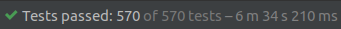
\includegraphics[width = 0.5\textwidth]{tests.png}
	\end{figure}

    Długi czas wykonywania testów wynika z przetwarzania dwóch, dużych plików. Jeden z nich ma rozmiar 8,4MB, a drugi 1,5MB. Obydwa zawierają dane wejściowe w~formacie \emph{DIMACS CNF}. 
	
	\section{Wyzwania implementowania w języku programowania \emph{Java}}\label{sec:AlgorytmPRozszerzenieTworzenieWstawienieDodawanieUwagi}
		
		Należy zwrócić szczególną uwagę na fakt, iż Knuth w swoim tłumaczeniu zakłada iteracje po indeksach zaczynających się od 1, podczas gdy \emph{Java} naturalnie przyjmuje indeksowanie od 0. W związku z tym należy dostosować algorytm tak, by brał to pod uwagę. W efekcie nasza implementacja drzewa \emph{Patricia} przyjmuje postać przedstawioną na rysunku~\ref{fig:PatriciaTreeJavaImplementation}.
		
		\begin{figure}[htb]
			\caption{Schemat drzewa \emph{Patricia} stworzonego przez implementacje w języku \emph{Java} w zgodności z algorytmem opisanym przez Knuth'a w ,,Sztuka programowania tom 3''~\cite{KnuthsTheArtOfComputerProgramming3}. Obrazuje przesunięcie pozycji klucza w pliku spowodowaną różnicą początkowego indeksu. Różnice można zauważyć porównując tę figurę względem figury~\ref{fig:PatriciaTree}.}\label{fig:PatriciaTreeJavaImplementation}
			\centering
			\begin{tikzpicture}[
			>={Stealth[inset=0pt,length=4pt, angle'=45,round]},
			nodeBox/.style = { rectangle, top color = white, bottom color = white, draw, black, text = black, minimum width = 1.25 cm, minimum height = 1.25 cm, font = \scriptsize, inner sep=0.05cm, outer sep=0.05cm },
			word/.style = { font = \scriptsize, inner sep=0.5pt, outer sep=0.5pt, text = black },
			greekSymbol/.style = { ellipse, minimum width = 0.5 cm, minimum height = 0.5 cm, fill, color = black, font = \small, inner sep=0pt, outer sep = 0pt, text = white },
			position/.style = { ellipse, minimum width = 0.5 cm, minimum height = 0.5 cm, top color = white, bottom color = white, draw, black, font = \scriptsize, inner sep=0pt, outer sep = 0pt, text = black}
			]
			
			\def\oneUnit{1.25cm}
			
			\node[nodeBox] (THISskip) at (-2*\oneUnit,1*\oneUnit) {$0$};
			\node[greekSymbol] (THISsymbol) at (-2.3*\oneUnit, 1.3*\oneUnit) {$0$};
			\node[position] (THISposition) at (-1.7*\oneUnit, 1.3*\oneUnit) {0};
			\node[word] (THIS) at (-2*\oneUnit, 0.65*\oneUnit) {(\texttt{THIS})};
			
			
			
			\node[nodeBox] (ISskip) at (-4*\oneUnit,-1*\oneUnit) {$0$};
			\node[greekSymbol] (ISsymbol) at (-4.3*\oneUnit, -0.7*\oneUnit) {$1$};
			\node[position] (ISposition) at (-3.7*\oneUnit,-0.7*\oneUnit) {5};
			\node[word] (IS) at (-4*\oneUnit, -1.35*\oneUnit) {(\texttt{IS})};
			
			
			
			\node[nodeBox] (BUILTskip) at (-7.5*\oneUnit,-3*\oneUnit) {$1$};
			\node[greekSymbol] (BUILTsymbol) at (-7.8*\oneUnit, -2.7*\oneUnit) {$6$};
			\node[position] (BUILTposition) at (-7.2*\oneUnit,-2.7*\oneUnit) {28};
			\node[word] (BUILT) at (-7.5*\oneUnit, -3.35*\oneUnit) {(\texttt{BUILT})};
			
			\node[nodeBox] (THEskip) at (-0.5*\oneUnit,-3*\oneUnit) {$11$};
			\node[greekSymbol] (THEsymbol) at (-0.8*\oneUnit, -2.7*\oneUnit) {$2$};
			\node[position] (THEposition) at (-0.2*\oneUnit,-2.7*\oneUnit) {8};
			\node[word] (THE) at (-0.5*\oneUnit, -3.35*\oneUnit) {(\texttt{THE})};
			
			
			
			\node[nodeBox] (JACKskip) at (-6*\oneUnit,-5*\oneUnit) {$2$};
			\node[greekSymbol] (JACKsymbol) at (-6.3*\oneUnit, -4.7*\oneUnit) {$5$};
			\node[position] (JACKposition) at (-5.7*\oneUnit,-4.7*\oneUnit) {23};
			\node[word] (JACK) at (-6*\oneUnit, -5.35*\oneUnit) {(\texttt{JACK})};
			
			\node[nodeBox] (THATskip) at (-2*\oneUnit,-5*\oneUnit) {$1$};
			\node[greekSymbol] (THATsymbol) at (-2.3*\oneUnit, -4.7*\oneUnit) {$4$};
			\node[position] (THATposition) at (-1.7*\oneUnit,-4.7*\oneUnit) {18};
			\node[word] (THAT) at (-2*\oneUnit, -5.35*\oneUnit) {(\texttt{THAT})};
			
			
			
			\node[nodeBox] (HOUSEskip) at (-7.5*\oneUnit,-7*\oneUnit) {$1$};
			\node[greekSymbol] (HOUSEsymbol) at (-7.8*\oneUnit, -6.7*\oneUnit) {$3$};
			\node[position] (HOUSEposition) at (-7.2*\oneUnit,-6.7*\oneUnit) {12};
			\node[word] (HOUSE) at (-7.5*\oneUnit, -7.35*\oneUnit) {(\texttt{HOUSE})};
			
			\draw [->] (THISskip) -- node[yshift = -0.25*\oneUnit, xshift = -0.5*\oneUnit] {\tiny $0$} ++ (-2*\oneUnit, 0*\oneUnit) -- (ISskip);
			
			\draw [->] (ISskip) -- node[yshift = -0.25*\oneUnit, xshift = -1.25*\oneUnit] {\tiny $0$} ++ (-3.5*\oneUnit, 0*\oneUnit) -- (BUILTskip);
			\draw [->] (ISskip) -- node[yshift = -0.25*\oneUnit, xshift = 1.25*\oneUnit] {\tiny $0$} ++ (3.5*\oneUnit, 0*\oneUnit) -- (THEskip);
			
			\draw [->, dashed] (BUILTskip) -- node[yshift = -1.25*\oneUnit, xshift = -0.25*\oneUnit] {\tiny $1$} ++(-1.5*\oneUnit, 0*\oneUnit) -- ++(0*\oneUnit, -1.5*\oneUnit) -- ++(1.5*\oneUnit, 0*\oneUnit) -- (BUILTskip);
			\draw [->] (BUILTskip) -- node[yshift = -0.25*\oneUnit, xshift = 0.25*\oneUnit] {\tiny $0$} ++(1.5*\oneUnit, 0*\oneUnit) -- (JACKskip);
			
			\draw [->] (THEskip) -- node[yshift = -0.25*\oneUnit, xshift = -0.25*\oneUnit] {\tiny $0$} ++(-1.5*\oneUnit, 0*\oneUnit) -- (THATskip);
			\draw [->, dashed] (THEskip) -- node[yshift = 2.0*\oneUnit, xshift = 0.25*\oneUnit] {\tiny $1$} ++ (1.5*\oneUnit, 0*\oneUnit) -- ++ (0*\oneUnit, 4*\oneUnit) -- (THISskip);
			
			
			\draw [->, dashed] (THATskip) -- node[yshift = -1.25*\oneUnit, xshift = -0.25*\oneUnit] {\tiny $1$} ++(-1.5*\oneUnit, 0*\oneUnit) -- ++(0*\oneUnit, -1.5*\oneUnit) -- ++(1.5*\oneUnit, 0*\oneUnit) -- (THATskip);
			\draw [->, dashed] (THATskip) -- node[yshift = 0.25*\oneUnit, xshift = 0.25*\oneUnit] {\tiny $1$} ++ (1.5*\oneUnit, 0*\oneUnit) -- (THEskip);
			
			\draw [->] (JACKskip) -- node[yshift = -0.25*\oneUnit, xshift = -0.25*\oneUnit] {\tiny $0$} ++(-1.5*\oneUnit, 0*\oneUnit) -- (HOUSEskip);
			\draw [->, dashed] (JACKskip) -- node[yshift = -1.25*\oneUnit, xshift = 0.25 cm] {\tiny $1$} ++(1.5*\oneUnit, 0*\oneUnit) -- ++(0*\oneUnit, -1.5*\oneUnit) -- ++(-1.5*\oneUnit, 0*\oneUnit) -- (JACKskip);
			
			\draw [->, dashed] (HOUSEskip) -- node[yshift = -1.25*\oneUnit, xshift = -0.25*\oneUnit] {\tiny $1$} ++(-1.5*\oneUnit, 0*\oneUnit) -- ++(0*\oneUnit, -1.5*\oneUnit) -- ++(1.5*\oneUnit, 0*\oneUnit) -- (HOUSEskip);
			\draw [->, dashed] (HOUSEskip) -- node[yshift = -0.25*\oneUnit, xshift = 1.75*\oneUnit] {\tiny $1$} ++(3.5*\oneUnit, 0*\oneUnit) -- (ISskip);
			\end{tikzpicture}
			
			\begin{tikzpicture}[
			>={Stealth[inset=0pt,length=4pt, angle'=45,round]},
			nodeBox/.style = { rectangle, top color = white, bottom color = white, draw, black, text = black, minimum width = 1.25 cm, minimum height = 1.25 cm, font = \scriptsize, inner sep=0.05cm, outer sep=0.05cm },
			word/.style = { font = \scriptsize, inner sep=0.5pt, outer sep=0.5pt, text = black },
			greekSymbol/.style = { ellipse, minimum width = 0.5 cm, minimum height = 0.5 cm, fill, color = black, font = \small, inner sep=0pt, outer sep = 0pt, text = white },
			position/.style = { ellipse, minimum width = 0.5 cm, minimum height = 0.5 cm, top color = white, bottom color = white, draw, black, font = \scriptsize, inner sep=0pt, outer sep = 0pt, text = black}
			]
			
			\def\oneUnit{1.25cm}
			
			\node[nodeBox] (LEGENDskip) at (0*\oneUnit,0*\oneUnit) {-1};
			\node[greekSymbol] (LEGENDsymbol) at (-0.3*\oneUnit, 0.3*\oneUnit) {$L$};
			\node[position] (LEGENDposition) at (0.3*\oneUnit, 0.3*\oneUnit) {0};
			\node[word] (LEGEND) at (0*\oneUnit, -0.35*\oneUnit) {(\texttt{LEGEND})};
			
			\node[word] (descriptionGreekSymbol) at (-2.5*\oneUnit, 0.275*\oneUnit) {Symbol identyfikujący węzeł};
			\node[word] (descriptionPosition) at (3.5*\oneUnit, 0.275*\oneUnit) {Numer pozycji w pliku, na którą wskazuje węzeł};
			\node[word] (descriptionSkip) at (-2.5*\oneUnit, -0.025*\oneUnit) {Ilość pozycji do przeskoczenia};
			\node[word] (descriptionArrows) at (5.5*\oneUnit, 0*\oneUnit) {\emph{LLINK} lub \emph{RLINK} zależnie z której strony wychodzi gałąź};
			\node[word] (descriptionWord) at (3.5*\oneUnit, -0.375*\oneUnit) {Słowo w pliku, na którego początek wskazuje numer pozycji};
			
			\draw [->] (-1.15*\oneUnit, 0.3*\oneUnit) -- (LEGENDsymbol);
			\draw [->] (1.25*\oneUnit, 0.3*\oneUnit) -- (LEGENDposition);
			\draw [->] (-1.1*\oneUnit, 0*\oneUnit) -- (-0.2*\oneUnit,0*\oneUnit);
			\draw [->] (0.75*\oneUnit, -0.35*\oneUnit) -- (LEGEND);
			\draw [->] (LEGENDskip) -- node[above = -0.1925*\oneUnit] {\contour{white}{\scriptsize \emph{LTAG} lub \emph{RTAG}}} (descriptionArrows);
			\end{tikzpicture}
		\end{figure}
		
		Kolejną przeszkodą stojącą na drodze implementacji dokładnie takiego samego przykładu jak ten podany w książce ,,Sztuka programowania tom 3''~\cite{KnuthsTheArtOfComputerProgramming3}  jest używana przez Knuth'a reprezentacja binarna, której bajty mają długość 5 bitów. \newpage Na dodatek, Knuth dla swojej maszyny \emph{MIX} zakłada kodowanie znaków, które znacząco różni się od tego występującego w języku \emph{Java}. Kodowanie, którego używa pokazane jest w tablicy~\ref{tab:MixMachineEncodingTable}. Oprócz różnicy w tym, jaki kod znaku (liczba całkowita) przypada znakowi (na przykład literze) w maszynie \emph{MIX} pojawiają się znaki niewystępujące w tablicy \emph{ASCII}, takie jak $\theta$, $\Phi$ czy $\Pi$. Mówiąc w tym miejscu o kodzie znaku, mamy na myśli wartość całkowitą otrzymywaną po rzutowaniu zmiennej typu \emph{char} (znaku) na \emph{int}. Wiąże się to z brakiem możliwości ograniczenia z góry zawartości plików do znaków kodowanych na pojedynczym bajcie przy kodowaniu \emph{UTF-8}.
		
		\begin{table}[htb]
			\centering
			\begin{threeparttable}
				\caption{Tablica kodowania znaków maszyny \emph{MIX} zasięgnięta z \url{https://esolangs.org/wiki/MIX_(Knuth)}~\cite{wikiMix}. Znak posiadający kod 0 to spacja, z tego powodu jest niewidoczny.}\label{tab:MixMachineEncodingTable}
				{ \small
					\begin{tabularx}{0.705\textwidth}{C{5}|C{1}|C{1}|C{1}|C{1}|C{1}|C{1}|C{1}|C{1}|C{1}|C{1}|}
						\textbf{Kod znaku} & 0 & 1 & 2 & 3 & 4 & 5 & 6 & 7 & 8 & 9 \\
						\textbf{Znak}      &   & A & B & C & D & E & F & G & H & I \\
						\hline \hline
						\textbf{Kod znaku} & 10 & 11 & 12 & 13 & 14 & 15 & 16 & 17 & 18 & 19 \\
						\textbf{Znak}      &$\theta$& J & K & L & M & N & O & P & Q & R \\
						\hline \hline
						\textbf{Kod znaku} & 20 & 21 & 22 & 23 & 24 & 25 & 26 & 27 & 28 & 29 \\
						\textbf{Znak}      &$\Phi$&$\Pi$& S & T & U & V & W & X & Y & Z \\
						\hline \hline
						\textbf{Kod znaku} & 30 & 31 & 32 & 33 & 34 & 35 & 36 & 37 & 38 & 39 \\
						\textbf{Znak}      &  0 & 1 & 2 & 3 & 4 & 5 & 6 & 7 & 8 & 9 \\
						\hline \hline
						\textbf{Kod znaku} & 40 & 41 & 42 & 43 & 44 & 45 & 46 & 47 & 48 & 49 \\
						\textbf{Znak}      & . & , & ( & ) & + & - & * & / & = & \$ \\
						\hline \hline
						\textbf{Kod znaku} & 50 & 51 & 52 & 53 & 54 & 55 & & & & \\
						\textbf{Znak}      & < & > & @ & ; & : & ' & & & & \\
						\hline \hline
					\end{tabularx} 
				}
			\end{threeparttable}
		\end{table}
		
		Ma to znaczenie, gdyż w swojej implementacji chcieliśmy wykorzystać klasę \emph{RandomAccessFile}, która odczytuje plik niekoniecznie od jego początku, krok po kroku, przechodząc do fragmentu w którym chcemy wykonać daną operację. Ma ona możliwość odczytu pliku w podawanym poprzez parametr miejscu -- danym indeksem bajtu zaczynającym się od 0. 
		
		Występowanie znaków z poza tablicy \emph{ASCII} w tablicy znaków maszyny \emph{MIX} oznacza, że nie możemy przyjąć założenia ułatwiającego -- sprawiającego, że indeks bajtu zawsze jest równy indeksowi znaku. Oprócz śledzenia tej różnicy musimy obsłużyć odczytywanie odpowiedniej ilości bajtów (1, 2, 3 lub 4 bajty) na podstawie pierwszego bajtu znaku oraz dekodowanie ich tworząc obiekt klasy \emph{String}, która z kolei jest przechowywania w pamięci wirtualnej maszyny języka \emph{Java} zgodnie z tablicą kodowania znaków \emph{UTF-16}. Dodatkowo Knuth wykorzystuje w swoim oryginalnym przykładzie znak zapytania (?), który nie pojawia się w tablicy znaków maszyny \emph{MIX}. Na szczęście pełni on funkcję unikatowego znaku końca klucza, co oznacza, że można zastąpić go wolnym znakiem obecnym w tablicy znaków maszyny \emph{MIX}. Nadpisując metody \emph{toString()} odpowiednich klas możemy uzyskać reprezentację tekstową drzewa, która może przyjmować postać przedstawioną na następnej stronie, w kodzie źródłowym~\ref{programReprezentacjaKlasyImplementujacejPatricia}.
		
		\begin{program}
			\caption{Przykładowa tekstowa reprezentacja obiektu klasy implementującej drzewo \emph{Patricia}. Reprezentuje ona to samo drzewo co figura~\ref{fig:PatriciaTreeJavaImplementation} tylko w postaci tekstowej. Wynik metody nadpisanej \emph{toString()}.}\label{programReprezentacjaKlasyImplementujacejPatricia}
			\begin{lstlisting}[basicstyle=\scriptsize,]
PatriciaTree{
	// [...] 
	header = PatriciaNode{
	id = 0,
	key = 0,
	skip = 0,
	isLeftAncestor = false,
	isRightAncestor = false,
	leftLink = PatriciaNode{
		id = 1,
		key = 7,
		skip = 1,
		isLeftAncestor = false,
		isRightAncestor = false,
		leftLink = PatriciaNode{
			id = 6,
			key = 42,
			skip = 1,
			isLeftAncestor = true,
			isRightAncestor = false,
			leftLink.id = 6,
			rightLink = PatriciaNode{
				id = 5,
				key = 35,
				skip = 2,
				isLeftAncestor = false,
				isRightAncestor = true,
				leftLink = PatriciaNode{
					id = 3,
					key = 20,
					skip = 1,
					isLeftAncestor = true,
					isRightAncestor = true,
					leftLink.id = 3,
					rightLink.id = 1
				},
				rightLink.id = 5
			}
		},
		rightLink = PatriciaNode{
			id = 2,
			key = 14,
			skip = 13,
			isLeftAncestor = false,
			isRightAncestor = true,
			leftLink = PatriciaNode{
				id = 4,
				key = 28,
				skip = 1,
				isLeftAncestor = true,
				isRightAncestor = true,
				leftLink.id = 4,
				rightLink.id = 2
			},
			rightLink.id = 0
		}
	},
	rightLink = null
}
	// [...]
}
			\end{lstlisting}
		\end{program}
	
	    \section{Implementacja kodowania znaków oraz reprezentacji bitowej maszyny \emph{MIX}}\label{sec:czescPraktycznaImplementacjaMIX}
	    
	    Implementując pierwszą wersję klasy drzewa \emph{Patricia} chcieliśmy osiągnąć wyniki jak najbardziej zbliżone do podanych przez Knuth'a przykładów. 
	    
	    W tym celu stworzyliśmy klasę \emph{MixByte} symulującą reprezentację binarną maszyny \emph{MIX}, a dokładniej jej pojedynczego bajtu. Klasa \emph{MixByte} w swoim konstruktorze, jako parametr, przyjmuje pożądaną długość bajtu. Utworzyliśmy również klasę \emph{MixEncoding} symulującą kodowanie znaków maszyny \emph{MIX} według tablicy~\ref{tab:MixMachineEncodingTable}. Zmodyfikowaliśmy ją jednak tak, aby zagwarantować, że podawane przez parametry konstruktora znaki końca pliku i końca klucza zawsze będą zawarte w tablicy znaków symulowanej maszyny. Znak końca pliku za każdym razem jest umieszczany w miejsce znaku `1` (kod znaku 31), a znak końca klucza zawsze w miejsce znaku `0` (kod znaku 30) zgodnie z tabelą przedstawioną w~tablicy~\ref{tab:ModifiedMixMachineEncodingTable}. Oznacza to, że gwarancja istnienia tych znaków w~tablicy symulowanej maszyny dotyczy tylko maszyny, której bajt ma długość co najmniej 5 bitów. Znaczenie tych znaków zostaje wytłumaczone w następnych rozdziałach~\ref{sec:czescPraktycznaImplementacjaDrzewaPatriciaKnuth} oraz~\ref{sec:czescPraktycznaImplementacjaDrzewaPatriciaAutorska}.
	    
	    \begin{table}[htb]
			\centering
			\begin{threeparttable}
				\caption{Zmodyfikowana tablica kodowania znaków maszyny \emph{MIX} tak, aby gwarantować istnienie sparametryzowanych znaków końca pliku i końca klucza, w symulowanej maszynie, której długość bajtu wynosi co najmniej 5 bitów. Znak oznaczony przez \emph{EOF} to znak końca pliku (ang. \emph{End Of File character}), a znak oznaczony przez \emph{EOK} to znak końca klucza (ang. \emph{End Of Key character}). Tablica zasięgnięta z \url{https://esolangs.org/wiki/MIX_(Knuth)}~\cite{wikiMix}. Znak posiadający kod 0 to spacja, z tego powodu jest niewidoczny.}\label{tab:ModifiedMixMachineEncodingTable}
				{ \small
					\begin{tabularx}{0.96\textwidth}{C{5}|C{2}|C{2}|C{2}|C{2}|C{2}|C{2}|C{2}|C{2}|C{2}|C{2}|}
						\textbf{Kod znaku} & 0 & 1 & 2 & 3 & 4 & 5 & 6 & 7 & 8 & 9 \\
						\textbf{Znak}      &   & A & B & C & D & E & F & G & H & I \\
						\hline \hline
						\textbf{Kod znaku} & 10 & 11 & 12 & 13 & 14 & 15 & 16 & 17 & 18 & 19 \\
						\textbf{Znak}      &$\theta$& J & K & L & M & N & O & P & Q & R \\
						\hline \hline
						\textbf{Kod znaku} & 20 & 21 & 22 & 23 & 24 & 25 & 26 & 27 & 28 & 29 \\
						\textbf{Znak}      &$\Phi$&$\Pi$& S & T & U & V & W & X & Y & Z \\
						\hline \hline
						\textbf{Kod znaku} & 30 & 31 & 32 & 33 & 34 & 35 & 36 & 37 & 38 & 39 \\
						\textbf{Znak}      & EOK & EOF & 2 & 3 & 4 & 5 & 6 & 7 & 8 & 9 \\
						\hline \hline
						\textbf{Kod znaku} & 40 & 41 & 42 & 43 & 44 & 45 & 46 & 47 & 48 & 49 \\
						\textbf{Znak}      & . & , & ( & ) & + & - & * & / & = & \$ \\
						\hline \hline
						\textbf{Kod znaku} & 50 & 51 & 52 & 53 & 54 & 55 & & & & \\
						\textbf{Znak}      & < & > & @ & ; & : & ' & & & & \\
						\hline \hline
					\end{tabularx} 
				}
			\end{threeparttable}
		\end{table}
	    
	    Scalając te dwie klasy w postać klasy \emph{MixMachine} osiągnęliśmy rezultat prawie identyczny do przykładu przedstawionego przez Knuth'a w jego książce. Jedyną różnicą jest przesunięcie o 1 wartości pola \emph{KEY}. Wynika ono z innego indeksowania pozycji znaku w pliku, które w naszej implementacji wynosi 0, a nie 1, jak w oryginale. Różnicę można zauważyć porównując rysunek~\ref{fig:PatriciaTree} (przykład Knuth'a) oraz rysunek~\ref{fig:PatriciaTreeJavaImplementation} (nasza implementacja).
	    
		\section{Implementacja drzewa \emph{Patricia} -- w zgodności z wymaganiami Knuth'a}\label{sec:czescPraktycznaImplementacjaDrzewaPatriciaKnuth}
		
		Algorytmy wyszukiwania listy węzłów akceptujących argument wyszukiwania jako prefiks (opisany w niniejszej pracy w rozdziale~\ref{sec:AlgorytmPRozszerzenieWyszukiwanie}) oraz wstawiania nowych węzłów do drzewa (opisany w niniejszej pracy w rozdziale~\ref{sec:AlgorytmPRozszerzenieTworzenieWstawienieDodawanie}) przedstawione w książce Knuth'a~ \cite{KnuthsTheArtOfComputerProgramming3} były dla nas z początku niejasnymi fragmentami. Dzięki zabiegom opisanym wcześniej mogliśmy pozwolić sobie na przetestowanie naszych domysłów. Takie podejście pozwoliło nam zdecydowanie wcześniej przystąpić do implementacji, rozwiać wątpliwości, odpowiedzieć na pojawiające się w trakcie pytania oraz opisać w sposób bardziej szczegółowy wszystko, czego dowiedzieliśmy się w tym procesie.
		
		Algorytm P \ref{sec:AlgorytmP} (sprawdzający czy słowo dane jako parametr jest prefiksem, któregoś z kluczy w drzewie) jest w zaimplementowany w postaci metody \emph{isContainingPrefix(String searchWord)} klasy \emph{PatriciaTree}. 
		
		\emph{findNodesMatchingPrefix(String searchWord)} tej samej klasy jest metodą implementującą algorytm rozszerzający algorytm P~\ref{sec:AlgorytmPRozszerzenieWyszukiwanie} (wyszukujący listę węzłów zawierających klucze akceptujące słowo dane parametrem jako prefiks). 
		
		Metoda \emph{insertNextKeyIntoTree()} również należąca do klasy \emph{PatriciaTree} jest metodą wstawiającą następny węzeł zawarty do struktury drzewa. Działa ona zgodnie z algorytmem opisanym w sekcji~\ref{sec:AlgorytmPRozszerzenieTworzenieWstawienieDodawanie}. Oprócz zasady działania opisanej w tej sekcji kluczowymi metodami wykorzystywanymi w naszej implementacji są metody \emph{findNextWordStartIndex(int latestInsertedNodeKeyPosition)} oraz \emph{getWordStringFromFileStartingAtPosition(int newKeyStartIndex)} klasy \emph{FileOps} (a dokładniej -- jej pola klasy rozszerzającej klasę \emph{FileOpsStrategy}).
		
		Metoda \emph{findNextWordStartIndex(int latestInsertedNodeKeyPosition)} zwraca pozycję (indeks bajtu w pliku) początku następnego do wstawienia klucza -- na podstawie argumentu będącego pozycją początku ostatnio wstawionego klucza.
		
		Metoda \emph{getWordStringFromFileStartingAtPosition(int newKeyStartIndex)} zwraca klucz (w postaci obiektu klasy \emph{String}) -- na podstawie pozycji w której on się zaczyna w~pliku.
		
		\emph{insertAllKeysIntoTree()} jest metodą, która jest naturalnym rozszerzeniem operacji wstawienia pojedynczego klucza do drzewa \emph{Patricia}. Jej działanie jest zaskakująco proste. Wykorzystuje metodę \emph{insertNextKeyIntoTree()} w pętli bez warunku końca. Zatrzymanie pętli odbywa się poprzez wyłapanie (ang. \emph{catch}) wyjątku \emph{NextWordStartIndexNotFoundException} wyrzucanego (ang. \emph{throw}) przez metodę odpowiedzialną za znajdowanie pozycji startowej następnego klucza do dodania do drzewa.\newpage
		
        Tak jak wspomnieliśmy w poprzednim podrozdziale -- oprócz tego udało się nam osiągnąć prawie identyczne wyniki jak te podane przy opisach Knuth'a. Dzięki temu mogliśmy przetestować możliwości implementacji naszych klas, ich parametryzowania oraz ograniczenia zaimplementowanych algorytmów. Natchnęło nas to do podjęcia próby modyfikacji tych algorytmów tak, aby klucze w drzewie \emph{Patricia} przypominały bardziej klucze opisywane w innych algorytmach (dotyczących drzew \emph{Trie}). Chcieliśmy, aby klucze mogły być pojedynczymi słowami, a nie były ograniczone do bycia fragmentem jednego zdania.
		
		\section{Implementacja drzewa \emph{Patricia} -- autorski algorytm}\label{sec:czescPraktycznaImplementacjaDrzewaPatriciaAutorska}
		
		Pod koniec procesu opisanego w poprzednim podrozdziale~\ref{sec:czescPraktycznaImplementacjaDrzewaPatriciaKnuth} zdaliśmy sobie sprawę z faktu iż, algorytmy dotyczące drzewa \emph{Patricia} opisane przez Knuth'a nie mają możliwości wykorzystania w praktyce różnicy między prefiksem, a kluczem dla opisanych przez niego operacji. Jest to konsekwencją unikalnego sposobu definiowania klucza w porównaniu do pozostałych algorytmów opisanych w tym rozdziale. 
		
		Knuth w swojej książce w kontekście drzewa \emph{Patricia} definiuje klucz jako fragment pliku zaczynający się w pozycji startowej $x$ klucza, aż do końca pliku, jednocześnie zakładając, że plik -- będący zbiorem kluczy -- jest bardzo długi. Prawdą jest, że dla bardzo specyficznego przypadku, kiedy każdy z kluczy jest prefiksem drugiego (nie licząc unikalnego znaku końca pliku) algorytm Knuth'a jest optymalny. Chcieliśmy jednak, aby nasza implementacja była przystosowana do szerszego zakresu problemów. W związku z tym w naszej modyfikacji algorytmu skupiliśmy się na tym, aby klucze mogły być pojedynczymi słowami. W efekcie udało się nam zmodyfikować algorytm Knuth'a tak, aby kluczami mogły być jednocześnie słowa i frazy. Różnica w sposobie definiowania klucza przedstawiona jest na rysunku~\ref{fig:strategySingleWordVsSPTEOF} znajdującym się na następnej stronie.
		
		Motywacją do podjęcia się tej modyfikacji było to, że dla przypadku, który nie jest tym szczególnym, lecz tym bardziej ogólnym, w którym chcielibyśmy, aby dało się w~drzewie przetrzymywać zbiór kluczy, w którym niekoniecznie każdy jest prefiksem innego (nie licząc znaku końca pliku) -- algorytm Knuth'a jest naszym zdaniem nieoptymalny.
		
		Nie widzimy powodu, dla którego sprawdzanie czy dany klucz należy do zbioru kluczy akceptowanych przez drzewo \emph{Patricia}, czy wyszukiwanie węzła zawierającego klucz jest praktyczne w przypadku, gdy klucz jest długim ciągiem znaków (należących nie tylko do klucza, który nas na prawdę interesuje). 
		
		Dodatkową wadą szkicu implementacji przedstawionej przez Knuth'a dla sytuacji kiedy klucze są oddzielnymi ciągami znaków i klucz, o który chcemy zapytać drzewo \emph{Patricia} nie jest ostatnim w pliku jest fakt, że musimy znać nie tylko wszystkie klucze występujące po tym kluczu w pliku, ale również ich kolejność występowania.
		
		Z tego powodu postanowiliśmy stworzyć oddzielny wariant drzewa \emph{Patricia}, który definiowałby klucz jako fragment pliku, który zaczynałby się w pozycji startowej $x$, ale kończył po napotkaniu znaku końca klucza, który nazwaliśmy \emph{End Of Key character}. Dzięki temu pojedyncze klucze byłyby zdecydowanie krótsze i mogłyby być wykorzystywane w praktyce jako argumenty operacji przeszukiwania drzewa.
		
		Omawianą wariację drzewa \emph{Patricia} postanowiliśmy zaimplementować w postaci wzorca projektowego strategia (ang. \emph{strategy}). Wybór strategii odbywa się poprzez przekazanie jako parametru obiektu klasy \emph{WordStategy} typu \emph{enum} do konstruktora klasy \emph{FileOps}. Obiekt klasy \emph{enum} \emph{WordStrategy} przyjmuje 2 wartości \emph{WordStrategy.SINGLE} oraz \emph{WordStrategy.START\textunderscore POSITION\textunderscore TO\textunderscore EOF}. Dzięki temu klasa \emph{FileOps} wie, której klasy konstruktor wywołać - odpowiednio: \emph{WordSingleStrategy} lub \emph{WordStartPositionToEOFStrategy}.
		
		\begin{figure}
			\caption{Rysunek przestawia różnicę w sposobie definiowania klucza w implementacjach definiujących klucz. Obie klasy dziedziczą po abstrakcyjnej klasie \emph{FileOpsStrategy}. Wybór wykorzystywanej implementacji odbywa się poprzez przekazanie parametru klasy \emph{enum} \emph{WordStrategy} do konstruktora klasy \emph{FileOps}. Jest to przykład wykorzystania wzorca projektowego strategia (ang. \emph{strategy}). Oznaczenia i linie znajdujące się nad zdaniem dotyczą założeń Knuth'a a te, znajdujące się na samym dole -- naszego założenia.}\label{fig:strategySingleWordVsSPTEOF}
			\centering
			\begin{tikzpicture}[
			>={Stealth[inset=0pt,length=4pt, angle'=45,round]},
			word/.style = { font = \normalsize, inner sep=0.1pt, outer sep=0.1pt, text = black },
			fake/.style = { inner sep=0pt, outer sep=0pt },
			]
			
			\def\oneUnit{1.25cm}
			
			\node[word] (zawartoscPliku) at (0*\oneUnit, 0*\oneUnit) {THIS IS THE HOUSE THAT JACK BUILT;};
			
			\node[word] (wordStartPositionToEOFStrategy) at (0*\oneUnit, 2*\oneUnit) {Pole klasy: \emph{WordStartPositionToEOFStrategy extends FileOpsStrategy}};
			\node[word] (wordSingleStrategy) at (0*\oneUnit, -2.5*\oneUnit) {Pole klasy: \emph{WordSingleStrategy extends FileOpsStrategy}};
			
			
			\node[word] (fileOpsSPTEOF) at (0*\oneUnit, 2.5*\oneUnit) {Obiekt klasy: \emph{new FileOps(..., WordStrategy.START\textunderscore POSITION\textunderscore TO\textunderscore EOF, ...);}};
			\node[word] (fileOpsSingle) at (0*\oneUnit, -2*\oneUnit) {Obiekt klasy: \emph{new FileOps(..., WordStrategy.SINGLE, ...);}};
			
			\node[word] (implementacjaKnuth) at (0*\oneUnit, 3*\oneUnit) {Implementacja klucza zgodnie z wymaganiami algorytmów Knuth'a};
			\node[word] (implementacjaAutorska) at (0*\oneUnit, -1.5*\oneUnit) {Implementacja autorska klucza postaci pojedynczego słowa};
			
			\node[fake] (koniecZawartosciPliku) at (3.1*\oneUnit, 0*\oneUnit) {};
			\node[fake] (poczatekZawartosciPliku) at (-3.1*\oneUnit, 0*\oneUnit) {};
			
			\node[fake] (nadPoczatkiemZawartosciPliku) at (-3.1*\oneUnit, 1.4*\oneUnit) {};
			\node[fake] (podPoczatkiemZawartosciPliku) at (-3.1*\oneUnit, -0.5*\oneUnit) {};
			
			\node[fake] (nadKoncemZawartosciPliku1) at (3.1*\oneUnit, 1.4*\oneUnit) {};
			\node[fake] (nadKoncemZawartosciPliku2) at (3.1*\oneUnit, 1.25*\oneUnit) {};
			\node[fake] (nadKoncemZawartosciPliku3) at (3.1*\oneUnit, 1.1*\oneUnit) {};
			\node[fake] (nadKoncemZawartosciPliku4) at (3.1*\oneUnit, 0.95*\oneUnit) {};
			\node[fake] (nadKoncemZawartosciPliku5) at (3.1*\oneUnit, 0.8*\oneUnit) {};
			\node[fake] (nadKoncemZawartosciPliku6) at (3.1*\oneUnit, 0.65*\oneUnit) {};
			\node[fake] (nadKoncemZawartosciPliku7) at (3.1*\oneUnit, 0.5*\oneUnit) {};
			
			\node[fake] (podKoncemZawartosciPliku1) at (3.1*\oneUnit, -0.5*\oneUnit) {};
			
			\node[fake] (koniecThis) at (-2.25*\oneUnit, 0*\oneUnit) {};
			
			\node[fake] (nadKoniecThis1) at (-2.25*\oneUnit, 1.25*\oneUnit) {};
			\node[fake] (podKoniecThis1) at (-2.25*\oneUnit, -0.5*\oneUnit) {};
			
			\node[fake] (podKoniecThis2) at (-2.25*\oneUnit, -0.65*\oneUnit) {};
			
			\node[fake] (koniecIs) at (-1.85*\oneUnit, 0*\oneUnit) {};
			
			\node[fake] (nadKoniecIs1) at (-1.85*\oneUnit, 1.1*\oneUnit) {};
			\node[fake] (podKoniecIs1) at (-1.85*\oneUnit, -0.5*\oneUnit) {};
			
			\node[fake] (podKoniecIs2) at (-1.85*\oneUnit, -0.65*\oneUnit) {};
			
			\node[fake] (koniecThe) at (-1.1*\oneUnit, 0*\oneUnit) {};
			
			\node[fake] (nadKoniecThe1) at (-1.1*\oneUnit, 0.95*\oneUnit) {};
			\node[fake] (podKoniecThe1) at (-1.1*\oneUnit, -0.5*\oneUnit) {};
			
			\node[fake] (podKoniecThe2) at (-1.1*\oneUnit, -0.65*\oneUnit) {};
			
			\node[fake] (koniecHouse) at (0.1*\oneUnit, 0*\oneUnit) {};
			
			\node[fake] (nadKoniecHouse1) at (0.1*\oneUnit, 0.8*\oneUnit) {};
			\node[fake] (podKoniecHouse1) at (0.1*\oneUnit, -0.5*\oneUnit) {};
			
			\node[fake] (podKoniecHouse2) at (0.1*\oneUnit, -0.65*\oneUnit) {};
			
			\node[fake] (koniecThat) at (1.05*\oneUnit, 0*\oneUnit) {};
			
			\node[fake] (nadKoniecThat1) at (1.05*\oneUnit, 0.65*\oneUnit) {};
			\node[fake] (podKoniecThat1) at (1.05*\oneUnit, -0.5*\oneUnit) {};
			
			\node[fake] (podKoniecThat2) at (1.05*\oneUnit, -0.65*\oneUnit) {};
			
			\node[fake] (koniecJack) at (1.95*\oneUnit, 0*\oneUnit) {};
			
			\node[fake] (nadKoniecJack1) at (1.95*\oneUnit, 0.5*\oneUnit) {};
			\node[fake] (podKoniecJack1) at (1.95*\oneUnit, -0.5*\oneUnit) {};
			
			\node[fake] (podKoniecJack2) at (1.95*\oneUnit, -0.65*\oneUnit) {};
			
			\path (poczatekZawartosciPliku) edge [] (nadPoczatkiemZawartosciPliku);
			\path (poczatekZawartosciPliku) edge [] (podPoczatkiemZawartosciPliku);
			
			\path (koniecThis) edge [] (nadKoniecThis1);
			\path (koniecThis) edge [] (podKoniecThis1);
			
			\path (koniecThis) edge [] (podKoniecThis2);
			
			\path (koniecIs) edge [] (nadKoniecIs1);
			\path (koniecIs) edge [] (podKoniecIs1);
			
			\path (koniecIs) edge [] (podKoniecIs2);
			
			\path (koniecThe) edge [] (nadKoniecThe1);
			\path (koniecThe) edge [] (podKoniecThe2);
			
			\path (koniecThe) edge [] (nadKoniecThe1);
			\path (koniecThe) edge [] (podKoniecThe2);
			
			\path (koniecHouse) edge [] (nadKoniecHouse1);
			\path (koniecHouse) edge [] (podKoniecHouse1);
			
			\path (koniecHouse) edge [] (podKoniecHouse2);
			
			\path (koniecThat) edge [] (nadKoniecThat1);
			\path (koniecThat) edge [] (podKoniecThat1);
			
			\path (koniecThat) edge [] (podKoniecThat2);
			
			\path (koniecJack) edge [] (nadKoniecJack1);
			\path (koniecJack) edge [] (podKoniecJack1);
			
			\path (koniecJack) edge [] (podKoniecJack2);
			
			\path (koniecZawartosciPliku) edge [] (nadKoncemZawartosciPliku1);
			\path (koniecZawartosciPliku) edge [] (nadKoncemZawartosciPliku2);
			\path (koniecZawartosciPliku) edge [] (nadKoncemZawartosciPliku3);
			\path (koniecZawartosciPliku) edge [] (nadKoncemZawartosciPliku4);
			\path (koniecZawartosciPliku) edge [] (nadKoncemZawartosciPliku5);
			\path (koniecZawartosciPliku) edge [] (nadKoncemZawartosciPliku6);
			\path (koniecZawartosciPliku) edge [] (nadKoncemZawartosciPliku7);
			
			\path (koniecZawartosciPliku) edge [] (podKoncemZawartosciPliku1);
			
			\path (nadPoczatkiemZawartosciPliku) edge [] node[above = -0.25 cm] {\tiny \contour{white}{$K_1$}} (nadKoncemZawartosciPliku1);
			\path (nadKoniecThis1) edge [] node[above = -0.25 cm] {\tiny \contour{white}{$K_2$}} (nadKoncemZawartosciPliku2);
			\path (nadKoniecIs1) edge [] node[above = -0.25 cm] {\tiny \contour{white}{$K_3$}} (nadKoncemZawartosciPliku3);
			\path (nadKoniecThe1) edge [] node[above = -0.25 cm] {\tiny \contour{white}{$K_4$}} (nadKoncemZawartosciPliku4);
			\path (nadKoniecHouse1) edge [] node[above = -0.25 cm] {\tiny \contour{white}{$K_5$}} (nadKoncemZawartosciPliku5);
			\path (nadKoniecThat1) edge [] node[above = -0.25 cm] {\tiny \contour{white}{$K_6$}} (nadKoncemZawartosciPliku6);
			\path (nadKoniecJack1) edge [] node[above = -0.25 cm] {\tiny \contour{white}{$K_7$}} (nadKoncemZawartosciPliku7);
			
			\path (podPoczatkiemZawartosciPliku) edge [] node[above = -0.25 cm] {\tiny \contour{white}{$K_1$}} (podKoniecThis1);
			\path (podKoniecThis2) edge [] node[above = -0.25 cm] {\tiny \contour{white}{$K_2$}} (podKoniecIs2);
			\path (podKoniecIs1) edge [] node[above = -0.25 cm] {\tiny \contour{white}{$K_3$}} (podKoniecThe1);
			\path (podKoniecThe2) edge [] node[above = -0.25 cm] {\tiny \contour{white}{$K_4$}} (podKoniecHouse2);
			\path (podKoniecHouse1) edge [] node[above = -0.25 cm] {\tiny \contour{white}{$K_5$}} (podKoniecThat1);
			\path (podKoniecThat2) edge [] node[above = -0.25 cm] {\tiny \contour{white}{$K_6$}} (podKoniecJack2);
			\path (podKoniecJack1) edge [] node[above = -0.25 cm] {\tiny \contour{white}{$K_7$}} (podKoncemZawartosciPliku1);
			
			\end{tikzpicture}
		\end{figure}
		
		Dodatkowo klasy wykorzystywane w implementacji wzorca projektowego strategia przyjmują jako parametry typu \emph{char} znak końca pliku (\emph{charEOF}) oraz znak końca klucza (\emph{charEOK}). Dzięki \emph{charEOF} wiedzą, jaki znak interpretować jako kończący listę kluczy. Dzięki \emph{charEOK} klasa \emph{WordSingleStrategy} wie, który znak oznacza koniec klucza. Znaki końca klucza i końca pliku są zaliczane do klucza i pojawiają się na jego końcu. Jeżeli kilka znaków końca klucza pojawia się po kluczu to wszystkie są uznawane za jego część (ostatni znak końca klucza kończy go). Jeżeli jakikolwiek znak istnieje po znaku końca pliku to nie jest on brany pod uwagę przy analizie kluczy. \newpage Innymi słowy -- jeżeli \emph{charEOF} pojawi się na pozycji $x$ to nie ma klucza na pozycji większej od $x$. Jeżeli istnieje ciąg znaków końca klucza po jakimś kluczu, a po tym ciągu pojawia się znak końca pliku to wszystkie znaki \emph{charEOK} i \emph{charEOF} są uznawane za część klucza.
		
		Oprócz metod opisanych w poprzedniej sekcji, konsekwencją implementacji nowej strategii była implementacja dwóch dodatkowych metod, które odpowiadały na pytania dotyczące kluczy zamiast prefiksów.
		
		Metoda \emph{isContainingKey(String searchWord)} klasy \emph{PatriciaTree} jest metodą analogiczną do wcześniej opisanej i zaimplementowanej funkcjonalności \emph{isContainingPrefix(String searchWord)}, a dodatkowo ją wykorzystuje. Zastosowaliśmy tutaj właściwość metody dotyczącej prefiksów. Zauważyliśmy, że wystarczającym warunkiem, aby prefiks był kluczem jest równość długości argumentu \emph{searchWord} oraz klucza zawartego w węźle akceptującym argument jako prefiks. Jeżeli jednak argument \emph{searchWord} nie jest prefiksem żadnego z kluczy to nie jest on też kluczem.
		
		Metoda \emph{findNodeMatchingKey(String searchWord)} klasy \emph{PatriciaTree} jest metodą analogiczną do wcześniej opisanej i zaimplementowanej funkcjonalności \emph{findNodesMatchingPrefix(String searchWord)}. Różnicą między tymi dwoma metodami jest fakt, że \emph{findNodesMatchingPrefix(String searchWord)} zwraca tablicę węzłów drzewa \emph{Patricia} (\emph{PatriciaNode[]}) -- akceptujących argument przeszukiwania jako prefiks klucza zawartego w nich -- podczas gdy \emph{findNodeMatchingKey(String searchWord)} zwraca jeden węzeł drzewa -- którego zawarty w nim klucz jest równy argumentowi wyszukiwania. Nowa metoda odpowiadającą na pytanie dotyczące charakterystyki kluczy drzewa, podobnie jak metoda dotycząca charakterystyki prefiksów, wykorzystuje wcześniej zaimplementowaną metodę \emph{isContaining}, lecz jest nią metoda \emph{isContainingKey} zamiast \emph{isContainingPrefix}.
		
		Rysunek \ref{fig:classDiagram} w załączniku do pracy przedstawia diagram klas paczki \emph{agh.jo.knuth} wyeksportowany ze środowiska programowani \emph{IntelliJ IDEA}.
				
		\section{Koniunkcyjna postać normalna w drzewie \emph{Patricia} -- wykorzystanie implementacji w rozwiązaniu problemu praktycznego}\label{sec:czescPraktycznaCNF}
		
		Praktycznym problemem postawionym przed implementacją autorską drzewa \emph{Patricia} stały się pliki \emph{DIMACS CNF} reprezentujące koniunkcyjną postać normalną. Pliki te, ich format oraz samo pojęcie koniunkcyjnej postaci normalnej zostały opisane w sekcji~\ref{sec:CNF}. Autorska implementacja drzewa \emph{Patricia} miała przetrzymywać zbiór klauzul umieszczony w pliku o rozszerzeniu \emph{*.cnf}. Przykład fragmentu takiego pliku wykorzystanego do testowania tej implementacji można zobaczyć w kodzie źródłowym~\ref{prog:CNFsourceFile}. \newpage
				
		\begin{program}
			\caption{Przykład fragmentu pliku w formacie \emph{DIMACS CNF} o nazwie ``Analiza1-gss-20-s100.cnf`` wykorzystanego w kodzie źródłowym~\ref{prog:CnfConverterAndPatriciaTreeConstrutorsParamatersRelationship}. Plik ma rozmiar równy 1.5 Mb.}\label{prog:CNFsourceFile}
    		\begin{lstlisting}[basicstyle=\scriptsize,]
c 100 20
// [...]
p cnf 31503 94748
7272 0
30549 0
7270 0
30550 0
30551 0
30552 0
7314 0
30553 0
7268 0
7267 0
// [...]
-31503 -442 -24184 0
31503 -442 24184 0
31503 442 -24184 0
// NL at the end of file
    		\end{lstlisting}
		\end{program}
		
		Implementacja ta miała pozwalać uzyskać odpowiedź na pytania pokroju -- czy klauzula $x$ znajduje się w zbiorze klauzul? Jednocześnie powinna ona jak najlepiej grupować klauzule o podobnych podzbiorach literałów. Doszliśmy do wniosku, że odpowiedź na pierwsze pytanie można uzyskać poprzez użycie metody \emph{isContainingKey}, czy \emph{findNodeMatchingKey} klasy \emph{PatriciaTree}. Do znalezienia klauzul o podzbiorze literałów podobnym do zbioru innej klauzuli najlepiej nadaje się metoda \emph{findNodesMatchingPrefix}. Nie jest to oczywiście idealne rozwiązanie ze względu na definicję prefiksu, gdyż różnica w~pierwszych literałach dyskwalifikuje dany węzeł jako ten zawierający klucz akceptujący argument przeszukiwania jako prefiks.
		
		Dzięki wysokiemu poziomu możliwości dostosowania klasy \emph{PatriciaTree} problem ten nie stawiał specjalnych wyzwań przed autorską implementacją. Istniała jednak mała trudność -- w pliku \emph{CNF} mogą teoretycznie znajdować się dwie identyczne klauzule z punktu widzenia logicznego, ale zapisane w innej kolejności literałów. Na przykład klauzula \texttt{1 2 -3 0} w formacie \emph{DIMACS CNF} jest równa w sensie logicznym klauzuli o~postaci \texttt{-3 2 1 0}. Gdybyśmy przetwarzali te klauzule jako ciągi znaków wewnątrz drzewa \emph{Patricia} to były one uznane za 2 różne klucze i dodane do drzewa -- a byłoby to błędem. Prostym rozwiązaniem tego problemu jest sortowanie literałów wewnątrz każdej z klauzul. Po~takim sortowaniu obie przykładowe klauzule przyjęłyby postać \texttt{-3 1 2 0}.
		
		W związku z tym chcieliśmy rozszerzyć możliwość personalizacji autorskiego projektu poprzez dostosowanie pliku źródłowego, na podstawie którego budowana jest klasa drzewa \emph{Patricia} i jednocześnie sortować literały wewnątrz każdej klauzuli.
		
		Logiczną odpowiedzią na ten pomysł był konwerter, który na podstawie plików w~formacie \emph{DIMACS CNF} tworzyłby pliki, które mogą przyjąć inny format układu tekstu zawierającego informacje o koniunkcyjnej postaci normalnej zawartej w środku, a byłyby zrozumiałe dla klasy \emph{PatriciaTree}.
		
		Klasą implementującą konwerter jest \emph{CNFConverter}. Składa się ona z 2 głównych pól typu \emph{CNFReader} oraz \emph{CNFWriter}. Klasy te odpowiadają odpowiednio za odczytywanie pliku formatu \emph{DIMACS CNF} oraz za zapis do oddzielnego pliku danych odczytanych. Obie klasy wykorzystują klasę \emph{RandomAcessFileContatiner} obsługującą funkcjonalność niskopoziomowej klasy \emph{RandomAccessFile}. Sama klasa \emph{CNFConverter} zajmuje się zamianą znaku rozdzielającego numery literałów wewnątrz klauzuli (zamianę spacji na inny znak) oraz znaku rozdzielającego same klauzule (którym w praktyce -- w testowanych przykładowych plikach -- zawsze jest znak końca linii). W autorskiej implementacji wziętymi pod uwagę kombinacjami znaków końca linii są: `\textbackslash n`, `\textbackslash r`, ``\textbackslash n\textbackslash r``. Kod źródłowy~\ref{prog:PatriciaSourceFile} przestawia plik wynikowy konwertera, na podstawie będzie tworzona struktura drzewa \emph{Patricia}.
		
		\begin{program}
			\caption{Przykład fragmentu pliku stworzonego po przekonwertowaniu pliku z kodu źródłowego~\ref{prog:CNFsourceFile} na plik na podstawie którego zostanie stworzony obiekt klasy \emph{PatriciaTree} o nazwie ``Analiza1-gss-20-s100\textunderscore sorted.txt`` wykorzystanego w kodzie źródłowym \ref{prog:CnfConverterAndPatriciaTreeConstrutorsParamatersRelationship}. Plik ma rozmiar równy 1.5 Mb.}\label{prog:PatriciaSourceFile}
    		\begin{lstlisting}[basicstyle=\scriptsize,]
7272_0|30549_0|7270_0|30550_0|30551_0|30552_0|7314_0|30553_0|7268_0|7267_0|// [...]
-31503_-24184_-442_0|-442_24184_31503_0|-24184_442_31503_0|;
    		\end{lstlisting}
		\end{program}
		
		Szczególnie ciekawą cechą klasy \emph{CNFConverter} w stosunku do \emph{PatriciaTree} jest relacja argumentów ich konstruktorów. Parametr \emph{charOutputEOF} konstrutkora klasy \emph{CNFConverter} musi być równy wartością parametrowi \emph{charEOF} konstruktora klasy \emph{PatriciaTree}. Dokładniej mówiąc parametr \emph{charOutputEOF} mówi o tym, jaki znak umieścić na końcu pliku, na podstawie którego zostanie stworzony obiekt klasy \emph{PatriciaTree}. Podobnie \emph{charEOCNF} konstruktora klasy \emph{CNFConverter} musi być równy wartością parametrowi \emph{charEOK} konstruktora klasy \emph{PatriciaTree}. Parametr \emph{charEOCNF} określa na jaki znak zostanie zamieniony znak końca linii z pliku \emph{DIMACS CNF} rozdzielający jedną klauzulę od drugiej. Relacje argumentów tych konstruktorów obrazuje kod źródłowy~\ref{prog:CnfConverterAndPatriciaTreeConstrutorsParamatersRelationship}. 
		
		\begin{program}
			\caption{Przykład użycia konstruktorów klas \emph{CNFConverter} oraz \emph{PatriciaTree} obrazujący relację między argumentami ich konstruktorów.}\label{prog:CnfConverterAndPatriciaTreeConstrutorsParamatersRelationship}
    		\begin{lstlisting}[basicstyle=\scriptsize,]
final String cnfFilePath = "/src/main/resources/CNF/dimacs";
final String cnfFileName = "Analiza1-gss-20-s100.cnf";
final char charEOCNF = '|';
final char charInputCNFdelimiterReplacement = '_';
final char charOutputEOF = ';';
final String patriciaFilePath = "/src/main/resources/CNF/processed";
final String patriciaFileName = "Analiza1-gss-20-s100_sorted.txt";
final char charEOF = charOutputEOF;
final char charEOK = charEOCNF;
final WordStrategy wordStrategy = WordStrategy.SINGLE;
final Encoding encoding = Encoding.JAVA;
CNFConverter cnfConverter = new CNFConverter(
        cnfFilePath,
        cnfFileName,
        patriciaFilePath,
        patriciaFileName,
        charEOCNF,
        charInputCNFdelimiterReplacement,
        charOutputEOF
);
cnfConverter.convert();
PatriciaTree patriciaTree = new PatriciaTree(patriciaFilePath, patriciaFileName, charEOF, charEOK, wordStrategy, encoding);
    		\end{lstlisting}
		\end{program}
		
		\section{Reprezentacja graficzna stworzonego drzewa \emph{Patricia}}\label{sec:czescPraktycznaReprezentacjaGraficzna}
		
		Kolejnym wyzwaniem postawionym przed autorskim programem projektowym była reprezentacja graficzna struktury drzewa \emph{Patricia}. Na szczęście w rozdziale omawianym w tej pracy dotyczącym książki Knuth'a, przedstawia on propozycje schematu struktury drzewa \emph{Patricia}. Jest ona również zamieszczona w niniejszej pracy w postaci rysunku~\ref{fig:PatriciaTree} oraz rysunku~\ref{fig:PatriciaTreeJavaImplementation}. Wzorując się na schemacie tych dwóch rysunków udało się nam osiągnąć skalowalną reprezentację graficzną, której przykład przedstawiamy na rysunku~\ref{fig:PatriciaTreeVisualRepresentation}. Odległości pomiędzy węzłami na poziomie drzewa równym 1 zależą od głębokości drzewa gwarantując, że nie zależnie od tego jak głębokie i gęste jest drzewo, jego liście, ani wychodzące z nich krawędzie nie będą na siebie nachodzić.
		
        \begin{figure}[htb]
    		\caption{Przykładowa reprezentacja graficzna struktury klasy \emph{PatriciaTree} odpowiadająca przykładowi schematu drzewa \emph{Patricia}~\ref{fig:PatriciaTreeJavaImplementation} wykonanego ręcznie w \LaTeX{}. Jest to reprezentacja graficzna struktury klasy \emph{PatriciaTree} stworzonej na podstawie pliku o zawartości odpowiadającej zawartości z przykładu z książki Knuth'a (oraz omawianego w tej pracy w sekcji~\ref{sec:DrzewoPatricia}). Konstruktor obiektu klasy \emph{PatriciaTree} został wywołany z parametrami: \emph{Encoding Encoding.MIX} oraz \emph{WordStrategy WordStrategy.START\textunderscore POSITION\textunderscore TO\textunderscore EOF}. Interpretacją wartości parametru konstruktora \emph{Encoding} jest fakt, iż klasa korzysta z symulowanej maszyny \emph{MIX} przy zamianie znaków na kod znaku i zamianie z kolei tego kodu na reprezentację binarną (o domyślnej długości bajtu równej 5 bitom). Interpretacją wartości parametru \emph{WordStrategy} jest przyjęcie strategii, gdzie klucz jest fragmentem pliku zaczynającego się w pozycji startowej klucza (przetrzymywanej w węźle drzewa w postaci pola \emph{key}) i kończącym się znakiem końca pliku.}\label{fig:PatriciaTreeVisualRepresentation}
    		\centering
    		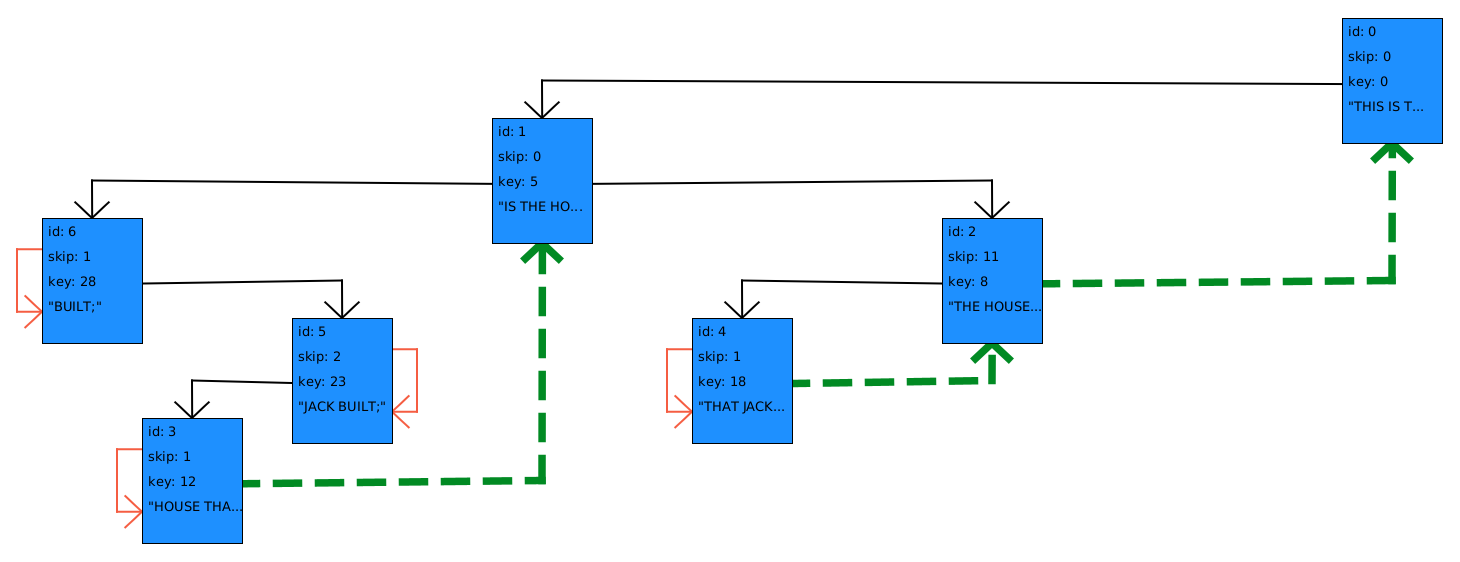
\includegraphics[width = \textwidth]{visaulRepresentation1.png}
    	\end{figure}
		
    	Główną klasą reprezentacji graficznej jest \emph{PatriciaTreeVisualRepresentation} w~paczce \emph{agh.jo.ui}. W implementacji głównej klasy i klas, z której korzysta, użyliśmy wtyczki (ang. \emph{plugin}) \emph{org.openjfx:javafx-maven-plugin:0.0.4} do \emph{Apache Maven 3.6.0}. Dodatkowo wykorzystaliśmy biblioteki \emph{org.openjfx:javafx-controls:13} oraz \emph{com.sirolf2009:fxgraph:0.0.3}. Rozszerzenia klas z tych bibliotek wykonaliśmy na podstawie przykładu podanego przez autora drugiej wymienionej biblioteki w popularnym serwisie \emph{StackOverflow} pod adresem \url{https://stackoverflow.com/questions/30679025/graph-visualisation-like-yfiles-in-javafx}.
		
		Reprezentacja graficzna była testowana manualnie na 7 przykładach struktury klasy \emph{PatriciaTree}. Część najciekawszych rezultatów testów manualnych została przedstawiona w postaci rysunków~ \ref{fig:PatriciaTreeVisualRepresentationTest1}, \ref{fig:PatriciaTreeVisualRepresentationTest2}, \ref{fig:PatriciaTreeVisualRepresentationTest3}, które znajdują się na następnej stronie.
		
        \begin{figure}[htb]
    		\caption{Przykładowa reprezentacja graficzna struktury klasy prostego przykładu \emph{PatriciaTree}, różniącego się od przykładu z~rysunku~\ref{fig:PatriciaTreeVisualRepresentation} jedynie wartościami parametrów wywołania konstruktora. Odmiennymi wartościami konstruktora klasy były: \emph{Encoding Encoding.JAVA} oraz \emph{WordStrategy WordStrategy.SINGLE}. Interpretacją wartości parametru konstruktora \emph{Encoding} jest fakt, iż klasa korzysta z~kodowania domyślnego \emph{JAVA} przy zamianie znaków na kod znaku i zamianie z kolei tego kodu na reprezentację binarną (o domyślnej długości bajtu równej 5 bitom). Interpretacją wartości parametru \emph{WordStrategy} jest przyjęcie strategii, gdzie klucz jest fragmentem pliku zaczynającego się w pozycji startowej klucza (przetrzymywanej w węźle drzewa w postaci pola \emph{key}) i kończącym się znakiem końca klucza, przed pozycją startową następnego klucza w pliku.}\label{fig:PatriciaTreeVisualRepresentationTest1}
    		\centering
    		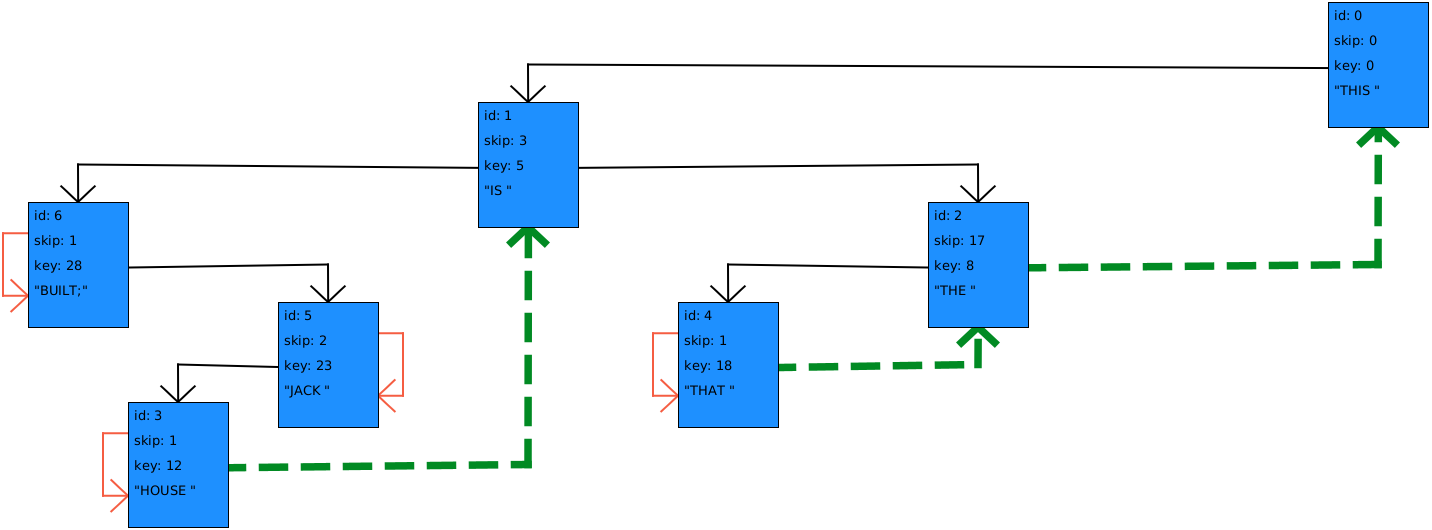
\includegraphics[width = \textwidth]{representationSmall_compressed.png}
    	\end{figure}
		
        \begin{figure}[htb]
    		\caption{Przykładowa reprezentacja graficzna struktury bardziej złożonego przykładu obiektu klasy \emph{PatriciaTree} różniącego się od przykładów przedstawionych na rysunkach~\ref{fig:PatriciaTreeVisualRepresentation} oraz~\ref{fig:PatriciaTreeVisualRepresentationTest1}. Widok przybliżony, przedstawia tą samą strukturę co rysunek~\ref{fig:PatriciaTreeVisualRepresentationTest3}.}\label{fig:PatriciaTreeVisualRepresentationTest2}
    		\centering
    		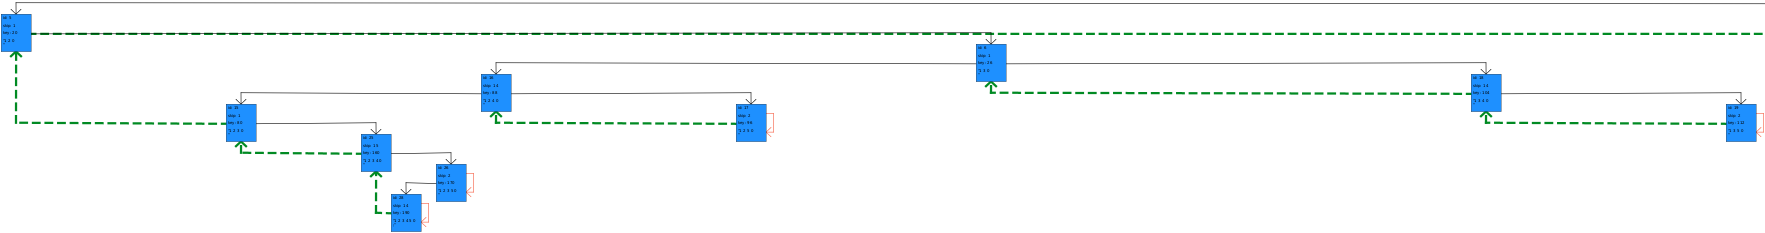
\includegraphics[width = \textwidth]{representationBigger-zoomedIn_compressed.png}
    	\end{figure}
    	
        \begin{figure}[htb]
    		\caption{Przykładowa reprezentacja graficzna struktury bardziej złożonego przykładu obiektu klasy \emph{PatriciaTree} różniącego się od przykładów przedstawionych na rysunkach \ref{fig:PatriciaTreeVisualRepresentation} oraz \ref{fig:PatriciaTreeVisualRepresentationTest1}. Widok oddalony, przedstawia tą samą strukturę co rysunek \ref{fig:PatriciaTreeVisualRepresentationTest2}.}\label{fig:PatriciaTreeVisualRepresentationTest3}
    		\centering
    		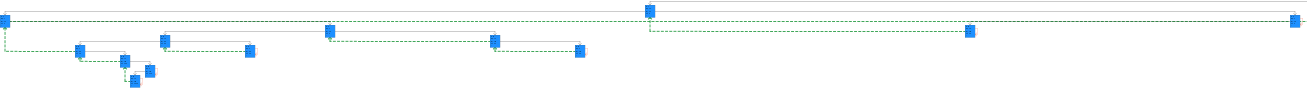
\includegraphics[width = \textwidth]{representationBigger-zoomedOut_compressed.png}
    	\end{figure}
		
		\section{Testy jednostkowe}\label{sec:czescPraktycznaRezultatyImplementacjiTestyJednostkowe}
		
    	Przez cały okres tworzenia i rozwijania autorskiej implementacji stopniowo dodawaliśmy testy jednostkowe pozwalające zweryfikować, czy nanoszone zmiany skutkowały spodziewanymi rezultatami. Mimo, że tworzenie ich zajęło nam bardzo dużo czasu, nie wyobrażam sobie, abyśmy bez nich byli w stanie znaleźć wiele pomyłek w naszym rozumowaniu, czy w tak efektywny sposób testować nasze podejrzenia co do trudniejszych do zrozumienia fragmentów algorytmów opisanych przez Knuth'a.
		
		Testy jednostkowe sprawdzają poprawność tworzonej struktury na różnych etapach, przy różnych konfiguracjach konstruktora klasy \emph{PatriciaTree} oraz na różnych przykładach plików źródłowych drzewa \emph{Patricia}. 
		
		W skład różnych testowanych etapów tworzenia struktury wchodzą między innymi: 
		\begin{enumerate}
		    \item Odczyt każdego ze znaków, 
		    \item Zamiana tego znaku na reprezentację binarną zgodną z wybranym kodowaniem,
		    \item Odczytywanie odpowiedniego fragmentu pliku zgodnie z przyjętą strategią.
		\end{enumerate}
		
		W skład testowanych konfiguracji konstruktora klasy \emph{PatriciaTree} wchodzą wszystkie możliwe kombinacje:
		\begin{enumerate}
		    \item Ilość bitów przyjętych dla symulowanej maszyny \emph{MIX},
		    \item Kodowanie znaków według tablicy znaków maszyny \emph{MIX} lub \emph{UTF-16},
		    \item Strategii: \emph{WordStrategy.SINGLE} lub \emph{WordStrategy.START\textunderscore POSITION \textunderscore TO\textunderscore EOF},
		    \item Różne kombinacje parametrów znaków \emph{charEOF} oraz \emph{charEOK},
		    \item Różne kombinacje konfiguracji konstruktora klasy \emph{CNFConverter}.
		\end{enumerate}
		
		W skład testowanych plików, na podstawie których tworzone są obiekty klasy \emph{PatriciaTree} wchodzi 7 plików źródłowych. Zawartość jednego z większych testowanych plików o rozmiarze 1.5 MB została przedstawiona fragmentem kodu źródłowego~\ref{prog:CNFsourceFile} oraz~\ref{prog:PatriciaSourceFile}. Drugi większy plik ma rozmiar 8.4 MB i na jego podstawie jest tworzony plik źródłowy drzewa \emph{Patricia}, którego zawartość przypomina plik w formacie \emph{DIMACS CNF}. Oznacza to, że plik wejściowy i wyjściowy konwertera różni się jedynie posortowanymi literałami wewnątrz klauzul, dodanym znakiem końca pliku ';', zamianą znaku końca linii na znak '\textbackslash n', brakiem linii komentarzy oraz linii problemu. Istnieje również trzeci plik w formacie \emph{DIMACS CNF} testujący współdziałanie klas \emph{CNFConverter} oraz \emph{PatriciaTree}, którego efektem jest reprezentacja wizualna z rysunków~\ref{fig:PatriciaTreeVisualRepresentationTest2} oraz~\ref{fig:PatriciaTreeVisualRepresentationTest3}. Dodatkowo stworzyliśmy 6 plików na podstawie zmodyfikowanego przykładu omawianego przez Knuth'a w swojej książce~\cite{KnuthsTheArtOfComputerProgramming3}. Treść tych plików wygląda następująco:
		\begin{enumerate}
		    \item \texttt{THIS IS THE HOUSE THAT JACK BUILT;}
		    \item \texttt{THIS$\Phi$IS$\Phi$THE$\Phi$HOUSE$\Phi$THAT$\Phi$JACK$\Phi$BUILT$\Phi\Pi$}
		    \item \texttt{THIS$\Phi$IS$\Phi\Phi$THE$\Phi$HOUSE$\Phi$THAT$\Phi$JACK$\Phi$BUILT$\Phi\Phi\Phi\Phi\Pi$ This Is Not A Part Of Any Key Because Of EOF Character $\Pi$}
		    \item \texttt{THIS $\Phi$IS $\Phi\Phi$THE $\Phi$HOUSE $\Phi$THAT $\Phi$JACK $\Phi$BUILT ;$\Phi\Phi\Phi\Phi\Pi$ This Is Not A Part Of Any Key Because Of EOF Character $\Pi$}
		    \item \texttt{THIS IS THE TEST FILE NUMBER 1 FOR DELETION ONE OF NODES. LONGESTWORDINTREE TODELETE. MORE NODES AFTER NODE TO DELETE;}
		    \item \texttt{THIS IS THE TEST FILE NUMBER 1 FOR DELETION ONE OF NODES. LONGESTWORDINTREExTODELETE. MORE NODES AFTER NODE TO DELETE;}
		\end{enumerate}
        
        Z dumą możemy powiedzieć, że wyżej omówione testy pokrywają następujący zakres klas, metod oraz linii kodu:
    
        \begin{enumerate}
            \item Względem głównej paczki (ang. \emph{package}) jaką jest \emph{agh.jo}:
                \subitem Pokrycie klas: 43\%,
                \subitem Pokrycie metod: 50\%,
                \subitem Pokrycie linii kodu: 45\%;
            \begin{enumerate}
                \item Względem paczki \emph{agh.jo.cnf.converter} (zawierającą klasy odpowiadające za przetwarzanie pliku w formacie .cnf):
                    \subitem Pokrycie klas: 100\%,
                    \subitem Pokrycie metod: 88\%,
                    \subitem Pokrycie linii kodu: 94\%;
                \item Względem paczki \emph{agh.jo.knuth} (zawierającą klasy związane ściśle z implementacją drzewa \emph{Patricia}):
                    \subitem Pokrycie klas: 100\%,
                    \subitem Pokrycie metod: 88\%,
                    \subitem Pokrycie linii kodu: 80\%;
                \item Względem paczki \emph{agh.jo.ui} (zawierającą klasy związane z reprezentacją graficzną struktury drzewa \emph{Patricia}):
                    \subitem Pokrycie klas: 0\%,
                    \subitem Pokrycie metod: 0\%,
                    \subitem Pokrycie linii kodu: 0\%;
                \item Względem paczki \emph{utils} (zawierającą klasy używane w wielu innych paczkach, na przykład te odpowiadające za obsługę klasy \emph{RandomAccessFile}):
                    \subitem Pokrycie klas: 60\%,
                    \subitem Pokrycie metod: 75\%,
                    \subitem Pokrycie linii kodu: 63\%.
            \end{enumerate}
        \end{enumerate}
	
    	\section{Instrukcja uruchomienie programu inżynierskiego}\label{sec:czescPraktycznaUruchamianieProgramu}
    	
    	Program inżynierski został napisany w sposób pozwalający na uruchomienie go w~kilku wariantach. Decyzja podziału na kilka wariantów uruchamiania spowodowana była długim czasem wykonywania i brakiem przejrzystości, gdy wszystkie warianty programu zostawały uruchomione jeden po drugim. 
    	
    	Uruchomienie podstawowej funkcjonalności programu odbywa się po przez przejście do folderu zawierającego foldery \emph{target} oraz \emph{src} i wpisaniu w konsoli komendy przedstawionej w postaci kodu źródłowego \ref{prog:runProgramJar}.
    	
    	\begin{program}
			\caption{Komenda pozwalającą uruchomić program w postaci pliku wykonywalnego \emph{jar} będąc w folderze zawierającym foldery \emph{target} oraz \emph{src}.}\label{prog:runProgramJar}
			\begin{lstlisting}[basicstyle=\small,]
java -jar target/TrieTreeImplementations_complete_standalone.jar RUN_MODE EXAMPLE_NUMBER OPTIONAL_DO_CONVERT_CNF_FILE
    	    \end{lstlisting}
	    \end{program}
    	
    	Zawartością folderu \emph{target} jest plik wykonywalny w formacie \emph{jar}. Konsekwencją zawarcia programu w postaci pliku wykonywalnego jest konieczność zawarcia dodatkowych plików, na których program przeprowadza operacje w oddzielnym folderze \emph{src/main/resources}. Są to pliki w formacie tekstowym o rozszerzeniu \emph{.cnf} lub \emph{.txt}. Pliki \emph{.cnf} są wykorzystywane przy konwersji ich do plików \emph{.txt}, które z kolei używane są do budowy struktury drzew \emph{Patricia} zawartych w postaci obiektów klasy \emph{PatriciaTree}.
    	
    	Komenda uruchamiająca plik wykonywalny, przedstawiona kodem źródłowym \ref{prog:runProgramJar} przyjmuje 3 parametry jako argumenty przedstawianego programu. 
    	\begin{enumerate}
    	    \item Pierwszym argumentem jest tryb w jakim chcielibyśmy uruchomić program - \texttt{RUN\textunderscore MODE}: 
    	        \subitem tekstowy -- dla którego wartość parametru powinna być równa \texttt{text};\newline
    	        Jest to tryb w którym informacje na temat drzewa przedstawiane są postaci tekstowej. Krótkie przykłady wyświetlają informacje o poszczególnych kluczach oraz prefiksach drzewa. Długie przykłady ze względu na czytelność tego rozwiązania nie robią tego. Oprócz tego, jeżeli dany przykład ma taką możliwość i zdecydujemy się na to, wyświetlana jest również informacja o dokonaniu konwersji pliku \emph{CNF} na plik źródłowy drzewa \emph{Patricia} (oczywiście przed jego stworzeniem).
    	        \subitem graficzny -- dla którego wartość parametru powinna być równa \texttt{visual};\newline
    	        Jest to tryb reprezentacji graficznej struktury drzewa zawartej w postaci obiektu klasy \emph{PatriciaTree}. Wykonuje on operacje opisane w trybie tekstowym oraz na ich koniec przedstawia użytkownikowi wizualizację stworzonego drzewa \emph{Patricia}.
    	   \item Drugim argumentem jest numer przykładu jaki chcielibyśmy, aby program przedstawił -- \texttt{EXAMPLE\textunderscore NUMBER}:
    	        \subitem Przyjmuje on jako swoje wartości liczby całkowite z zakresu od $0$ do $9$ odpowiadające indeksowi przykładu. \newline
    	        
            	Przykłady o numerach indeksów $5$ i $6$ są zbyt duże, aby obecna implementacja reprezentacji graficznej sobie z nimi poradziła, dlatego są one zabezpieczone wyjątkiem niepozwalającym na uruchomienie ich w trybie uruchomienia \texttt{visual}.
    	        \begin{enumerate}[label*=\arabic*.]
    	            \setcounter{enumii}{-1}
    	            \item Wartość \texttt{0} odpowiada przykładowi o indeksie $0$.
    	                \begin{enumerate}
    	                    \item Kodowanie znaków jest zgodne z kodowanie znaków w symulowanej maszynie \emph{MIX}.
    	                    \item Strategia pobierania kluczy definiująca czym jest znak jest równa \emph{START\textunderscore POSITION\textunderscore TO\textunderscore EOF}.
    	                    \item Nie zawiera pliku zawierającego koniunkcyjną postać normalną.
    	                    \item Zawartością pliku źródłowego obiektu klasy \emph{PatriciaTree} mu odpowiadającego jest: \newline
    	                ,,\texttt{THIS IS THE HOUSE THAT JACK BUILT;}``
    	                    \item Dodatkowo w pracy można zobaczyć wynik reprezentacji graficznej dla tego przykładu w postaci figury \ref{fig:PatriciaTreeVisualRepresentation}.
    	                \end{enumerate}
    	                
    	            \item Wartość \texttt{1} odpowiada przykładowi o indeksie $1$.
    	                \begin{enumerate}
    	                    \item Kodowanie znaków jest zgodne z kodowanie znaków w wirtualnej maszynie języka \emph{Java}.
    	                    \item Strategia pobierania kluczy definiująca czym jest znak jest równa \emph{SINGLE}.
    	                    \item Nie zawiera pliku zawierającego koniunkcyjną postać normalną.
    	                    \item Zawartością pliku źródłowego obiektu klasy \emph{PatriciaTree} mu odpowiadającego jest: \newline
    	                ,,\texttt{THIS IS THE HOUSE THAT JACK BUILT;}``
    	                    \item Dodatkowo w pracy można zobaczyć wynik reprezentacji graficznej dla tego przykładu w postaci figury \ref{fig:PatriciaTreeVisualRepresentationTest1}.
    	                \end{enumerate}
    	                
    	            \item Wartość \texttt{2} odpowiada przykładowi o indeksie $2$.
    	                \begin{enumerate}
    	                    \item Kodowanie znaków jest zgodne z kodowanie znaków w wirtualnej maszynie języka \emph{Java}.
    	                    \item Strategia pobierania kluczy definiująca czym jest znak jest równa \emph{SINGLE}.
    	                    \item Nie zawiera pliku zawierającego koniunkcyjną postać normalną.
    	                    \item Zawartością pliku źródłowego obiektu klasy \emph{PatriciaTree} mu odpowiadającego jest: \newline
    	                ,,\texttt{THIS$\Phi$IS$\Phi$THE$\Phi$HOUSE$\Phi$THAT$\Phi$JACK$\Phi$BUILT$\Phi\Pi$}``
    	                \end{enumerate}
    	                
    	            \item Wartość \texttt{3} odpowiada przykładowi o indeksie $3$.
    	                \begin{enumerate}
    	                    \item Kodowanie znaków jest zgodne z kodowanie znaków w wirtualnej maszynie języka \emph{Java}.
    	                    \item Strategia pobierania kluczy definiująca czym jest znak jest równa \emph{SINGLE}.
    	                    \item Nie zawiera pliku zawierającego koniunkcyjną postać normalną.
    	                    \item Zawartością pliku źródłowego obiektu klasy \emph{PatriciaTree} mu odpowiadającego jest: \newline
    	                ,,\texttt{THIS$\Phi$IS$\Phi\Phi$THE$\Phi$HOUSE$\Phi$THAT$\Phi$JACK$\Phi$BUILT$\Phi\Phi\Phi\Phi\Pi$ This Is Not A Part Of Any Key Because Of EOF Character $\Pi$}``
    	                \end{enumerate}
    	                
    	            \item Wartość \texttt{4} odpowiada przykładowi o indeksie $4$.
    	                \begin{enumerate}
    	                    \item Kodowanie znaków jest zgodne z kodowanie znaków w wirtualnej maszynie języka \emph{Java}.
    	                    \item Strategia pobierania kluczy definiująca czym jest znak jest równa \emph{SINGLE}.
    	                    \item Nie zawiera pliku zawierającego koniunkcyjną postać normalną.
    	                    \item Zawartością pliku źródłowego obiektu klasy \emph{PatriciaTree} mu odpowiadającego jest: \newline
    	                ,,\texttt{THIS $\Phi$IS $\Phi\Phi$THE $\Phi$HOUSE $\Phi$THAT $\Phi$JACK $\Phi$BUILT ;$\Phi\Phi\Phi\Phi\Pi$ This Is Not A Part Of Any Key Because Of EOF Character $\Pi$}``
    	                \end{enumerate}
    	                
    	            \item Wartość \texttt{5} odpowiada przykładowi o indeksie $5$.
    	                \begin{enumerate}
    	                    \item Kodowanie znaków jest zgodne z kodowanie znaków w wirtualnej maszynie języka \emph{Java}.
    	                    \item Strategia pobierania kluczy definiująca czym jest znak jest równa \emph{SINGLE}.
    	                    \item Plik zawierający koniunkcyjną postać normalną ma rozmiar 1,5 Mb, a~fragment jego zawartości przedstawia kod źródłowy \ref{prog:CNFsourceFile}.
    	                    \item Plik źródłowy obiektu klasy \emph{PatriciaTree} ma rozmiar 1,5 Mb, a jego fragment przestawia kod źródłowy \ref{prog:PatriciaSourceFile}.
    	                \end{enumerate}
    	                
    	            \item Wartość \texttt{6} odpowiada przykładowi o indeksie $6$.
    	                \begin{enumerate}
    	                    \item Kodowanie znaków jest zgodne z kodowanie znaków w wirtualnej maszynie języka \emph{Java}.
    	                    \item Strategia pobierania kluczy definiująca czym jest znak jest równa \emph{SINGLE}.
    	                    \item Plik zawierający koniunkcyjną postać normalną ma rozmiar 8,4 Mb, a~jego zawartość przypomina strukturę pliku \emph{CNF} przykładu o indeksie $5$.
    	                    \item Plik źródłowy obiektu klasy \emph{PatriciaTree} ma rozmiar 8,4 Mb, a jego zawartość jest zbliżona do zawartości pliku \emph{CNF} tego przykładu (o indeksie $6$). Rozróżnia go zakończenie każdej linii w postaci znaku '\textbackslash n', znak końca pliku postaci znaku ';', posortowane literały w każdej z klauzul oraz brak linii komentarzy oraz linii problemu.
    	                \end{enumerate}
    	                
    	            \item Wartość \texttt{7} odpowiada przykładowi o indeksie $6$.
    	                \begin{enumerate}
    	                    \item Kodowanie znaków jest zgodne z kodowanie znaków w wirtualnej maszynie języka \emph{Java}.
    	                    \item Strategia pobierania kluczy definiująca czym jest znak jest równa \emph{SINGLE}.
    	                    \item Plik zawierający koniunkcyjną postać normalną ma rozmiar 532 bajtów, a~jego zawartość przypomina strukturę innych plików \emph{CNF} (z przykładów o indeksie $5$ i $6$).
    	                    \item Plik źródłowy obiektu klasy \emph{PatriciaTree} ma rozmiar 203 bajtów, a jego zawartość jest zbliżona do zawartości pliku \emph{CNF} tego przykładu (o indeksie $7$). \newpage Rozróżnia go zakończenie każdej linii w postaci znaku '\textbackslash n', znak końca pliku postaci znaku ';', posortowane literały w każdej z klauzul oraz brak linii komentarzy oraz linii problemu.
    	                    \item Dodatkowo w pracy można zobaczyć wynik reprezentacji graficznej dla tego przykładu w postaci figur \ref{fig:PatriciaTreeVisualRepresentationTest2} i \ref{fig:PatriciaTreeVisualRepresentationTest3}.
    	                \end{enumerate}
    	                
    	            \item Wartość \texttt{8} odpowiada przykładowi o indeksie $8$.
    	                \begin{enumerate}
    	                    \item Kodowanie znaków jest zgodne z kodowanie znaków w wirtualnej maszynie języka \emph{Java}.
    	                    \item Strategia pobierania kluczy definiująca czym jest znak jest równa \emph{SINGLE}.
    	                    \item Nie zawiera pliku zawierającego koniunkcyjną postać normalną.
    	                    \item Zawartością pliku źródłowego obiektu klasy \emph{PatriciaTree} mu odpowiadającego jest: \newline
    	                ,,\texttt{THIS IS THE TEST FILE NUMBER 1 FOR DELETION ONE OF NODES. LONGESTWORDINTREE TODELETE. MORE NODES AFTER NODE TO DELETE;}``
    	                    \item Dodatkowo w pracy można zobaczyć wynik reprezentacji graficznej dla tego przykładu w postaci figury \ref{fig:Delete1}.
    	                \end{enumerate}
    	                
    	            \item Wartość \texttt{9} odpowiada przykładowi o indeksie $9$.
    	                \begin{enumerate}
    	                    \item Kodowanie znaków jest zgodne z kodowanie znaków w wirtualnej maszynie języka \emph{Java}.
    	                    \item Strategia pobierania kluczy definiująca czym jest znak jest równa \emph{SINGLE}.
    	                    \item Nie zawiera pliku zawierającego koniunkcyjną postać normalną.
    	                    \item Zawartością pliku źródłowego obiektu klasy \emph{PatriciaTree} mu odpowiadającego jest: \newline
    	                ,,\texttt{THIS IS THE TEST FILE NUMBER 1 FOR DELETION ONE OF NODES. LONGESTWORDINTREExTODELETE. MORE NODES AFTER NODE TO DELETE;}``
    	                    \item Dodatkowo w pracy można zobaczyć wynik reprezentacji graficznej dla tego przykładu w postaci figury \ref{fig:Delete2}.
    	                \end{enumerate}
    	        \end{enumerate}
    	    \item Trzecim argumentem jest opcjonalny argument decydujący o tym czy przed stworzeniem obiektu klasy \emph{PatriciaTree} chcielibyśmy wykonać konwersję pliku \emph{CNF} na źródłowy dla naszego obiektu -- \texttt{OPTIONAL\textunderscore DO\textunderscore CONVERT\textunderscore CNF\textunderscore FILE}. Przyjmuje wartość \texttt{true} lub \texttt{false}. \newline 
    	    
    	    Pliki źródłowe obiektów klasy \emph{PatriciaTree} dla wszystkich przykładów są stworzone przed uruchomieniem programu. Nie należy ich kasować. Można wykasować ich zawartość. Są one nadpisywane w przypadku, gdy argument ten przyjmuje wartość \texttt{true}. Gdy nie zostanie podany ten parametr, domyślną przyjmowaną wartością jest \emph{false} wewnątrz programu.
    	\end{enumerate}
	\chapter{Podsumowanie}\label{cha:podsumowanie}
	
	\section{Osiągnięcia}\label{sec:PodsumowanieZaslugi}
	
	\begin{enumerate}
	    \item Bazując na książce ,,Sztuka programowania`` Donalda E. Knuth'a~\cite{KnuthsTheArtOfComputerProgramming3} w wersji angielskiej oraz posiłkując się wersją polską, przedstawienie -- w przystępnej formie -- głównych konceptów wykraczających poza zakres rozdziału ,,Przeszukiwanie cyfrowe`` i ćwiczeń go dotycz dotyczących.
	    
	    \item Dokładna analiza tematów nie poruszanych przez Donalda E. Knuth'a, wykorzystująca ponad 30 źródeł w języku polskim, bądź angielskim.
	    
	    \item Implementacja parametryzowanej klasy \emph{MixMachine} symulującej reprezentację binarną i kodowanie znaków maszyny \emph{MIX}.
	    
	    \item Implementacja drzewa \emph{Patricia}, według algorytmów opisanych przez Donalda Knuth'a~\cite{KnuthsTheArtOfComputerProgramming3} w postaci parametryzowanej klasy \emph{PatriciaTree}.
	    
	        \begin{enumerate}
	            \item Implementacja operacji \emph{look-up} oraz \emph{search} w kontekście prefiksów oraz \emph{insert} na klasie \emph{PatriciaTree}. Wykonanie na podstawie opisu Knuth'a.
	        \end{enumerate}
	    
	    \item Implementacja drzewa \emph{Patricia}, wykorzystującej odmienny sposób reprezentacji kluczy od opisanego przez Knuth'a, za pomocą wzorca projektowego strategia w~postaci sparametryzowanej klasy \emph{FileOps}.
	    
	        \begin{enumerate}
	            \item Implementacja operacji \emph{look-up} oraz \emph{search} w kontekście kluczy  oraz \emph{insertAll} na klasie \emph{PatriciaTree}. Wykonanie na podstawie wcześniej zaimplementowanych operacji dotyczących prefiksów.
	        \end{enumerate}
	    
	    \item Implementacja konwertera plików \emph{DIMACS CNF} -- w postaci parametryzowanej klasy \emph{CNFConverter} -- na format plików źródłowych potrzebnych do utworzenia obiektów klasy \emph{PatriciaTree}.
	    
	    \item Implementacja ponad 570 złożonych testów jednostkowych sprawdzających poprawność tworzonych obiektów klas \emph{PatriciaTree}, \emph{CNFConverter} oraz innych klas przez nie wykorzystywanych.
	    
	    \item Implementacja reprezentacji graficznej stworzonej struktury drzewa \emph{Patricia}, w~postaci klasy \emph{PatriciaTreeVisualization}.
	    
	    \item Implementacja głównej klasy programu \emph{App} obsługującej argumenty uruchomienia pliku wykonywalnego, oraz automatyzacja przygotowania pliku wykonywalnego za pomocą narzędzia \emph{Maven}.
	    
	    \item Testy manualne ponad 9 złożonych przykładów reprezentacji graficznej oraz głównej klasy programu \emph{App} na 2 różnych platformach systemowych (\emph{Unix} oraz \emph{Windows}).
	\end{enumerate}
	
	\section{Rezultaty implementacji oraz analiza pracy}\label{sec:czescPraktycznaRezultatyImplementacji}
	
	Implementacje uważamy za udaną. Udało się nam zaimplementować algorytm opisany z myślą o innym, nisko poziomowym języku, maszynie posiadającej kompletnie inną tablicę znaków oraz inną reprezentację binarną. Dodatkowo rozszerzyliśmy ten algorytm dla przypadków ogólnych -- w postaci strategii pojedynczego słowa. Wykorzystanie implementacji w rozwiązaniu problemu koniunkcyjnej postaci normalnej przebiega zgodnie z postawionymi, podstawowymi założeniami. Reprezentacja graficzna spełnia swoją rolę obrazowania struktury stworzonego drzewa \emph{Patricia}. Testy jednostkowe potwierdzają poprawność wprowadzanych zmian do implementacji.
	
	Mając to wszystko na uwadze, oczywiście nie obyło się bez swojego rodzaju założeń upraszczających. Zakres programu projektowego ze względu na jego możliwości jest bardzo szeroki i można odnieść wrażenie, że zaczyna on wiele różnych tematów nie doprowadzając ich do zwieńczenia. W związku z tym w wielu miejscach pojawiają się koncepcje upraszczające, bądź porzucenie pewnych funkcjonalności na rzecz rozwinięcia innych. Oczywiście można też w tym miejscu zauważyć okazję do kontynuowania tego tematu, poszerzania wglądu i swojego wkładu do niego.
	
		\subsection{Implementacja drzewa \emph{Patricia} według Knuth'a}\label{sec:RezultatyImplementacjiDrzewaPatriciaKnuth}
		
		Zgodnie z tym co opisaliśmy w poprzedniej sekcji cała zaimplementowana funkcjonalność klasy \emph{PatriciaTree} jest udana pod względem poprawności i prędkości przetwarzania dużej ilości danych. 
		
		Oczywiście, aby w pełni stwierdzić czy implementacja jest optymalna należałoby porównać ją do innych implementacji przy użyciu testów wydajnościowych pamięciowych i czasu wykonywania. Na pewno również w kontekście specyfikacji samego języka \emph{Java} dałoby się zoptymalizować pewnie działania.
		
		W autorskiej implementacji drzewa \emph{Patricia} brakuje kilku operacji opisanych w~części teoretycznej. Takimi operacjami są: usuń (ang. \emph{delete}), poprzednik (ang. \emph{predecessor}), następca (ang. \emph{successor}), minimum oraz maksimum. 
		
		Do samej budowy drzewa oraz jego przeszukiwania w kontekście odnajdywania prefiksów i kluczy, na których skupiamy się w niniejszej pracy, wymienione wyżej operacje są niepotrzebne. \newpage Z powodu zaplanowanego zakresu pracy inżynierskiej pominęliśmy ich implementację. Plan pracy nigdy nie przewidywał implementacji wszystkich możliwych do przeprowadzenia działań na drzewie. Dodatkowo Knuth nie opisuje nawet w swoich ćwiczeniach oraz rozwiązaniach algorytmu tych operacji. Nie pojawiają się one nawet w~formie nawiązania czy wspomnienia o nich.
		
		Szczególnie skomplikowaną do zaimplementowania metodą okazuje się metoda usuwania klucza. W obecnej implementacji należałoby rozróżnić dwa możliwe rozwiązania algorytmu usuwania klucza z drzewa. 
		
		Pierwszym rozwiązaniem jest usuwanie jedynie węzła ze struktury drzewa, pozostawiając plik nienaruszony. Wiązałoby by się to jednak z przebudową całego pod-drzewa węzła usuniętego, a potencjalnie mogłoby by to wymagać modyfikacji również struktury węzłów wychodzący poza to pod-drzewo -- ze względu na dowiązania węzłów do ich przodków.
		
		Drugim rozwiązaniem jest usuwanie klucza z pliku, z czym wiązałoby się przesunięcie całej zawartości pliku w lewo o $d$ znaków (w przedstawionej implementacji bajtów odpowiadających $d$ znakom) od miejsca w którym zaczynał się usunięty klucz. Konsekwencją takiego zabiegu byłaby zmiana pozycji startowej klucza zawarta we wszystkich węzłach reprezentujące klucze właśnie zaczynające się po pozycji startowej wykasowanego klucza. Struktura drzewa \emph{Patricia} nie pozwala na łatwe znalezienie węzłów zaczynających się po określonej pozycji, a więc musielibyśmy sprawdzić wszystkich węzły lub wyłuskiwać każdy węzeł ze względu na jego klucz -- co byłoby skomplikowane ze względu na fakt, że bylibyśmy w trakcie modyfikacji drzewa.
		
		Rysunki \ref{fig:Delete1} i \ref{fig:Delete2} przedstawiają różnicę między drzewami \emph{Patricia}, z których drzewo \ref{fig:Delete1} zawiera węzeł z dodatkowym kluczem, a drzewo \ref{fig:Delete2} nie zawiera tego węzła. Ma to na celu obrazować uproszczony wpływ wykasowania węzła ze struktury drzewa. Efekt taki uzyskany został poprzez stworzenie dwóch źródłowych plików dla obiektów klasy \emph{PatriciaTree}, które różnią się jedynie fragmentem określającym istnienie dodatkowego klucza lub jego brak. Fragment ten ma postać w przypadku drzewa z rysunku \ref{fig:Delete1} ,,\texttt{LONGESTWORDINTREE TODELETE. }``, a w przypadku drzewa z rysunku \ref{fig:Delete2} ,,\texttt{LONGESTWORDINTREExTODELETE. }``. Różnica w tych dwóch fragmentach jest subtelna, ale znacząca. Poprzez zmianę znaku spacji na znak 'x' dwa klucze z rysunku \ref{fig:Delete1} stały się jednym kluczem na rysunku \ref{fig:Delete2}. Dzięki tym ilustracją możemy zaobserwować jak duży wpływ na strukturę drzewa może mieć operacja usunięcia jednego węzła -- nawet przyjmując upraszczające założenia.\newpage
    	
        \begin{figure}[htb]
    		\caption{Wizualizacja obiektu klasy \emph{PatriciaTree} stworzonego na podstawie pliku o zawartości ,,\texttt{THIS IS THE TEST FILE NUMBER 1 FOR DELETION ONE OF NODES. LONGESTWORDINTREE TODELETE. MORE NODES AFTER NODE TO DELETE;}``. Węzeł oznaczony liczbą 1 jest węzłem reprezentującym klucz ,,\texttt{LONGESTWORDINTREE }``. Węzeł oznaczony liczbą 2 jest węzłem reprezentującym klucz ,,\texttt{TODELETE. }``. Węzeł oznaczony liczbą 3 jest węzłem reprezentującym klucz ,,\texttt{TO }``.}\label{fig:Delete1}
    		\centering
    		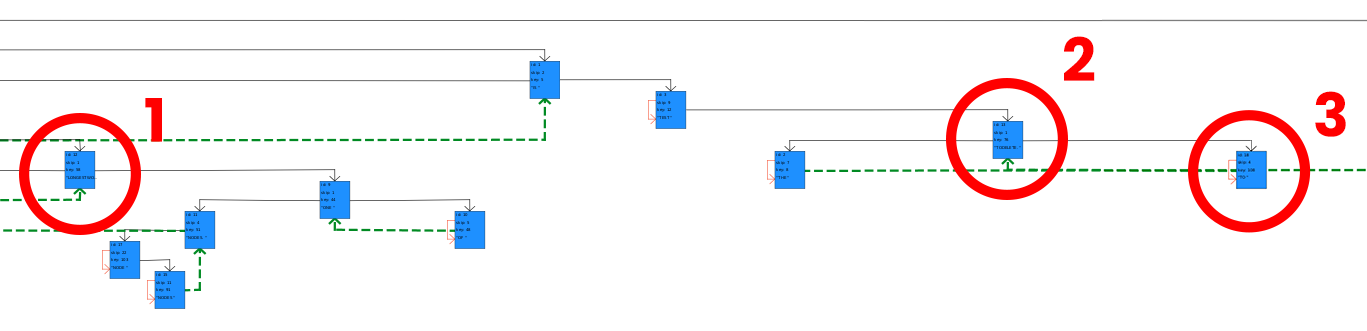
\includegraphics[width = \textwidth]{Delete1.png}
    	\end{figure}
    	
        \begin{figure}[htb]
    		\caption{Wizualizacja obiektu klasy \emph{PatriciaTree} stworzonego na podstawie pliku o zawartości ,,\texttt{THIS IS THE TEST FILE NUMBER 1 FOR DELETION ONE OF NODES. LONGESTWORDINTREExTODELETE. MORE NODES AFTER NODE TO DELETE;}``. Węzeł oznaczony liczbą 1 jest węzłem reprezentującym klucz ,,\texttt{LONGESTWORDINTREExTODELETE. }``. Węzeł oznaczony liczbą 3 jest węzłem reprezentującym klucz ,,\texttt{TO }``.}\label{fig:Delete2}
    		\centering
    		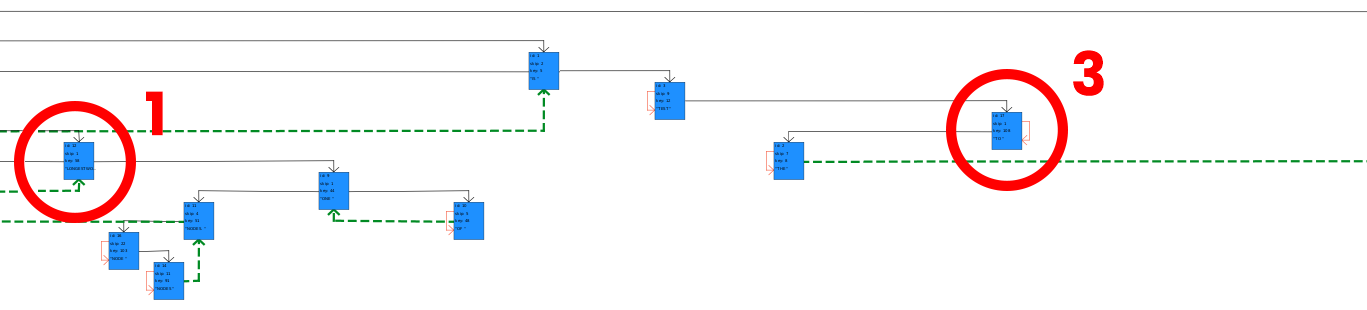
\includegraphics[width = \textwidth]{Delete2.png}
    	\end{figure}
		
		Knuth podczas omawiania algorytmów drzewa \emph{Patricia} wspomina jeszcze o możliwości dodawania nowych kluczy na końcu pliku poprzez wyznaczanie nowego unikatowego znaku końca pliku, który zamiast pojedynczego znaku miałby być starym znakiem końca pliku poprzedzonym liczbą tworzącym unikatowy ciąg znaków. Ta operacja również nie została zaimplementowana. Możliwe, że da się osiągnąć taki sam efekt w bardziej elegancki sposób. 
		
		\subsection{Autorska modyfikacja algorytmu drzewa \emph{Patricia}}\label{sec:RezultatyImplementacjiDrzewaPatriciaAutorska} 
	    
	    Odpowiedzią na tezę tego projektu inżynierskiego jest implementacja drzewa \emph{Patricia} w postaci klasy \emph{PatriciaTree} oraz możliwość wyboru strategii interpretacji tego czym jest klucz, dzięki parametrowi konstruktora typu \emph{enum} przyjmującym jedną z dwóch wartości: \emph{WordStrategy.START\textunderscore POSITION\textunderscore TO\textunderscore EOF} (odpowiadającej interpretacji Knuth'a tego czym jest klucz) lub \emph{WordStrategy.SINGLE} (mojej interpretacji, gdzie w skład każdego klucza nie wchodzą wszystkie klucze występujące po nim w pliku). 
	    
	    Zgodnie z opisem w sekcji~\ref{sec:czescPraktycznaImplementacjaDrzewaPatriciaAutorska}, modyfikacja algorytmów Donalda Knuth'a dotyczących drzewa \emph{Patricia} powiodła się. Dzięki dodaniu parametrów typu \emph{char} konstruktora klasy \emph{PatriciaTree}, określającego znak końca klucza modyfikacja ograniczała się w praktyce do stworzenia klasy implementującej oddzielny algorytm odczytywania klucza z pliku.
	    
	    Sprawdzenie rezultatów poprawności algorytmów wykonaliśmy za pomocą testów jednostkowych, opisanych w sekcji~\ref{sec:czescPraktycznaRezultatyImplementacjiTestyJednostkowe}. 
	    
	    Jednym z dowodów na brak znacznych modyfikacji względem algorytmów Knuth'a oraz struktury drzewa jest fakt, iż obie interpretacje tego czym jest klucz są dostępne w~jednej klasie \emph{PatriciaTree} -- a wybór ich odbywa się za pomocą wzorca projektowego strategia, który dostarcza jedną z klas dziedziczących po klasie \emph{FileOpsStrategy}. 
	    
	    Drugim dowodem na nieznaczny wpływ modyfikacji interpretacji tego czym jest klucz jest reprezentacja graficzna. Przykładowymi rysunkami przedstawiającymi przykład reprezentacji graficznej struktury drzewa dla takiej samej zawartości plików, ale różnej strategii pobierania klucza z pliku (interpretacji tego czym jest klucz) są rysunki ~\ref{fig:PatriciaTreeVisualRepresentation} i~\ref{fig:PatriciaTreeVisualRepresentationTest1}. 
	    
	    Dodatkową własnością, którą można zaobserwować na tych rysunkach jest fakt -- iż mimo oprócz różnych strategii te dwa obiekty korzystają z różnych kodowań znaków i~reprezentacji binarnych -- to struktura drzewa nie zmienia się w sposób znaczący. Różnicę w strukturze drzewa spowodowaną przez kodowanie znaków można zaobserwować dopiero na znakach wymagający do ich reprezentacji różnej ilości bajtów. Przykładami takich znaków są: $\theta$, $\Phi$, $\Pi$.
		
		\subsection{Koniunkcyjna postać normalna -- wykorzystanie autorskiej implementacji w rozwiązaniu problemu praktycznego}\label{sec:czescPraktycznaRezultatyCNF}
		
		Implementacja konwertera plików w formacie \emph{DIMCAS CNF} wykorzystuje klasę \emph{RandomAccessFile}, której obsługa została już napisana i wykorzystana wcześniej w programie projektowym. Niestety prędkość konwertowania pliku nie jest zadowalająca i może być to spowodowane właśnie wyborem klasy obsługującej pracę na plikach. Możliwe, że użycie kombinacji klas \emph{File}, \emph{FileReader}, \emph{BufferedReader} przez klasę \emph{CNFReader} (a przez klasę \emph{CNFWriter}: \emph{File}, \emph{FileWriter}, \emph{BufferedWriter}) skutkowałoby szybszym przetwarzaniem plików.
		
		Przykłady struktury klasy \emph{PatriciaTree} z klasy \emph{agh.jo.Examples} mają możliwość nie konwertowania plików poprzez ustawienie finalnego, statycznego pola \emph{DEFAULT\textunderscore IS\textunderscore DO\textunderscore CONVERT\textunderscore CNF\textunderscore SOURCE\textunderscore FILE\textunderscore TO\textunderscore PATRICIA\textunderscore SOURCE\textunderscore FILE} klasy \emph{App} na wartość \emph{false} dla przypadków kiedy nie nastąpiła zmiana pliku źródłowego \emph{CNF} i parametrów konstruktów klas \emph{PatriciaTree} i \emph{CNFConverter}.\newpage
		
		Jednym z wcześniej wspomnianych założeń upraszczających było założenie przyjęte przy konwertowaniu plików w formacie \emph{DIMACS CNF} dotyczące togo, że nie mogą się w nich pojawić dwie identyczne klauzule z punktu widzenia logiki Bool'a. Dzięki temu konwerter nie musi sprawdzać, czy klauzula wstawiana do pliku źródłowego drzewa już w~nim nie występuje. W efekcie implementacja drzewa \emph{Patricia} wyrzuca wyjątek mówiący o tym, że do struktury nie może zostać wstawiony klucz będący prefiksem już istniejącego~klucza.
		
		Kolejnym założeniem uproszczającym jest to, że każda klauzula w pliku \emph{DIMACS CNF} kończy się znakiem (lub kombinacją znaków) końca linii. Specyfikacja plików w~tym formacie mówi o przypadkach, w których może się zdarzyć, że dwie klauzule są w~tej samej linii, a rozdziela je ciąg znaków \emph{klauzula1 + `` 0 `` + klauzula2}. Specyfikacja mówi również o nieregularnych przypadkach, gdzie ostatnia klauzula w pliku nie jest zakończona kombinacją znaków \emph{ostatnia\textunderscore klauzula + `` 0``}. Dodatkowo dopuszczane są przypadki, w~których linie komentarzy przeplatają się z liniami klauzul.
		
		Następnym założeniem uproszczającym, niezwiązanym już ze specyfikacją plików w formacie \emph{DIMACS CNF}, jest wymóg klasy \emph{CNFConverter} istnienia pliku wejściowego i wyjściowego konwertera. Podobnie klasa \emph{PatriciaTree} wymaga istnienia pliku wejściowego, który jest plikiem wyjściowym konwertera. Zapobiega to sytuacji, w~której użytkownik mógłby popełnić błąd podając inne ścieżki czy nazwy plików dla tych dwóch klas i mógłby stanąć on przed zagadką ,,Dlaczego skoro konwerter poprawnie działa to klasa drzewa \emph{Patricia} wyrzuca wyjątek związany z brakiem pliku, który przecież konwerter \emph{NA PEWNO} tworzy? ``. Oczywiście nigdy się nie zdarzyło tak, żeby użytkownikiem w~takim scenariuszu byli autorzy tej pracy inżynierskiej -- czyli my.
		
		Z kolei wnioskiem wynikającym z zastosowania struktury jaką jest drzewo \emph{Patricia} do problemu plików zawierających koniunkcyjną postać normalną jest fakt, że nie jest ona kompatybilna z problemem. Drzewa typu \emph{Trie} korzystają z własności wynikających z kolejności ciągów znaków, podczas gdy klauzula, która jest alternatywą literałów -- nie dba o kolejność literałów. Dlatego do problemu, w którym kolejność wartości nie ma znaczenia lepszym wyborem były by \emph{hashowe}-funkcje (ang. \emph{hash-functions}). Inspiracją dla tego rozwiązania było przedstawienie ich praktycznego wykorzystania w wideo-artykule na przykładzie aplikacji \emph{Shazam} (aplikacji znajdującej nazwę utworu muzycznego na podstawie jego fragmentu rozpoznanego przez mikrofon telefonu) przez kanał \emph{RealEngineering} na \emph{YouTube}~\cite{HashFunctionsShazamYoutubeRealEngineering}.
		
		Dodatkowym problem, który dla ułatwienia ignorujemy jest fakt, że z logicznego punktu widzenia drzewa typu \emph{Trie} są alternatywą kluczy w nim w zawartych, podczas gdy koniunkcyjna postać normalna jest koniunkcją klauzul. Bardziej nadającym się do tego rozwiązania -- z tego punktu widzenia -- problemem jest problem \emph{DNF} (dysjunkcyjna postać normalna), który jest alternatywą koniunkcji literałów. \newpage Nie rozwiązuję to jednak problemu jakim jest dowolność kolejności literałów w~klauzulach alternatyw czy koniunkcji literałów.
		
		\subsection{Reprezentacja graficzna stworzonego drzewa}\label{sec:czescPraktycznaRezultatyImplementacjiReprezentacja graficzna}
		
		Dodanie reprezentacji graficznej jako dodatkowego elementu edukacyjnego oraz testowego zakończyło się sukcesem. Niekonwencjonalna budowa drzewa \emph{Patricia} -- a dokładniej -- orientacja węzłów względem siebie i gałęzi obrazujących relację tych węzłów -- wymagała autorskiej implementacji tworzenia wizualnej struktury drzewa. Niestety wymagało to dodania dodatkowych ,,ukrytych`` węzłów na gałęziach drzewa, aby było zrozumiałe z którego węzła wychodzi dana krawędź i do którego wchodzi. Spowodowało to, że obecnie zaimplementowana funkcjonalność przesuwania węzłów drzewa \emph{Patricia} w~czasie działania programu nie spełnia swojej funkcji, gdyż gałęzie zostają w pozycji startowej i niestety zaburza ona czytelność grafu. Decyzję czy warto reorganizować położenie węzłów drzewa \emph{Patricia} na grafie pozostawiam użytkownikowi.
		
		Jedynym ograniczeniem wizualizacji struktury klasy \emph{PatriciaTree} jest ilość krawędzi w drzewie -- bo na tym etapie przetwarzania program nie daje sobie rady z ilością wymaganej pamięci. Klasa \emph{PatriciaTreeVisualization} nie jest w stanie sobie poradzić ze strukturami klasy \emph{PatriciaTree} stworzonej na podstawie dwóch dużych plików o rozmiarze 1.5 i 8.4 Mb. Jest to dosyć ciekawy problem, którego rozwiązaniem nie może być po prostu zwiększenie ilości pamięci RAM przydzielonej programowi, gdyż zawsze może istnieć większy przykład drzewa \emph{Patricia}, wymagający większej ilości pamięci RAM. Rozwiązaniem tego problemu mogłoby być dynamiczne tworzenie i kasowanie obiektów odpowiednio widocznych i nie widocznych obecnie na ekranie oraz ograniczenie obszaru jaki może widzieć użytkownik korzystając z funkcjonalności oddalenia widoku. Inspiracją tego rozwiązania jest rozwiązanie popularnie stosowane w dzisiejszych grach, gdzie jedynie obiekty widoczne w następnej klatce są renderowane, a stare obiekty są niszczone na rzecz wolnej pamięci.
		
	\section{Możliwości rozwoju}\label{sec:podsumowanieMozliwosciRozwoju}
	
	Implementacja wykonana w zakresie tego projektu inżynierskiego w formie klasy \emph{PatriciaTree} jest uniwersalna i nadaje się do zastosowania przy problemach dużych zbiorów, których elementy mają określoną kolejność -- są ciągami liczb czy innych znaków. 
	
	Możliwością rozwoju samej implementacji postaci klasy \emph{PatriciaTree} jest implementacja operacji pominiętych w obecnej wersji (usuń, następca, poprzednik, minimum, maksimum). Dodatkowo można rozwinąć projekt o algorytmy umożliwiające modyfikację pliku źródłowego drzewa \emph{Patricia}. Takim algorytmem może być na przykład algorytm dodawania lub usuwania - do drzewa i jednocześnie pliku -- nowego klucza. Dokładniej opisany został ten problem w sekcji~\ref{sec:RezultatyImplementacjiDrzewaPatriciaKnuth}.
	
	Rozwojem rozważań tematu dotyczącego koniunkcyjnej postaci normalnej może być próba zastosowania \emph{hash}-funkcji do szybszego przeszukiwania zbioru klauzul. Dokładniej problem ten opisałem w sekcji~\ref{sec:czescPraktycznaRezultatyCNF}.
	
	Kolejną okazją do rozwoju tego projektu jest modyfikacja implementacji reprezentacji graficznej tak, aby niezależnie od rozmiaru drzewa \emph{Patricia}, generacja wizualnej warstwy projektu zawsze kończyła się sukcesem. Opis propozycji rozwiązania tego problemu opisałem w sekcji~\ref{sec:czescPraktycznaRezultatyImplementacjiReprezentacja graficzna}.
	
	%Kod poniżej dodaje Bibliografię do spisu treści
	\cleardoublepage{}
	\phantomsection{}
	\addcontentsline{toc}{chapter}{Bibliografia}
	\printbibliography{}
	
	% Załączniki
	\begin{appendices}
		\makeatletter% Kod poniżej powoduje ustęp w spisie treści
		\addtocontents{toc}{\let\protect\l@chapter\protect\l@section}
		
		%\input{knuth}
		\renewcommand\thesection{\Alph{section}}
\renewcommand\thefigure{\thesection.\arabic{figure}}
\setcounter{section}{1}
\setcounter{figure}{0}
\begin{figure}
		\centering
		\caption{Diagram klas paczki agh.jo.knuth}\label{fig:classDiagram}
		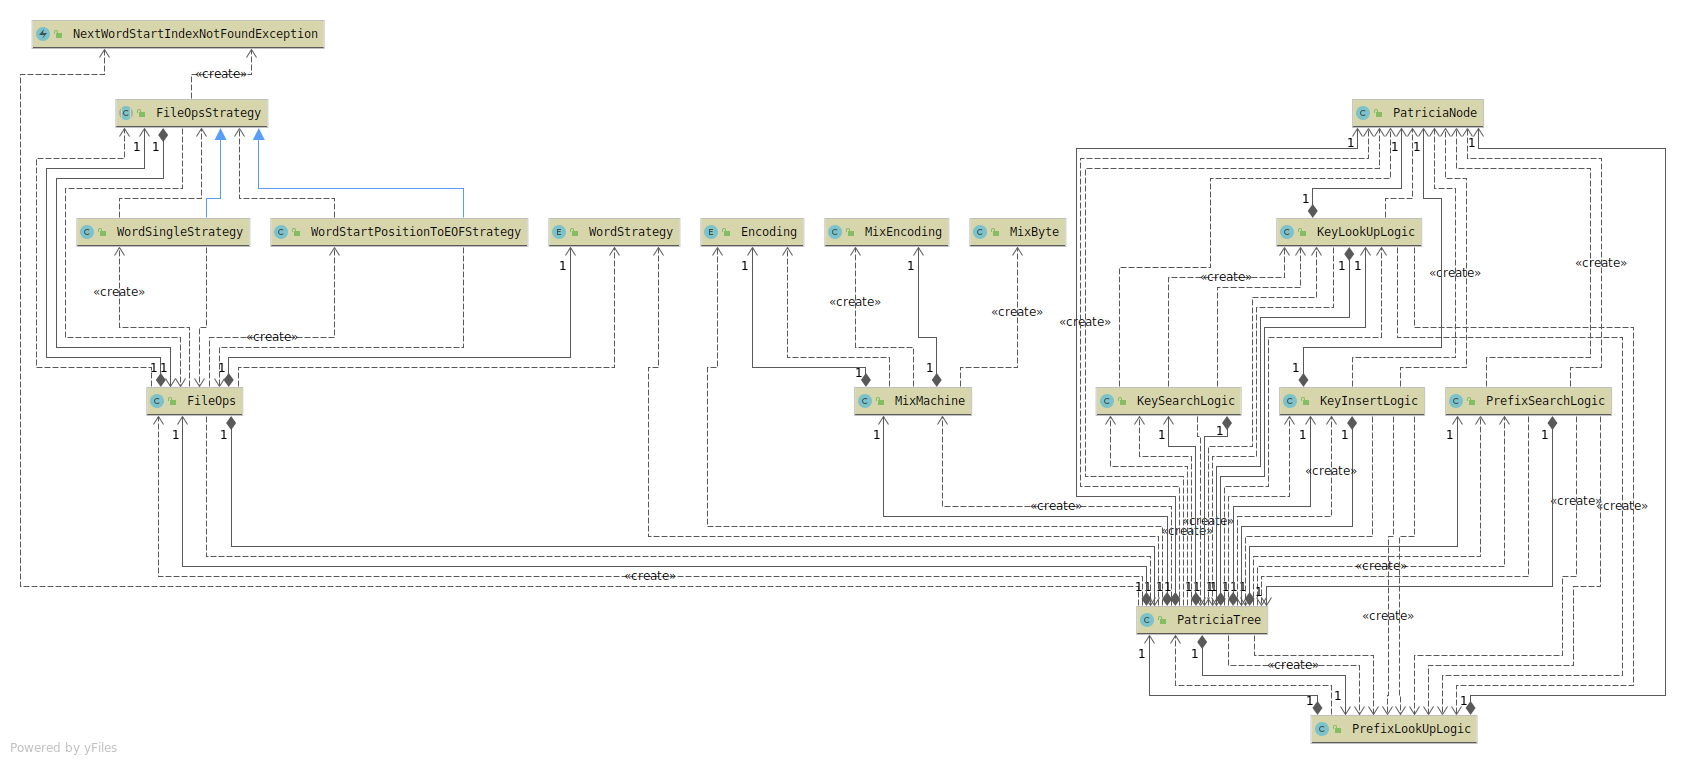
\includegraphics[angle=90,height = 0.95\textheight]{Class_Diagram_white.png}
\end{figure}
		
		% itd.
		\makeatother%
	\end{appendices}
	
\end{document}
